% Created 2016-06-01 Wed 21:34
\documentclass[11pt]{article}
\usepackage[utf8]{inputenc}
\usepackage{lmodern}
\usepackage[T1]{fontenc}
\usepackage{fixltx2e}
\usepackage{graphicx}
\usepackage{longtable}
\usepackage{float}
\usepackage{wrapfig}
\usepackage{rotating}
\usepackage[normalem]{ulem}
\usepackage{amsmath}
\usepackage{textcomp}
\usepackage{marvosym}
\usepackage{wasysym}
\usepackage{amssymb}
\usepackage{amsmath}
\usepackage[version=3]{mhchem}
\usepackage[numbers,super,sort&compress]{natbib}
\usepackage{natmove}
\usepackage{url}
\usepackage{minted}
\usepackage{underscore}
\usepackage[linktocpage,pdfstartview=FitH,colorlinks,
linkcolor=blue,anchorcolor=blue,
citecolor=blue,filecolor=blue,menucolor=blue,urlcolor=blue]{hyperref}
\usepackage{attachfile}
\usepackage{siunitx}
\usepackage[left=1in, right=1in, top=1in, bottom=1in, nohead]{geometry}
\geometry{margin=1.0in}
\usemintedstyle{emacs}
\newminted{python}{fontsize=\normalsize}
\usepackage{framed,color}
\definecolor{shadecolor}{rgb}{1.0,0.8,0.3}
\usepackage{fancyhdr}
\pagestyle{fancy}
\fancyhf{}
\renewcommand{\headrulewidth}{0.5pt}
\renewcommand{\footrulewidth}{0.5pt}
\lfoot{\today}
\cfoot{\copyright\ 2016 W.\ F.\ Schneider}
\rfoot{\thepage}
\author{William F. Schneider}
\date{\today}
\title{Lecture Notes for CBE 20255}
\begin{document}

\tableofcontents

\begin{options}
\end{options}

\section{Revised order}
\label{sec-1}
\begin{itemize}
\item variables
\item mass balances, single phase, mixtures, \ldots{}
\begin{itemize}
\item systems of linear equations
\end{itemize}
\item energy balances, single phase, mechanical, \ldots{}
\item single component, two-phase
\item two-component, two-phase, ideal
\item reactions
\item two-component, two-phase, non-ideal
\end{itemize}

\section{Intro to Chemical Engineering}
\label{sec-2}
\begin{enumerate}
\item Pop quiz
\begin{enumerate}
\item Which weighs more, the Earth or the moon?
\item Mix together 100 mL \ce{H2O} and 50 mL alcohol.  What's the final volume?
\item Add 10 g Fe ball at 100 C to 10 g H2O at 20 C.  What's the final temperature?
\item My pool holds 20,000 gal of \ce{H2O}.  Pump circulates at 10 gpm.  How
long does it take for all the \ce{H2O} to pass through the filter?
(Depends on whether it recirculates!)
\end{enumerate}
\item Instructor
\item Students
\item Syllabus
\item Assignment: Read Chapter 1
\end{enumerate}
\section{Introduction to Engineering Calculation}
\label{sec-3}
\subsection{Objectives}
\label{sec-3-1}
\begin{enumerate}
\item unit conversions
\item SI, cgs, English systems
\item sig figs
\item Is my answer reasonable?
\item Basic stats
\item Data fitting
\end{enumerate}
\subsection{Units and dimensions}
\label{sec-3-2}
\begin{itemize}
\item Engineering always deal with quantifiable, computable things.
\item Anything we can quantify has a \textbf{value} (number) and a \textbf{unit} (number of what? meters, bananas, bits, seconds)
\item A \textbf{dimension} is a property of a quantity, like \emph{length}, \emph{time}, \emph{speed} = \emph{length} / \emph{time}, \emph{density} = \emph{mass} / \emph{volume}.  Most physical quantities have a dimension (other than pesky dimensionless quantities!).
\item Quantities of the \textbf{same dimension} can be added or subtracted.  First they have to be put into the \textbf{same units}.
\end{itemize}

\[\boxed{\SI{3}{cm}+\SI{43}{mm} = \SI{30}{mm} + \SI{43}{mm} = \SI{73}{mm}} \]

\begin{itemize}
\item Quantities of different dimension can be multiplied or divided and carry the combined dimension
\end{itemize}
\[\boxed{ \SI{44}{m} / \SI{11}{s} = \SI[per-mode=symbol]{4}{\m\per\s}} \]

\begin{itemize}
\item Units \emph{not welcome} inside transcendental functions, sin, cos, ln, \ldots

\item Equations must be \emph{dimensionally homogeneous}: all additive terms on either side of an equality must have the same units

\item \textbf{ALWAYS} carry units in engineering computations
\end{itemize}

\subsection{Systems of units}
\label{sec-3-3}
\begin{itemize}
\item Base units
\end{itemize}

\begin{center}
\begin{tabular}{llll}
\hline
Dimension & SI & cgs & English\\
\hline
Length & m & cm & in, ft, mi\\
Mass & kg & g & lb$_{\text{m}}$\\
Time & s & s & s\\
Temperature & K & K & F\\
Current & A & A & \\
Light intensity & cd & cd & \\
\hline
\end{tabular}
\end{center}

\begin{itemize}
\item Multiplicative factors: T, G, M, k, c, d, m, $\mu$, n, f

\item Important chemical eng. derived units
\end{itemize}
\begin{center}
\begin{tabular}{llll}
\hline
Volume & liter & L & 1000 cm$^{\text{3}}$\\
Force & Newton & N & 1 kg m/s$^{\text{2}}$\\
 & dyne &  & 1 g cm/s$^{\text{2}}$\\
Energy/Work & Joule & J & 1 N m = 1 kg m$^{\text{2}}$/s$^{\text{2}}$\\
 & erg &  & 1 dyne cm = 1 g cm$^{\text{2}}$/s$^{\text{2}}$\\
 & calorie & cal & 4.184 J\\
 & Btu &  & 1 Btu = 1055.05585 J\\
Power & Watt & W & 1 J/s\\
 & Horsepower & hp & 1 hp = 745.7 W\\
Pressure & Pascal & Pa & 1 N/m$^{\text{2}}$ = 1 J/m$^{\text{3}}$\\
 & bar &  & 10$^{\text{5}}$ Pa\\
 & atmosphere & atm & 1 atm = 1.01325 bar\\
 & torr & torr & 1/760 atm\\
\hline
\end{tabular}
\end{center}

\begin{itemize}
\item Inside book cover has many useful conversions

\item Fun facts: 1 L of \ce{H2O} has a mass of 1 kg or about 2.2 lb$_{\text{m}}$.  What about a liter of gasoline?

\item Fun facts: 1 Btu is amount of heat released in burning 1 4 in wood match, or heat needed to raise the temperature of 1 lb$_{\text{m}}$ water by 1$^{\^{}}$ F. ``Horsepower'' used by Watt to compare the power output of a draft horse to his steam engine.  Definitions abound!
\item Pain in the neck to go between systems of units.  Need conversion factors.  E.g,. 1 lb$_{\text{m}}$ = 453.5932 g.  1 in = 2.54 cm.  Unless \emph{forced} otherwise, use SI!
\end{itemize}

\subsection{Unit conversions}
\label{sec-3-4}
\begin{itemize}
\item Conversion factors are ratios
\end{itemize}

\[ \boxed{\SI[per-mode=fraction]{4}{\m\per\s} * \SI[per-mode=fraction]{100}{\cm\per\m} = \SI[per-mode=fraction]{400}{\cm\per\s}} \]

\begin{itemize}
\item Conversion factors can be ganged.  Example: show that
\end{itemize}
\[ \boxed{\SI{1.00}{\cm\per\s\squared} = \SI{9.95e9}{\km\per year\squared}} \]

\subsection{Dimensional homogeneity}
\label{sec-3-5}
\begin{framed}
\noindent As you will learn in Thermodynamics, the internal energy \(U\) is related to other thermodynamic quantities by  the relation
\begin{equation}
U = T S - P V + \mu N
\end{equation}
\noindent What are units on the entropy, \(S\)?  Chemical potential, \(\mu\)?  What does this say about the dimensionality of pressure?
\end{framed}


\begin{framed}
\noindent The Schr\"{o}dinger equation is the fundamental equation of quantum mechanics:
\begin{equation}
-\frac{\hbar^{2}}{2 m} \frac{\partial^{2}\psi}{\partial x^{2}} + V(x) \psi = E \psi
\end{equation}
\(E\) has units of energy and \(m\) units of mass.  What are the units on \(V(x)\)?  \(\hbar\)?  \(\psi(x)\)?
\end{framed}

\subsection{Mass, force, weight}
\label{sec-3-6}
\begin{itemize}
\item \emph{mass} of an object is an intrinsic property, resistance to an applied force
\item Newton's 3rd Law
\end{itemize}
\[\boxed{F = m a } \]
\begin{itemize}
\item English force units messy
\end{itemize}
\[\boxed{\SI{1}{lb_{f}}=\SI{32.174}{lb_{m} ft\per\s\squared}} \]
\begin{itemize}
\item \emph{weight} is force exerted by a gravitational field on a mass
\end{itemize}
\[ \boxed{w = m g} \]
\begin{itemize}
\item \emph{g} depends on the planet you are standing on, as well as where you are standing
\end{itemize}
\begin{eqnarray*}
g &= & \SI{9.8066}{\m\per\s\squared}\\
  & = & \SI{32.174}{ft\per\s\squared}
\end{eqnarray*}

\begin{framed}
\noindent Water has a density of \( \SI{62.4}{lb_{m}\per ft\cubed}\).  How much does 2 ft$^{3}$ of water weigh on the earth?  On the moon (\(g = \SI{1.62519}{\m\per\s\squared})?
\end{framed}
\begin{minted}[frame=lines,fontsize=\scriptsize,linenos]{python}
earth = 2 * 62.4 * 32.174 * (1./32.174)
moon = earth * 1.62519/9.8066
print('earth:',earth,'lbf')
print('moon:',moon,'lbf')
\end{minted}

\begin{verbatim}
earth: 124.80000000000001 lbf
moon: 20.682368201007485 lbf
\end{verbatim}

\subsection{Numerical calculations}
\label{sec-3-7}
\subsubsection{Scientific notation, significant figures, precision}
\label{sec-3-7-1}
\begin{itemize}
\item Significant figures imply a precision
\item \emph{Always} report numbers with reasonable significant figures.
\item Examples of adding and multiplying with sig figs.
\item Round to even number: 1.35 to 1.45 all round to 1.4.
\end{itemize}
\subsubsection{Validating results}
\label{sec-3-7-2}
\begin{itemize}
\item Does the result make physical sense?
\item Do a ballpark estimate.
\item Back-substitute
\end{itemize}
\subsubsection{Sources of error}
\label{sec-3-7-3}
\begin{itemize}
\item Few, if anything, can be measured exactly.  Processes have intrinsic variability
\item CSTR example: flow rate may fluctuate, temperature fluctuate, slightly inhomogeneous.  So do measurements (thermocouple).  Best we can do is estimate the ``truth.''
\begin{itemize}
\item random error
\item systematic error
\item Show random scatter, systematic drift, oscillation
\end{itemize}
\end{itemize}

\begin{minted}[frame=lines,fontsize=\scriptsize,linenos]{python}
import numpy as np
import matplotlib.pyplot as plt
x = np.arange(40.)
sigma = 1.
T = 25. + sigma*np.random.randn(40)
T1 = 20. + .2 * x + sigma*np.random.randn(40)
T2 = 25. + 4. * np.sin(x/4.) + sigma*np.random.randn(40)

plt.subplot(311)
plt.scatter(x,T)
plt.ylim(15,35)
plt.xlim(0,40)
plt.ylabel('Temperature (C)')

plt.subplot(312)
plt.scatter(x,T1)
plt.ylim(15,35)
plt.xlim(0,40)
plt.ylabel('Temperature (C)')

plt.subplot(313)
plt.scatter(x,T2)
plt.ylim(15,35)
plt.xlim(0,40)
plt.xlabel('Sample (hour)')
plt.ylabel('Temperature (C)')
plt.savefig('./figs/random.png')
\end{minted}

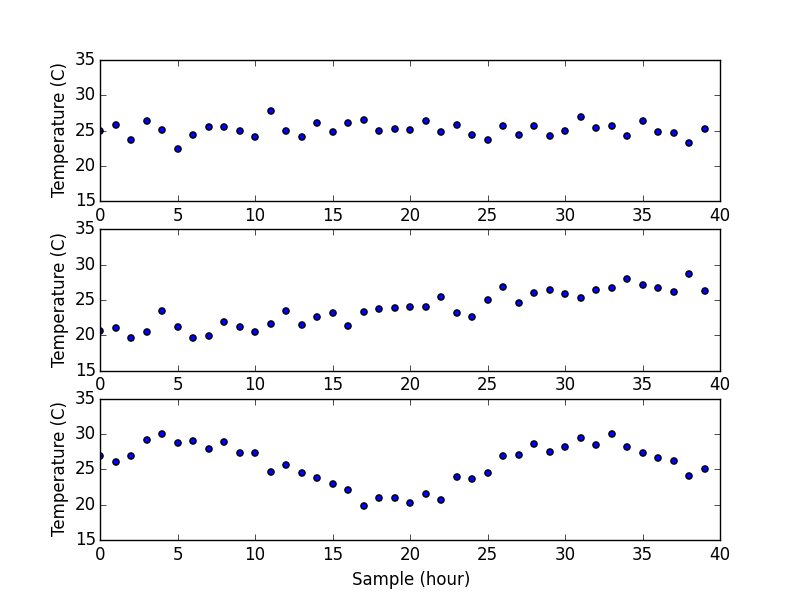
\includegraphics[width=.9\linewidth]{./figs/random.png}

\subsubsection{Sample mean}
\label{sec-3-7-4}
\begin{itemize}
\item \emph{sample mean} to estimate truth
\end{itemize}
\[\boxed{\bar{X}=\sum_{1}^{n}X_{i}} \]

\subsubsection{Measures of scatter}
\label{sec-3-7-5}
\begin{itemize}
\item \emph{Range}
\item \emph{Sample variance}
\end{itemize}
\[\boxed{s_{X}^{2}=\frac{1}{N-1}\sum_{1}^{n}(X_{i}-\bar{X})^{2}}\]
\begin{itemize}
\item \emph{Standard deviation} has same units as \emph{X}
\end{itemize}
\[\boxed{s_{x}=\sqrt{s_{X}^{2}}} \]
\begin{itemize}
\item If a random variable is Gaussian, about 2/3 of measurements are within \(s_{x}\) of the mean, 95\% within \(2s_{x}\), 99\% within \(3s_{x}\).
\item Example 2.5.2
\end{itemize}

\begin{framed}
\noindent QA on pigment.  Let \(Y\) be the number of batches that fail QA out of 500 in a week.  If process is shutdown for maintenance if \(Y > \bar{Y} + 3 S_{Y}\), how many bad batches are required for a shutdown?
\end{framed}

\begin{minted}[frame=lines,fontsize=\scriptsize,linenos]{python}
import numpy as np
import matplotlib.pyplot as plt

Week = np.array([1, 2, 3, 4, 5, 6, 7, 8, 9, 10, 11, 12])
Y = np.array([17,  27,  18,  18,  23,  19,  18,  21,  20,  19,  21,  18 ])
plt.scatter(Week,Y)
plt.ylim(0,30)
plt.xlabel('Week')
plt.ylabel('Fails out of 500')
plt.savefig('./figs/QA.png')

N = Y.size
Sum = np.sum(Y)
Average = Sum/N

Variance = np.sum((Y - Average)**2)/(N-1)
StdDev = Variance**0.5

print('N   Sum   Average  Variance  Std. Dev')
print("{0:3d} {1:4d} {2:5.2f}   {3:5.2f}   {4:5.2f}".format(N,Sum,Average,Variance,StdDev))

Shutdown = Average + 3 * StdDev
print('Shutdown if Y > {0:5.2f}'.format(Shutdown))
\end{minted}

\begin{verbatim}
N   Sum   Average  Variance  Std. Dev
 12  239 19.92    7.90    2.81
Shutdown if Y > 28.35
\end{verbatim}

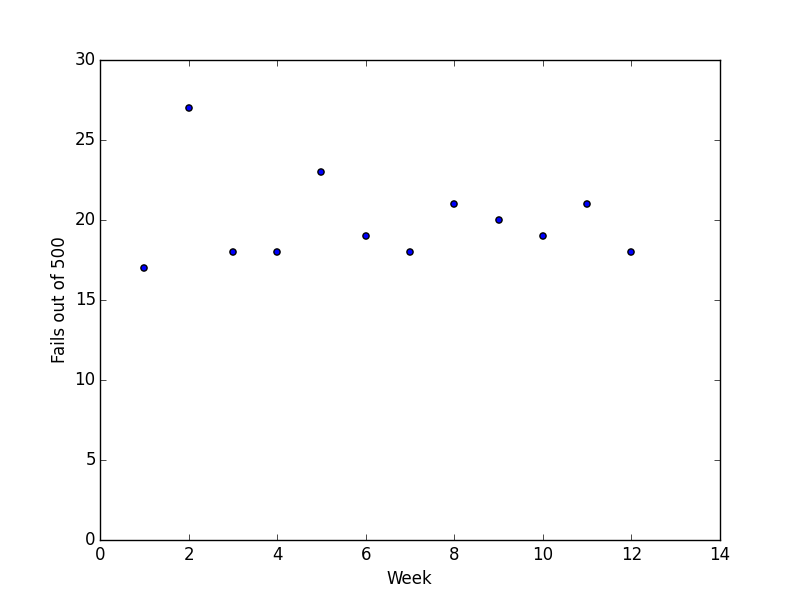
\includegraphics[width=0.5\textwidth]{./figs/QA.png}

\subsection{Process data modeling}
\label{sec-3-8}
\begin{itemize}
\item Often interested in the relationship between two correlated variables.  E.g. a correlation curve between a thermocouple resistance and a temperature.  An optical density and a concentration.
\item \emph{Linear regression} to fit linear data (Appendix A); minimizes \emph{residuals} between data and a fit line
\item \(r^{2}\) measures fraction of variance in \emph{y} ``explained'' by variance in \emph{x}; 1 is best, 0 is worst
\end{itemize}
\[ r^{2} = 1. - \frac{\sum \text{res}_\text{lg}^{2}}{\sum \text{res}_\text{null}^{2}} \]
\begin{itemize}
\item Linearizing data (e.g. Arrhenius plot).  (\emph{Danger}: Error can be scewed by linearizing.  Non-linear regression a good alternative.)
\end{itemize}

\begin{minted}[frame=lines,fontsize=\scriptsize,linenos]{python}
import numpy as np
import matplotlib.pyplot as plt
from scipy import stats

EHxy = [ 144,144, 132, 132, 116, 116, 190, 190, 173, 173, 111, 111, 91, 91, 207, 207, 199, 199, 110, 110, 83, 83]
RDxy = [152, 150, 141, 134, 117, 117, 204, 202, 184, 183, 123, 118, 94, 96, 225, 224, 213, 213, 114, 115, 89, 93]

m, b, r, p, e = stats.linregress(EHxy,RDxy)
print("Slope       Intercept          r**2")
print(m,b,r**2)

nu = np.linspace(80,230)
fit = m * nu + b

plt.scatter(EHxy,RDxy)
plt.plot(nu,fit)
plt.xlim((50,250))
plt.ylim((50,250))
plt.xlabel('Effective harmonic frequencies (cm$^{{-1}}$)')
plt.ylabel('Relaxed displacement frequencies (cm$^{{-1}}$)')
plt.savefig('./figs/freq.png')
\end{minted}

\begin{verbatim}
Slope       Intercept          r**2
1.08962211596 -4.08654658558 0.995318037198
\end{verbatim}

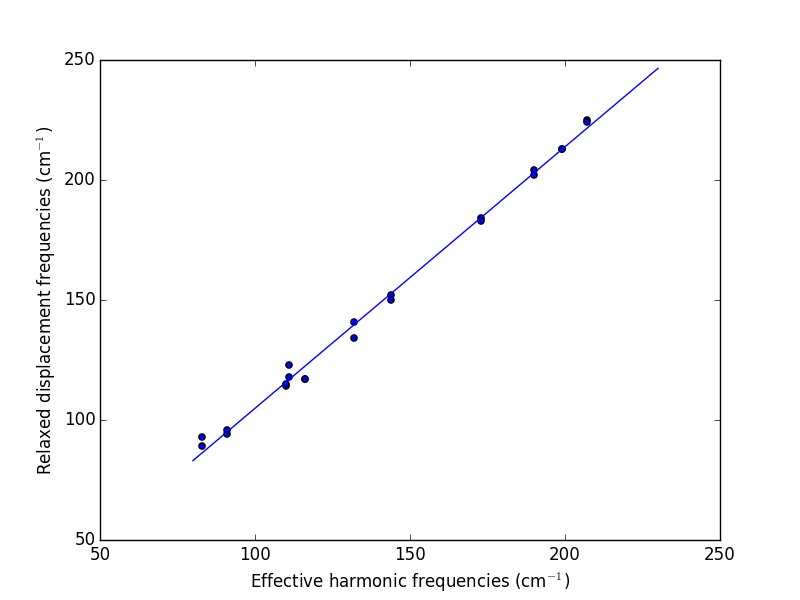
\includegraphics[width=0.5\textwidth]{./figs/freq.png}

\newpage

\section{Processes and process variables}
\label{sec-4}
\subsection{Learning objectives}
\label{sec-4-1}
\begin{itemize}
\item density
\item flow rates
\item composition
\item pressure
\end{itemize}
\subsection{Mass, volume, density}
\label{sec-4-2}
\begin{itemize}
\item mass, volume are \emph{extensive} quantities
\item \emph{density} ($\rho$) = mass / volume is \emph{intensive}, characteristic of a substance at some \emph{T} and \emph{P}
\item tabulated in common handbooks, allows us to convert between \emph{m} and \emph{V}
\item \emph{specific gravity} is density relative to some reference, commonly \ce{H2O} at \SI{4}{\celsius}
\end{itemize}
\begin{equation}
 \rho_{\ce{H2O}}(\SI{4}{\celsius}) = \SI{1.00}{\gram\per\cm\cubed} = \SI{62.43}{lb_{m}\per ft\cubed}
\end{equation}
\begin{itemize}
\item mass is independent of \emph{T}, volume changes with \emph{T}, therefore so does $\rho$
\item can find tabulations of \(\rho(T)\), \(V(T)\), or \emph{coefficient of thermal expansion}
\end{itemize}
\begin{equation}
\alpha(T) = \frac{1}{V}\left ( \frac{\partial V}{\partial T} \right )_{P}
\end{equation}
\begin{itemize}
\item \textbf{Example 3.1.1}
\end{itemize}

\begin{quote}
Specific gravity of Hg at \SI{20}{\celsius} is 13.456.  Density?  Volume of 215 kg?
\end{quote}

\begin{minted}[frame=lines,fontsize=\scriptsize,linenos]{python}
rho = 13.546 * 62.43
print('Density = ',rho,' lbm/ft^3')
print('Volume = mass/density')
volume = 215 * (1./0.454) / rho
print('Volume =',volume,'ft3')
\end{minted}

\begin{verbatim}
Density =  845.67678  lbm/ft^3
Volume = mass/density
Volume = 0.5599873298381516 ft3
\end{verbatim}

\hline
\begin{itemize}
\item \textbf{Example 3.1.2}
\end{itemize}

\begin{quote}
(a) What is volume of 215 kg Hg at \SI{100}{\celsius}?

(b) What is change in height between 20 and \SI{100}{\celsius} of a 0.25 in diameter Hg cylinder?
\end{quote}
\[ V_{Hg}(T) = V(0) [ 1 + 0.18182\times 10^{-3} T + 0.0078\times 10^{-6} T^{2} ] \]
\[ V(100) = V(20) * \frac{V(100)}{V(20)} \]
\[h = V/A\]

\begin{minted}[frame=lines,fontsize=\scriptsize,linenos]{python}
import numpy as np

def V(T):
# Volume relative to volume at 0 C
    a = 0.18182e-3
    b = 0.0078e-6
    return 1. + T * (a + b*T)
def h(V):
    area = np.pi * (0.25/12./2.)**2
    return V/area

V20 = 0.560
h20 = h(V20)
V100 = V20 * V(100.)/V(20.)
h100 = h(V100)
print('Temperature    Volume (ft3)   Height (ft)')
print("{0:8.1f}       {1:6.3f}       {2:6.2f}".format(20,V20,h20))
print("{0:8.1f}       {1:6.3f}       {2:6.2f}".format(100,V100,h100))

deltah = h100-h20
print("Delta h = {0:6.2f} ft".format(deltah))
\end{minted}

\begin{verbatim}
Temperature    Volume (ft3)   Height (ft)
    20.0        0.560       1642.78
   100.0        0.568       1666.72
Delta h =  23.93 ft
\end{verbatim}

\hline
\subsection{Flow rate}
\label{sec-4-3}
\begin{itemize}
\item mass flow rate \(\dot{m}\): mass passing an area in a time
\item volume flow rate \(\dot{V}\): volume passing an area in a time
\end{itemize}

\[\rho =\frac{m}{V}=\frac{\dot{m}}{\dot{V}} \]

\begin{itemize}
\item Gas flows down a tapered cone.  How does mass flow rate compare at entrance and exit?
\begin{itemize}
\item Same
\end{itemize}
\item If density is constant, how does volumetric flow rate compare?
\begin{itemize}
\item Same
\end{itemize}
\item How does linear velocity compare
\begin{itemize}
\item Goes up!
\end{itemize}
\item Molar flow rate, \(\dot{F}\)?  Need to know MW!
\end{itemize}

\subsection{Chemical composition}
\label{sec-4-4}
\subsubsection{Moles and molecular weights}
\label{sec-4-4-1}
\begin{itemize}
\item atomic theory, we can count atoms and molecules.  They are tiny, so need a big unit to count with!
\item molecular ``weight'' (\emph{MW}) is mass relative to \ce\{$^{\text{12}}$C\}, defined to have a mass of 12
\item Avogadro's number \(N_{A}=6.022\times 10^{23}\) number of \ce\{$^{\text{12}}$C\} to make 12 grams, called a \texttt{mole} or \texttt{gram-mole} (yech!)
\item \texttt{kmol} makes 12 kg, \texttt{lb-mole} makes 12 lbm
\item periodic table records masses of all elements relative to \ce{12C}
\end{itemize}

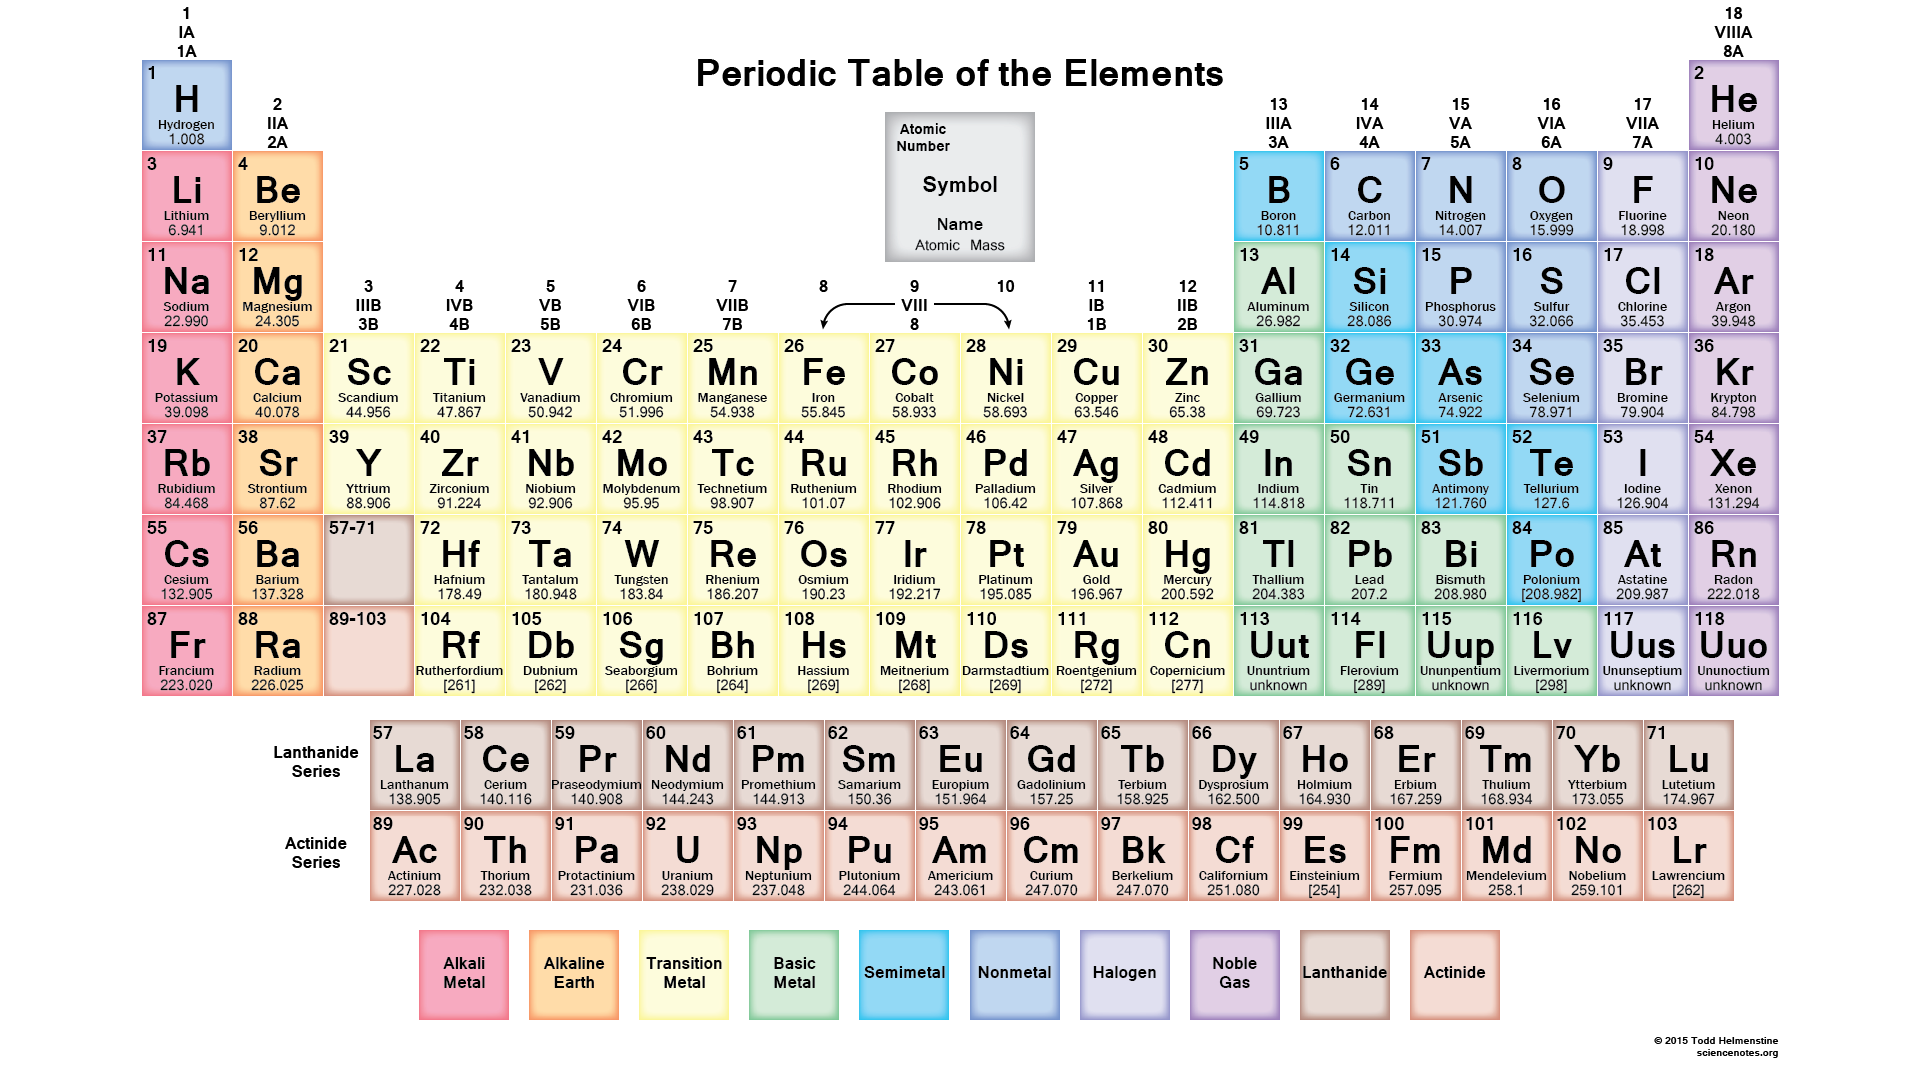
\includegraphics[width=.9\linewidth]{./figs/PeriodicTableMuted.png}

\begin{itemize}
\item \ce{CO2} = 44 g/g-mol = 44 kg/kg-mol = 44 lbm/lb-mol = 44 ton/ton-mol
\item calculate molar flow rate from mass flow rate
\end{itemize}
\begin{quote}
\textbf{EXAMPLE} What is molar flow rate of O in a stream of 4400 kg/hr \ce{CO2}?
\end{quote}

\begin{minted}[frame=lines,fontsize=\scriptsize,linenos]{python}
F = 4400 * (1./44.) * 2
print("{0:6.2f} kmol O/hr".format(F))
\end{minted}

\begin{verbatim}
200.00 kmol/hr
\end{verbatim}

\subsection{Mixtures}
\label{sec-4-5}
\begin{itemize}
\item Always expressed as something/something
\item Generally faced with two types of problems: turn one concentration measure into another (intensive $\to$ intensive); or use in conversions of extensive $\to$ extensive
\end{itemize}
\subsubsection{Mass and mole fractions}
\label{sec-4-5-1}
\begin{itemize}
\item mass fraction A = mass A/total mass
\item mole fraction A = mol A/total mol
\item vol fraction A = vol A/total vol
\end{itemize}

\begin{quote}
\textbf{EXAMPLE} 35.0 \%(w/w) \ce{H2SO4} has a specific gravity of 1.2563.  What volume of solution is needed to obtain 500 g-mol \ce{H2SO4}? (Extensive to extensive)
\end{quote}
\begin{minted}[frame=lines,fontsize=\scriptsize,linenos]{python}
MW = 2.*(1.008) + 32.0 + 4 * 16.0   # g/g-mol
mass = 500 * MW                     # g
mass_soln = mass * (100./35.0)      # g
rho = 1.2563                        # g/mL
volume = mass_soln/rho/1000         # L
print("Volume={0:6.3f} L".format(volume))
\end{minted}

\begin{verbatim}
Volume=111.457 L
\end{verbatim}


\begin{quote}
\textbf{EXAMPLE} What is mole fraction \ce{H2SO4} in 35.0\%(w/w) solution? (intensive to intensive)
\end{quote}
\begin{minted}[frame=lines,fontsize=\scriptsize,linenos]{python}
MWH2SO4 = 2*1.008 + 32.0 + 4 * 16.00
MWH2O = 2 *1.008 + 16.00

molH2SO4 = 35.0 / MWH2SO4    # mol H2SO4
molH2O   = (100.-35.0)/ MWH2O # mol H2O

fracH2SO4 = molH2SO4/(molH2SO4+molH2O)

print("{0:6.3f}%(mol/mol) H2SO4".format(fracH2SO4*100))
\end{minted}

\begin{verbatim}
9.006%(mol/mol) H2SO4
\end{verbatim}

\begin{itemize}
\item trace species in a gas often expressed as ppm or ppb rather than \%
\item EPA ozone standard is 70 ppb, 70 ozone molecules/billion molecules of air
\item less frequently mass rather than mole basis
\end{itemize}
\subsubsection{Average molecular weight}
\label{sec-4-5-2}
\[ \bar{MW} = \sum_{i} y_{i} MW_{i} \]

\begin{quote}
\textbf{EXAMPLE} What is average molecular weight of air, which is 76.7\% \ce{N2} and 23.3\% \ce{O2} by mass?
\end{quote}

\begin{minted}[frame=lines,fontsize=\scriptsize,linenos]{python}
# 100 g basis
MWN2 = 28.0
MWO2 = 32.0
molN2 = 76.7 / MWN2
molO2 = 23.3 / MWO2
moltot= molN2 + molO2
fracN2 = molN2/moltot
fracO2 = molO2/moltot
MWbar = fracN2*MWN2 + fracO2*MWO2

print("100 g basis")
print("              N2      O2")
print("MW:          {0:4.2f}    {1:4.2f}".format(MWN2,MWO2))
print("moles:       {0:4.2f}    {1:4.2f}".format(molN2,molO2))
print("mole frac:   {0:4.2f}    {1:4.2f}".format(fracN2,fracO2))
print("\nMWbar = {0:6.2f} g/mol".format(MWbar))
\end{minted}

\begin{verbatim}
100 g basis
              N2      O2
MW:          28.00    32.00
moles:       2.74    0.73
mole frac:   0.79    0.21

MWbar =  28.84 g/mol
\end{verbatim}

\subsubsection{Concentrations}
\label{sec-4-5-3}
\begin{itemize}
\item ``concentration'' sometimes reserved for amount/volume
\item \texttt{molarity} = mol/volume; mass/volume less common
\end{itemize}

\begin{quote}
\textbf{EXAMPLE} 0.50 M \ce{H2SO4} flows into a process unit at \SI{1.25}{\meter\cubed\per\minute}.  S.G. = 1.03.  (a) Mass concentration? (b) mass flow rate of \ce{H2SO4}? (c) mass fraction \ce{H2SO4}?
\end{quote}

\begin{minted}[frame=lines,fontsize=\scriptsize,linenos]{python}
Molarity = 0.50                # mol/L
MW  = 2*1.0 + 32.0 + 4 * 16.0  # g/mol
flow = 1.25                    # m3/min
density = 1.03                 # kg/L

mass_conc = Molarity * (MW) * (1/1000) * (1000/1)  # kg H2SO4/m3

H2SO4_mass_flow = mass_conc * flow * (1/60)          # kg H2SO4/s

total_mass_flow = flow * (1/60) * (1000/1) * density  # kg/s

mass_frac = H2SO4_mass_flow/total_mass_flow

print("{0:5.2f} kg H2SO3/m3   {1:5.2f} kg/s   {2:5.4f} kg H2SO4/kg".format(mass_conc,H2SO4_mass_flow,mass_frac))
\end{minted}
\begin{verbatim}
49.00 kg H2SO3/m3    1.02 kg/s   0.0476 kg H2SO4/kg
\end{verbatim}

\subsection{Pressure}
\label{sec-4-6}
\subsubsection{Measures of pressure}
\label{sec-4-6-1}
\begin{itemize}
\item Pressure = Force/area required to resist motion of a frictional piston against a fluid
\item Internal fluid pressure arises from molecular motions and is present in any confined fluid
\item \emph{hydrostatic pressure} arises from gravitational force
\end{itemize}

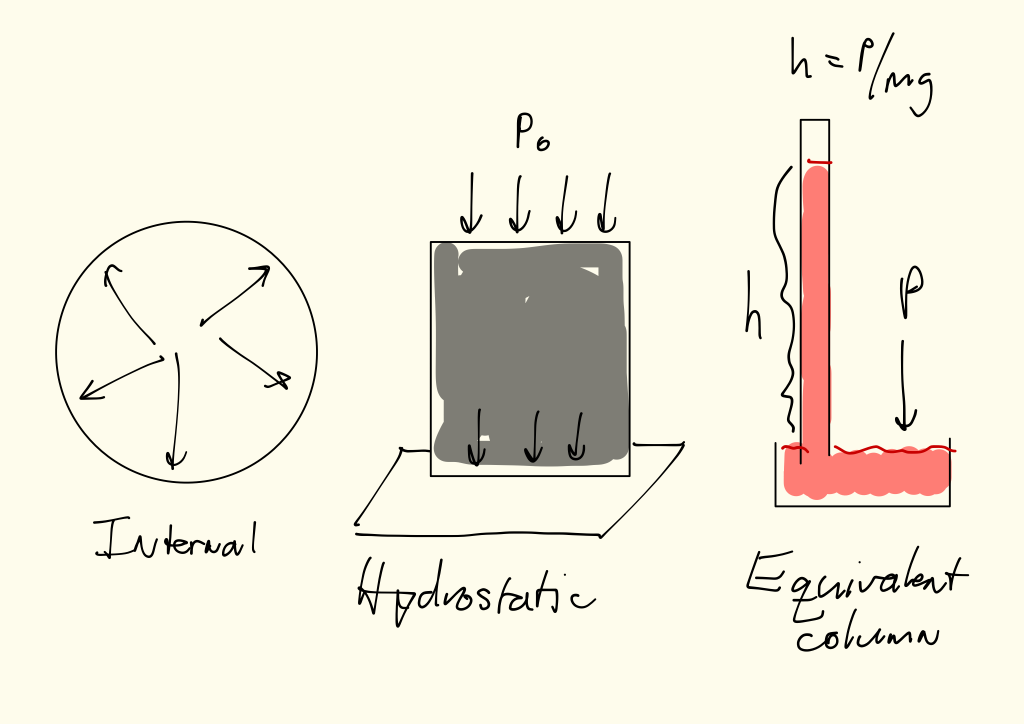
\includegraphics[width=0.8\textwidth]{./figs/Pressure.png}

\begin{itemize}
\item \emph{air pressure} is hydrostatic pressure of the atmosphere (1 atm)
\item measured in standard pressure units (Pa, bar, atm)
\item \emph{or} measured in equivalent height of a fluid column in vacuum, most commonly mmHg, \(\rho_{\ce{Hg}} = \SI{13.6}{\gram\per\cm\cubed} = \SI{13594}{\kilogram\per\meter\cubed} (\SI{0}{\celsius}) \)
\end{itemize}

\begin{framed}
\[ h = P / \rho  g \]
\end{framed}

\begin{quote}
\textbf{EXAMPLE} Express 1 atm in mmHg and mmH2O.
\end{quote}

\begin{minted}[frame=lines,fontsize=\scriptsize,linenos]{python}
pressure = 1.01325e5 # Pa
density = 13594.  # kg/m3
g = 9.807  #  m/s2

heightHg = pressure /(density * g) # m
heightH2O = 13.6 * heightHg
print('{0:6.1f} mmHg   {1:8.2f} mH2O'.format(heightHg*1000,heightH2O))
\end{minted}

\begin{verbatim}
760.0 mmHg      10.34 mH2O
\end{verbatim}

\begin{itemize}
\item open column of fluid (or solid) will have a total hydrostatic pressure at the base of atmospheric pressure plus column pressure
\end{itemize}
\[ P = P_{0} + \rho g h \]

\begin{quote}
\textbf{EXAMPLE} Hydrostatic pressure 30.0 m below the surface of a lake?
\end{quote}

\begin{minted}[frame=lines,fontsize=\scriptsize,linenos]{python}
print('Easy way...40.3 m H2O!')

rho = 1000.   # kg/m3
g = 9.807   # m/s2
h = 30.0    # m
P0 = 1.01325e5 # Pa

pressure = P0 + rho*g*h  # Pa
pressureatm = pressure *( 1/P0)
pressurepsi = pressureatm * 14.696
print('Hard way...')
print('{0:5.2f} bar   {1:5.2f} atm    {2:5.2f} psi'.format(pressure/1e5,pressureatm,pressurepsi))
\end{minted}

\begin{verbatim}
Easy way...40.3 m H2O!
Hard way...
 3.96 bar    3.90 atm    57.37 psi
\end{verbatim}

\subsubsection{Absolute vs.~gauge}
\label{sec-4-6-2}
\begin{itemize}
\item absolute pressure = pressure relative to a vacuum, always > 0
\item gauge pressure difference from atmosphere, can be positive or negative
\[ P_{gauge} = P_{abs} - P_{atm} \]
\end{itemize}
\subsubsection{Pressure gauges}
\label{sec-4-6-3}
\begin{itemize}
\item electronic devices (e.g. piezoelectric)
\item mechanical, based on a diaphragm or other deformable object
\item manometers: two-armed device.  Pressures at equivalent heights within fluid must be the same.
\end{itemize}
\subsubsection{open-end manometer:}
\label{sec-4-6-4}
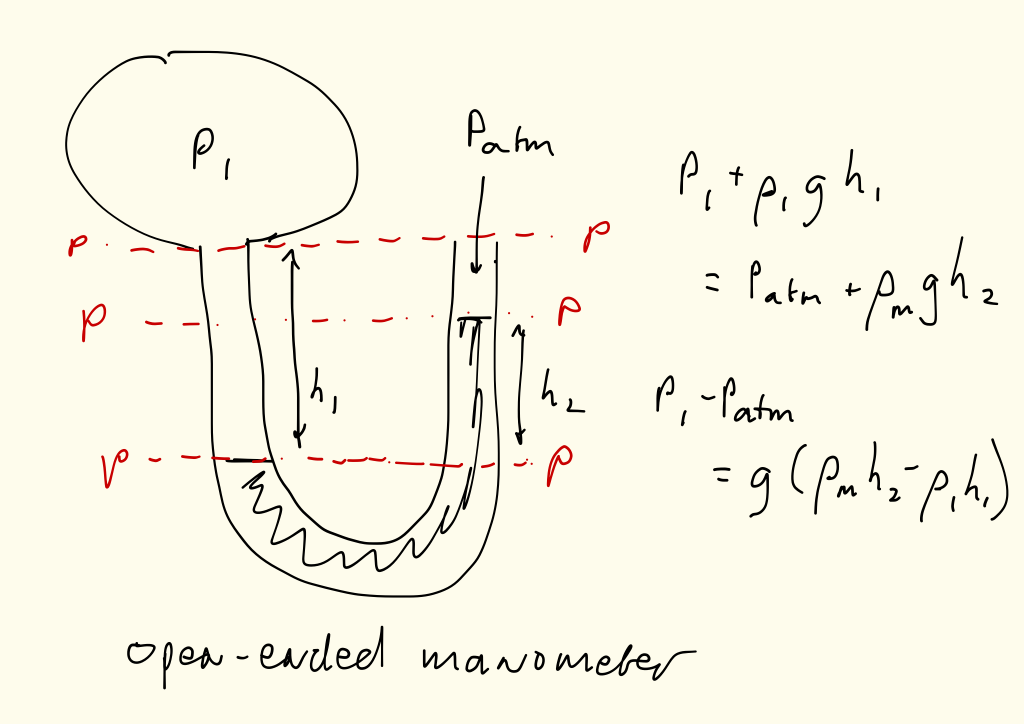
\includegraphics[width=.9\linewidth]{./figs/Manometer-open.png}
\begin{quote}
\textbf{EXAMPLE} Manometer fluid is Hg and \(h_{2} = -\SI{25}{\mm}\).  What is gauge pressure?  What is absolute pressure? In mmHg and in psi.
\end{quote}
\begin{minted}[frame=lines,fontsize=\scriptsize,linenos]{python}
hatm = 760
hgauge = -25   # mmHg
habsolute = hgauge + hatm
print('Gauge = {0:5.1f}  Abs = {1:5.1f} mmHg'.format(hgauge,habsolute))

g = 9.807      # m/s2
rhoHg = 13600  # kg/m3
pgauge = rhoHg * g * hgauge/1000.   # Pa
pabsolute = rhoHg * g * habsolute/1000.   # Pa
print('Gauge = {0:5.0f}  Abs = {1:5.0f} Pa'.format(pgauge,pabsolute))

pgauge = pgauge * (14.696/ 1.01325e5)  # lbf/in2
pabsolute = pabsolute * (14.696/ 1.01325e5)  # lbf/in2
print('Gauge = {0:5.3}  Abs = {1:5.3f} psi'.format(pgauge,pabsolute))
\end{minted}

\begin{verbatim}
Gauge = -25.0  Abs = 735.0 mmHg
Gauge = -3334  Abs = 98031 Pa
Gauge = -0.484  Abs = 14.218 psi
\end{verbatim}

\subsubsection{differential manometer}
\label{sec-4-6-5}
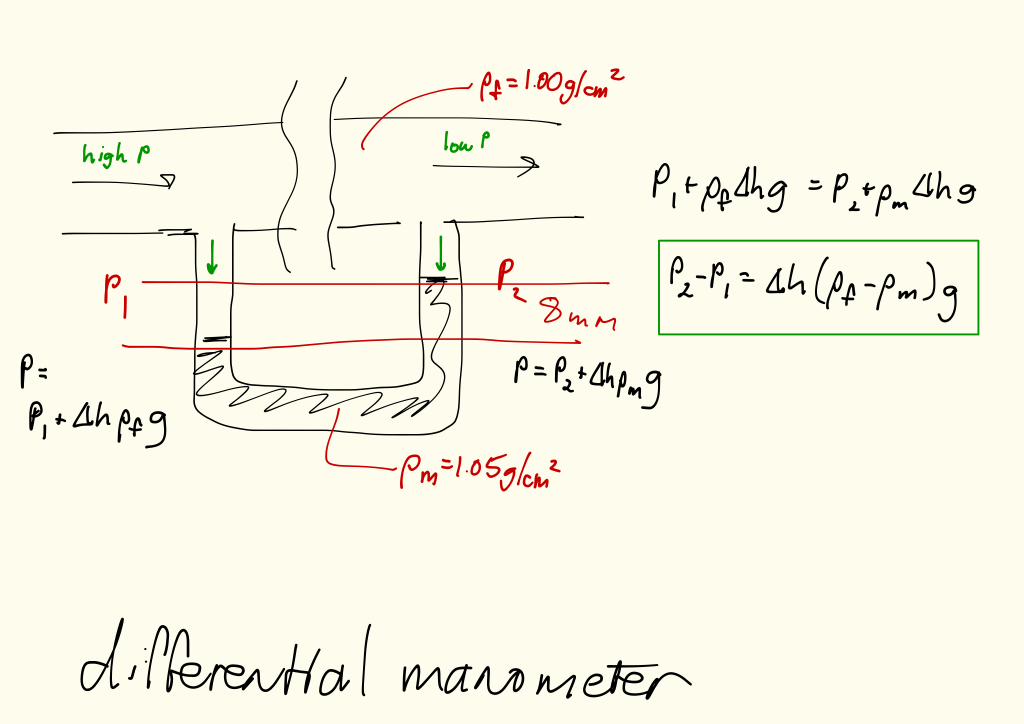
\includegraphics[width=.9\linewidth]{./figs/Manometer-diff.png}

\[ P_{2}- P_{1} = g(\rho_{f} - \rho_{m}) \Delta h \]

\begin{minted}[frame=lines,fontsize=\scriptsize,linenos]{python}
g =  980.7  # cm/s^2
Dh = 0.8    # cm
rhom = 1.05 # g/cm^3
rhof = 1.00 # g/cm^3

dP = g * Dh * (rhof - rhom) # dyne/cm2

print("\Delta P = {0:5.1f} dyne/cm2".format(dP))
\end{minted}

\begin{verbatim}
\Delta P = -39.2 dyne/cm2
\end{verbatim}

\subsubsection{Closed manometer}
\label{sec-4-6-6}
\subsection{Temperature}
\label{sec-4-7}
\subsubsection{Scales}
\label{sec-4-7-1}
\begin{itemize}
\item Kelvin: absolute scale, 0 $\to$ $\infty$
\item Celsius: \(T(^{\circ}C) = T(K) - 273.15)\)
\item Fahrenheit: \(T(^{\circ}F) = 1.8 T(^{\circ}C) + 32 )\)
\item Rankine: absolute scale, \(T(^{\circ}R) = T(^{\circ}F)+459.67\)
\item \textbf{Use care} in using in unit conversion calculations.  Ratios work for converting temperature \emph{differences}, but not for converting absolute temperatures
\end{itemize}

\subsubsection{Measurement devices}
\label{sec-4-7-2}
\begin{itemize}
\item volume-based (thermometer)
\item radiation-based (pyrometer)
\item voltage-based (thermocouple) - change in potential between two dissimilar metals
\item resistance-based (thermistor)
\end{itemize}


\newpage
\section{Material balances on non-reactive systems}
\label{sec-5}
\subsection{Process types}
\label{sec-5-1}
\begin{itemize}
\item batch
\item continuous
\item semi-batch (filling a balloon)
\item steady-state vs. transient
\end{itemize}

\subsection{General balance equation}
\label{sec-5-2}
\begin{framed}
output = input + generation - consumption - accumulation
\end{framed}

\begin{quote}
\textbf{EXAMPLE} Every year 50,000 Leute move into a city, 75,000 move out, 22,000 are born, and 19,000 die.  Write a differential balance on the population, i.e., what is change in population with time?
\end{quote}
\begin{minted}[frame=lines,fontsize=\scriptsize,linenos]{python}
input = 50000; output=75000; generation=22000; consumption=19000;
accumulation =input + generation - output - consumption
print('accumulation = {0} people/year'.format(accumulation))
\end{minted}

\begin{verbatim}
accumulation = -22000 people/year
\end{verbatim}

\begin{itemize}
\item example of \emph{differential} balance, a change over time (or space)
\item \emph{integral} balance is sum of differential balance over some unit of time or space

\item batch: input = output = 0
\item continuous, steady-state, non-reactive: accumulation = generation = consumption = 0

\item Can balance \emph{total mass}: generation = consumption = 0
\item Can balance \emph{mass} or \emph{moles} of an element or molecular species
\end{itemize}

\begin{quote}
\textbf{EXAMPLE} Differential balance on a continuous, steady-state process

\SI{1000}{\kilogram\per\hour} mixture of 50\%(w/w) benzene and toluene is distilled into two streams, one containing \SI{450}{\kilogram\per\hour} benzene and other containing \SI{475}{\kilogram\per\hour} toluene.  Solve for unknown flow rates.
\end{quote}

\includegraphics[width=.9\linewidth]{./figs/diff-balance1.png}

\subsection{Mass balance procedure}
\label{sec-5-3}
\begin{itemize}
\item Illustrates general procedure:
\end{itemize}

\hline
\begin{enumerate}
\item Create a flow chart
\item Label all known quantities along each stream
\begin{enumerate}
\item molar or mass flow rates
\item concentrations
\end{enumerate}
\item Label all \emph{unknown} quantities with symbols
\item Work in only mass or molar quantities
\end{enumerate}
\hline

\begin{itemize}
\item A flow sheet is \emph{balanced} if all material balances are closed
\item A balanced flow sheet can be \emph{scaled}; all flows multiplied by a constant value
\item Allows one to choose arbitrarily a \emph{basis}
\end{itemize}

\begin{quote}
\textbf{EXAMPLE} Air humidification example.  Three inputs are fed into an evaporation chamber:

\begin{itemize}
\item Liquid \ce{H2O}, \SI{20}{\centimeter\cubed\per\minute}
\item Air
\item \ce{O2}, at a rate 1/5 of the air
\end{itemize}

The output contains 1.5\% \ce{H20}.  What are the output compositions and other flow rates?
\end{quote}

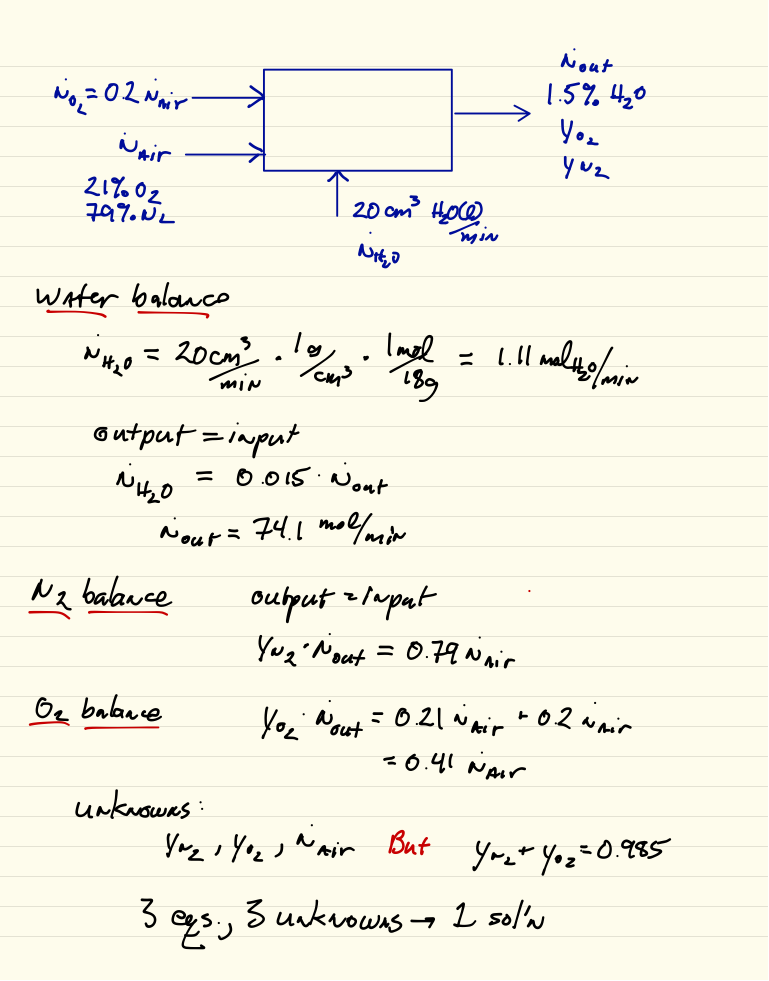
\includegraphics[width=.9\linewidth]{./figs/Diff-balance3.png}

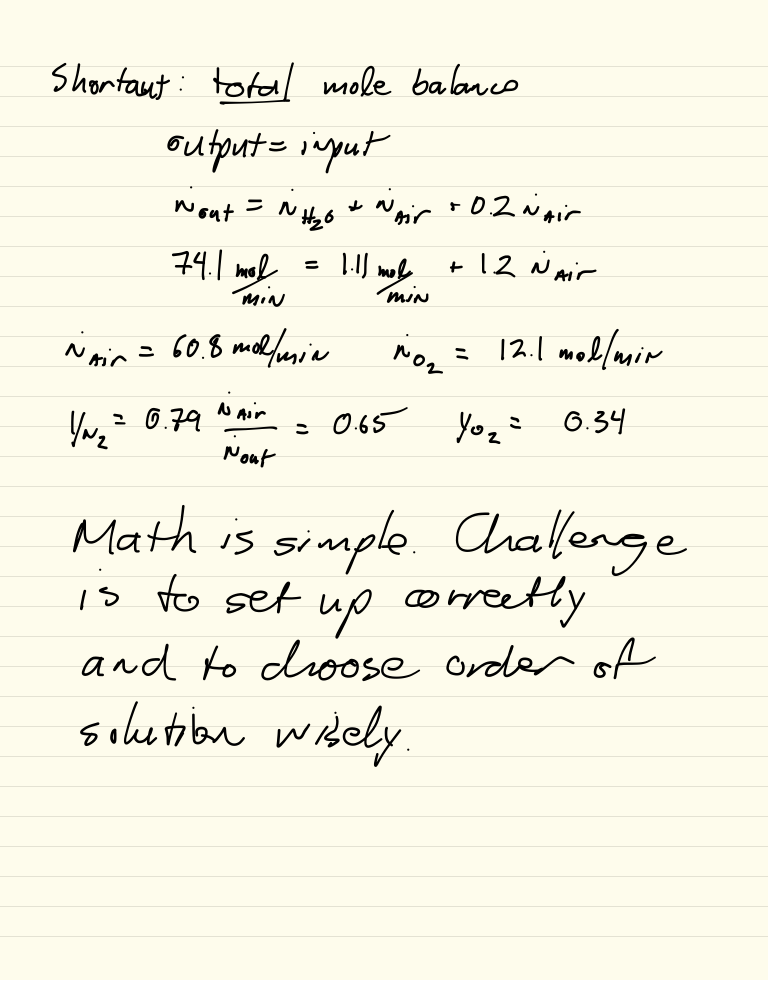
\includegraphics[width=.9\linewidth]{./figs/Diff-balance4.png}

\begin{itemize}
\item Number of equations = number of unknowns.  Say \emph{degrees of freedom} = 0.
\end{itemize}

\begin{quote}
\textbf{EXAMPLE} DOF analysis. Humid air passes through a condenser that removes 95\% of \ce{H2O}. Condensate removed at 225 L/min.  Calculate flow rate and composition of gas stream leaving condenser.
\end{quote}

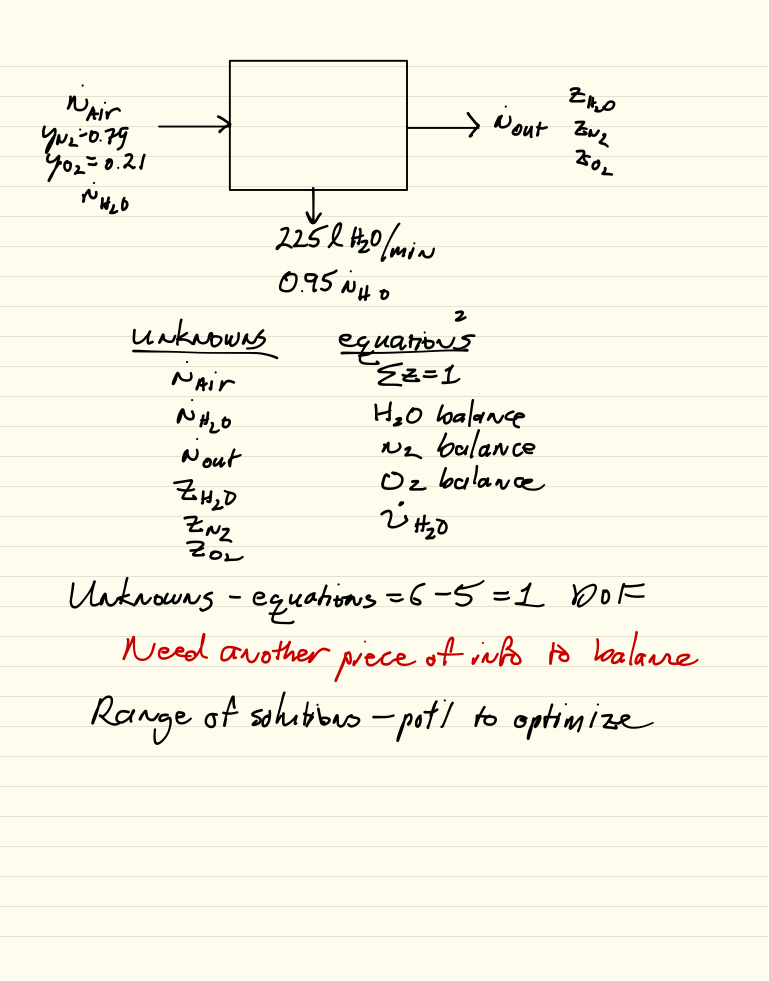
\includegraphics[width=.9\linewidth]{./figs/DOF.png}

\begin{quote}
\textbf{EXAMPLE} 45.0\%(w/w) benzene and balance toluene are fed to a distillation column.  The overhead product contains 95.0\%(mol/mol) benzene and accounts for 92\% of total fed benzene.  The fed enters at 2000 L/h and has specific gravity 0.872.  Determine mass flow rates of overhead and bottom streams and bottom composition.
\end{quote}

\begin{minted}[frame=lines,fontsize=\scriptsize,linenos]{python}
# Convert stream 2 to mass basis
MWb = 6 * 12.0 + 6 * 1.008
MWt = 7 * 12.0 +8 * 1.008
x2B = 0.95
x2T = 0.05

basis = 100.
m2B = basis * x2B * MWb
m2T = basis * x2T * MWt
m2tot = m2B + m2T

z2B = m2B/m2tot
z2T = m2T/m2tot
print('Z2Benzene = {0:5.3f} Z2Toluene = {1:5.3f} kg/kg'.format(z2B,z2T))

# total mass flow rate
SG = 0.872
v1 = 2000  # l/h
m1 = v1 * SG

# benzene flow rates
z1B = 0.45
m3B = 0.08 * m1 * z1B
m2B = 0.92 * m1 * z1B

print('Mdot1 = {0:6.1f}  Mdot2B = {1:6.1f}   Mdot3B = {2:6.1f} kg/hr'.format(m1,m2B,m3B))

# mass balances
m2 = m2B/z2B
m3 = m1 - m2
print('Mdot2 = {0:6.1f}  Mdot3 = {1:6.1f} kg/hr'.format(m2,m3))

# last gasp
z3B = m3B/m3
print('Z3Benzene = {0:5.3f}  Z3Toluene = {1:5.3f} kg/kg'.format(z3B,1-z3B))
\end{minted}

\begin{verbatim}
Z2Benzene = 0.942 Z2Toluene = 0.058 kg/kg
Mdot1 = 1744.0  Mdot2B =  722.0   Mdot3B =   62.8 kg/hr
Mdot2 =  766.8  Mdot3 =  977.2 kg/hr
Z3Benzene = 0.064  Z3Toluene = 0.936 kg/kg
\end{verbatim}

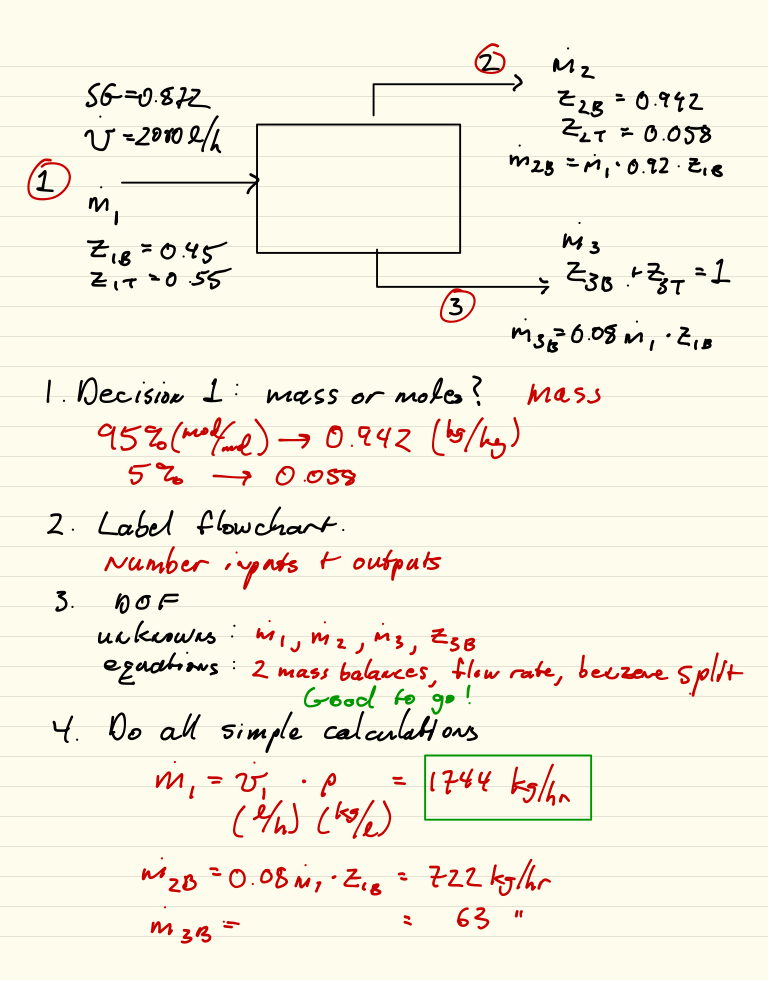
\includegraphics[width=0.8\textwidth]{./figs/Diff-balance5.png}

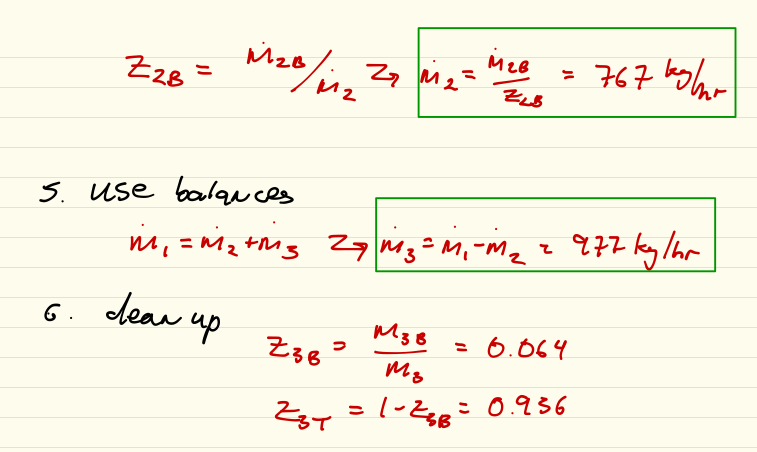
\includegraphics[width=0.8\textwidth]{./figs/Diff-balance6.png}

\begin{quote}
\textbf{EXAMPLE} Integral balance on semi-batch, non-steady state process.  Air is bubbled through a tank of liquid hexane at a rate of 0.100 kmol/min.  The gas stream leaving the tank contains 10.0\%(mol/mol) hexane vapor.
The air is essentially insoluble in hexane.  Estimate the time required to vaporize \SI{10}{\meter\cubed} of the liquid.
\end{quote}

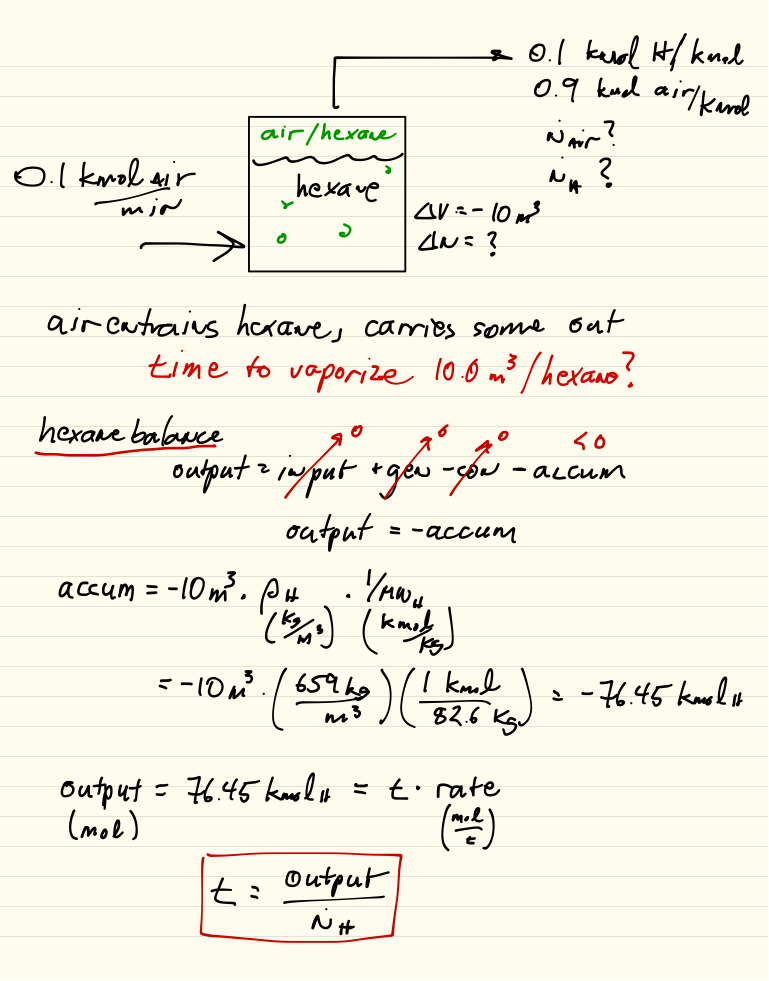
\includegraphics[width=0.8\textwidth]{./figs/Int-balance1.png}

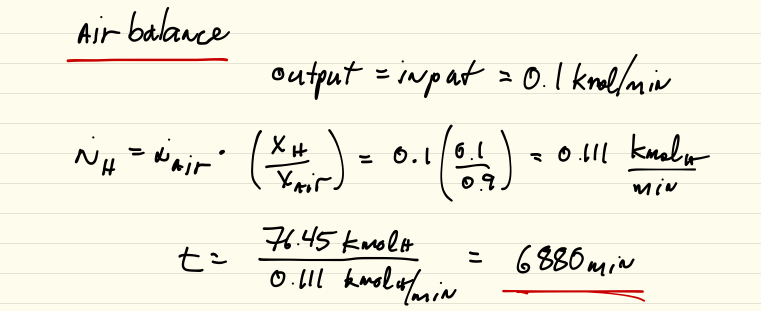
\includegraphics[width=0.8\textwidth]{./figs/Int-balance2.png}

\begin{itemize}
\item Does life always balance?  No!
\end{itemize}

\subsection{Multi-unit processes}
\label{sec-5-4}
\begin{itemize}
\item Real processes will contain multiple sub-processes
\item Can write a balance on any portion we can draw a box around
\end{itemize}

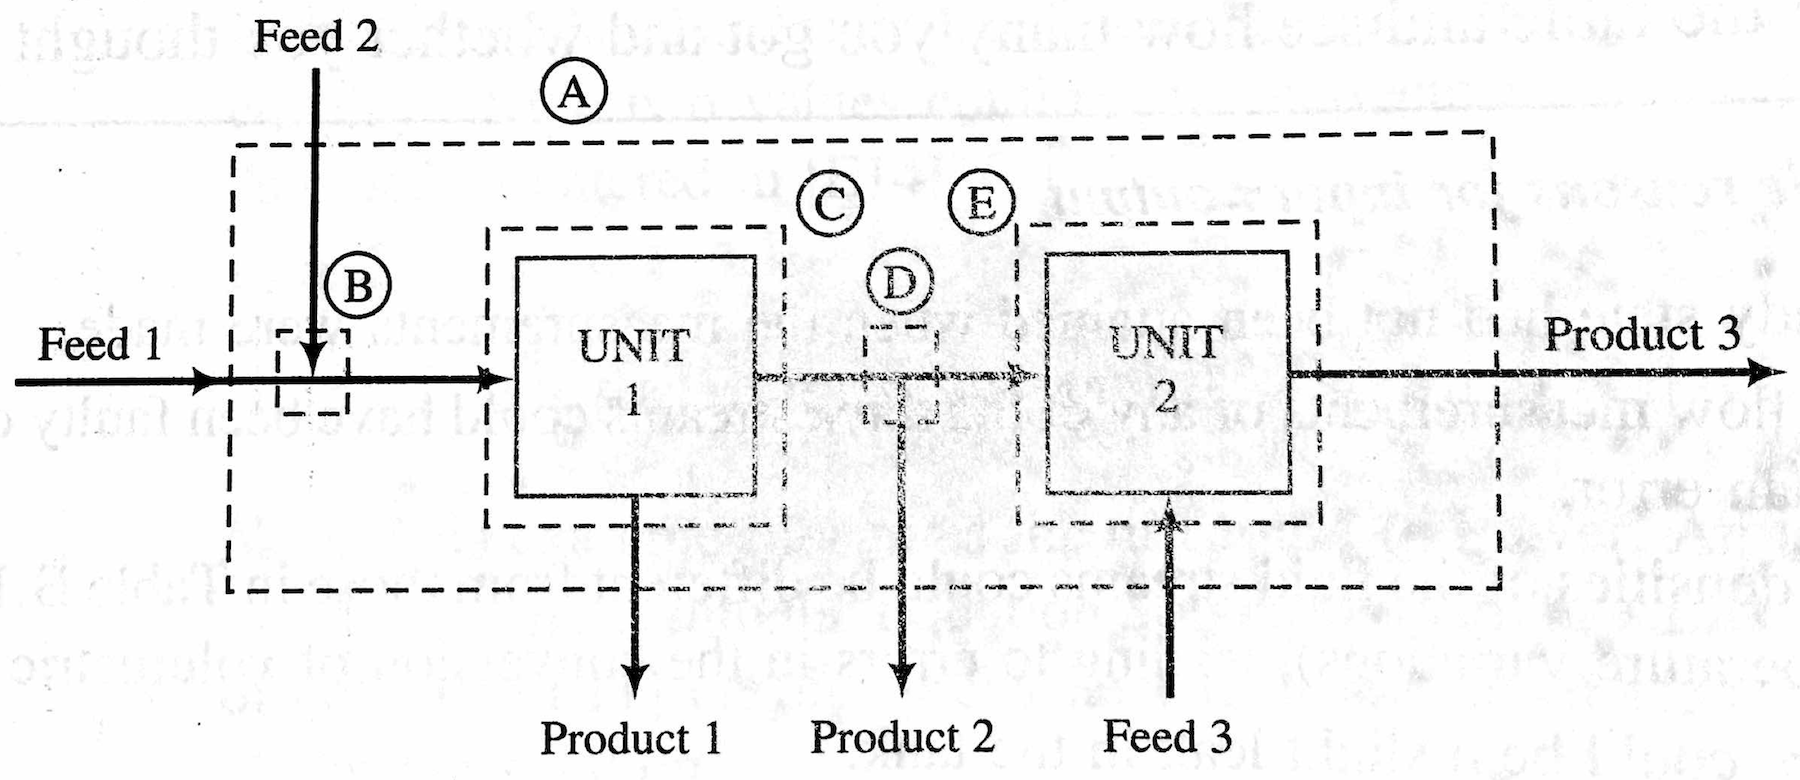
\includegraphics[width=0.8\textwidth]{./figs/Multiprocess.png}

\begin{quote}
\textbf{EXAMPLE} The flow chart below is for a two step, steady-state process involving components A and B.  Find the unknown flow rates.
\end{quote}

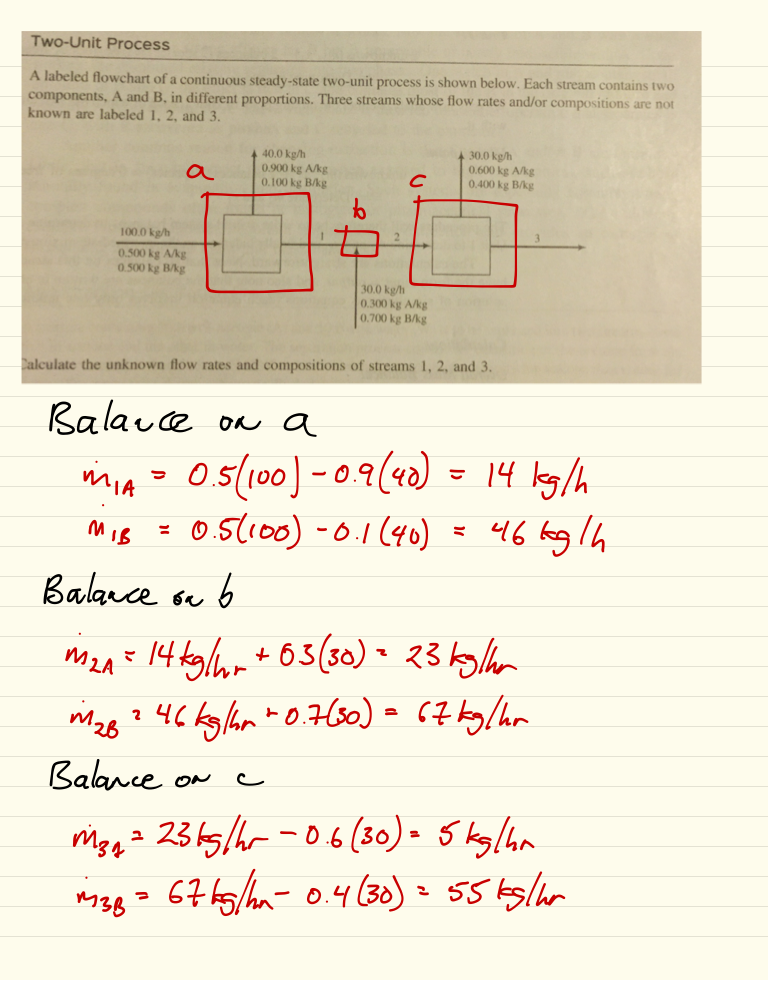
\includegraphics[width=0.8\textwidth]{./figs/Two-unit-soln.png}

\begin{quote}
\textbf{EXAMPLE} Multi-stage extraction-distillation.
\end{quote}

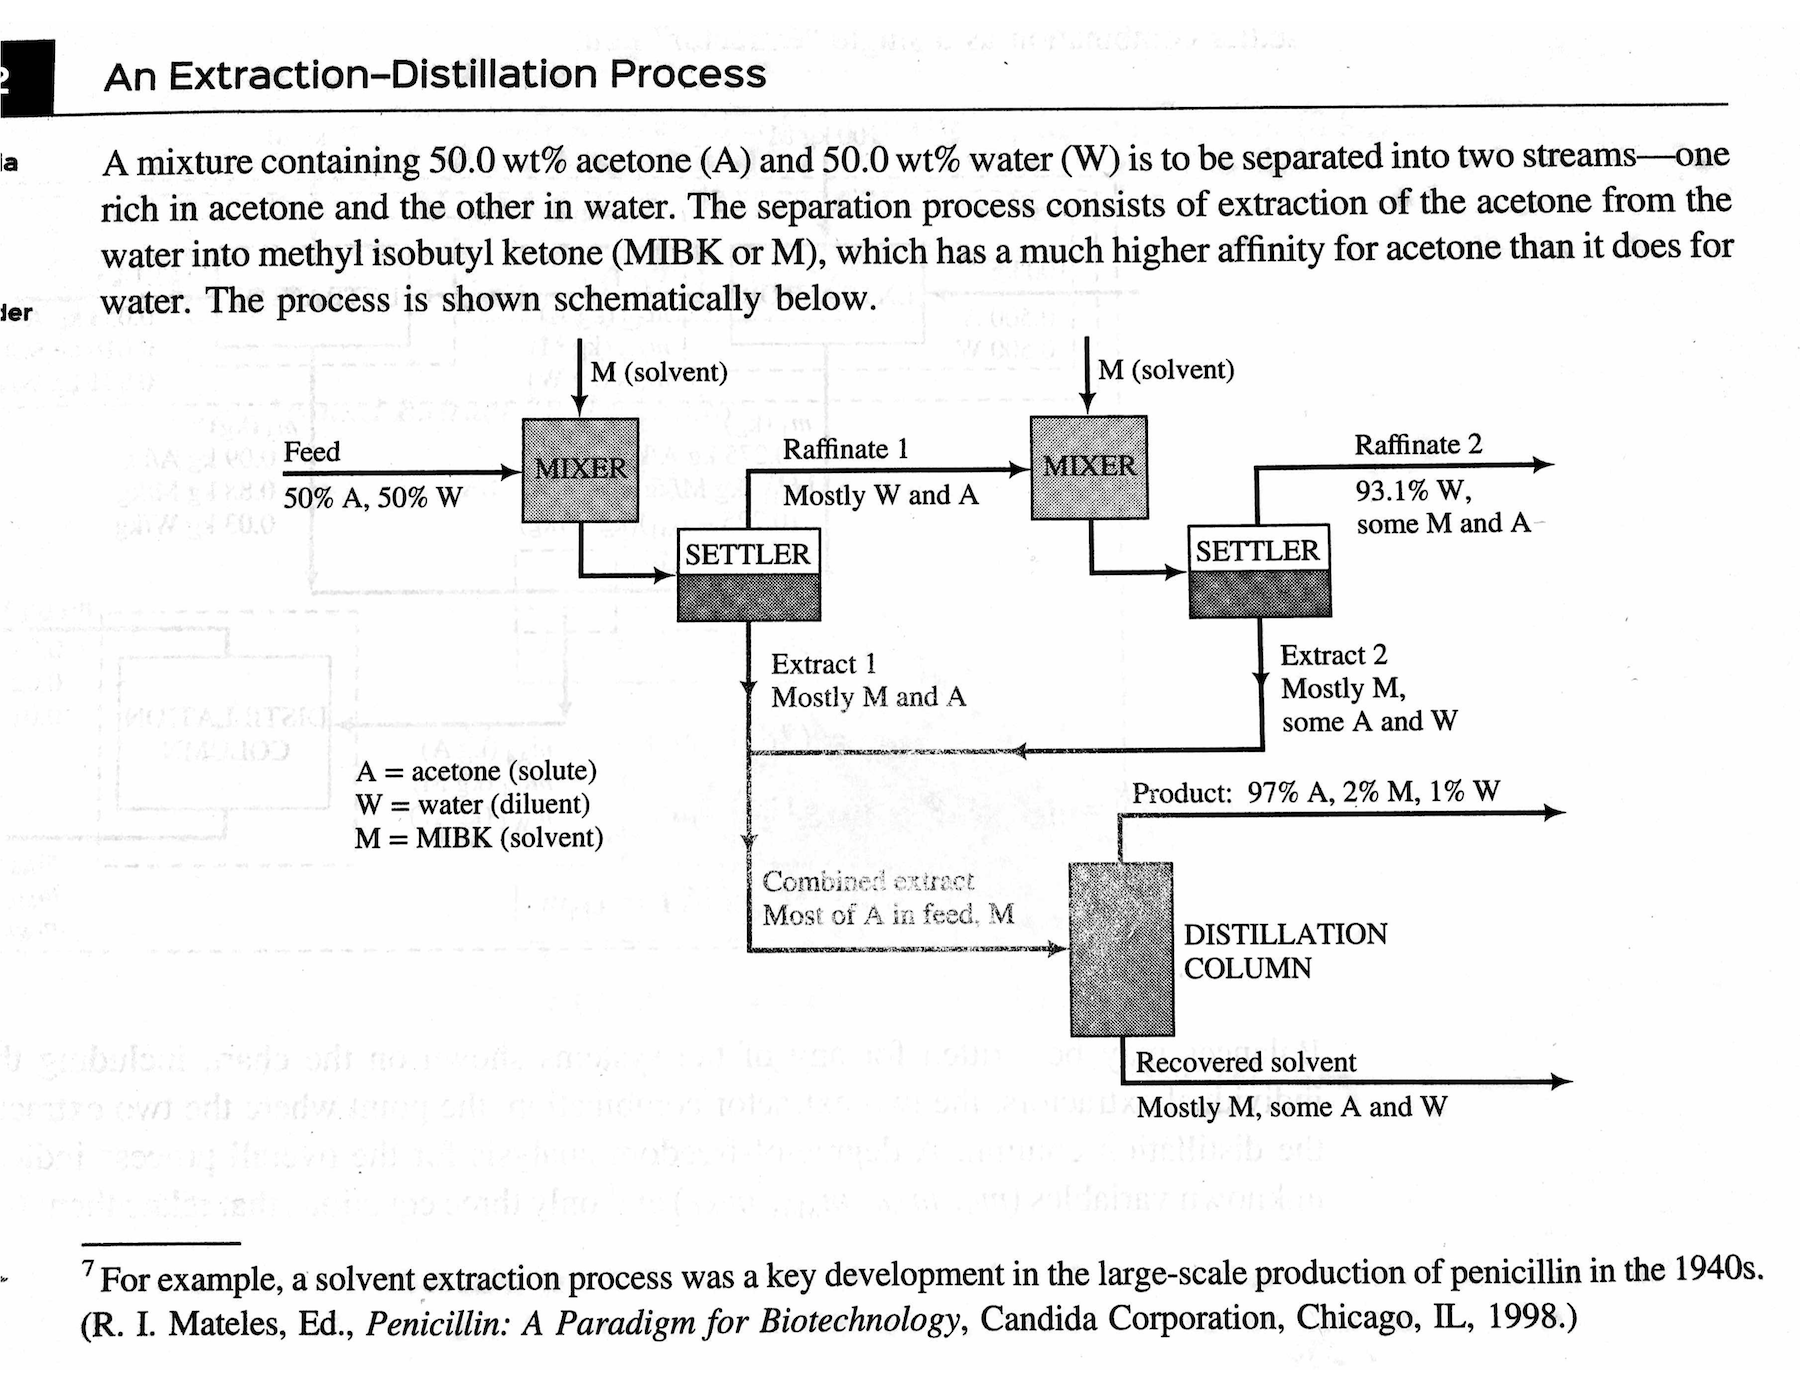
\includegraphics[width=0.8\textwidth]{./figs/Example442.png}

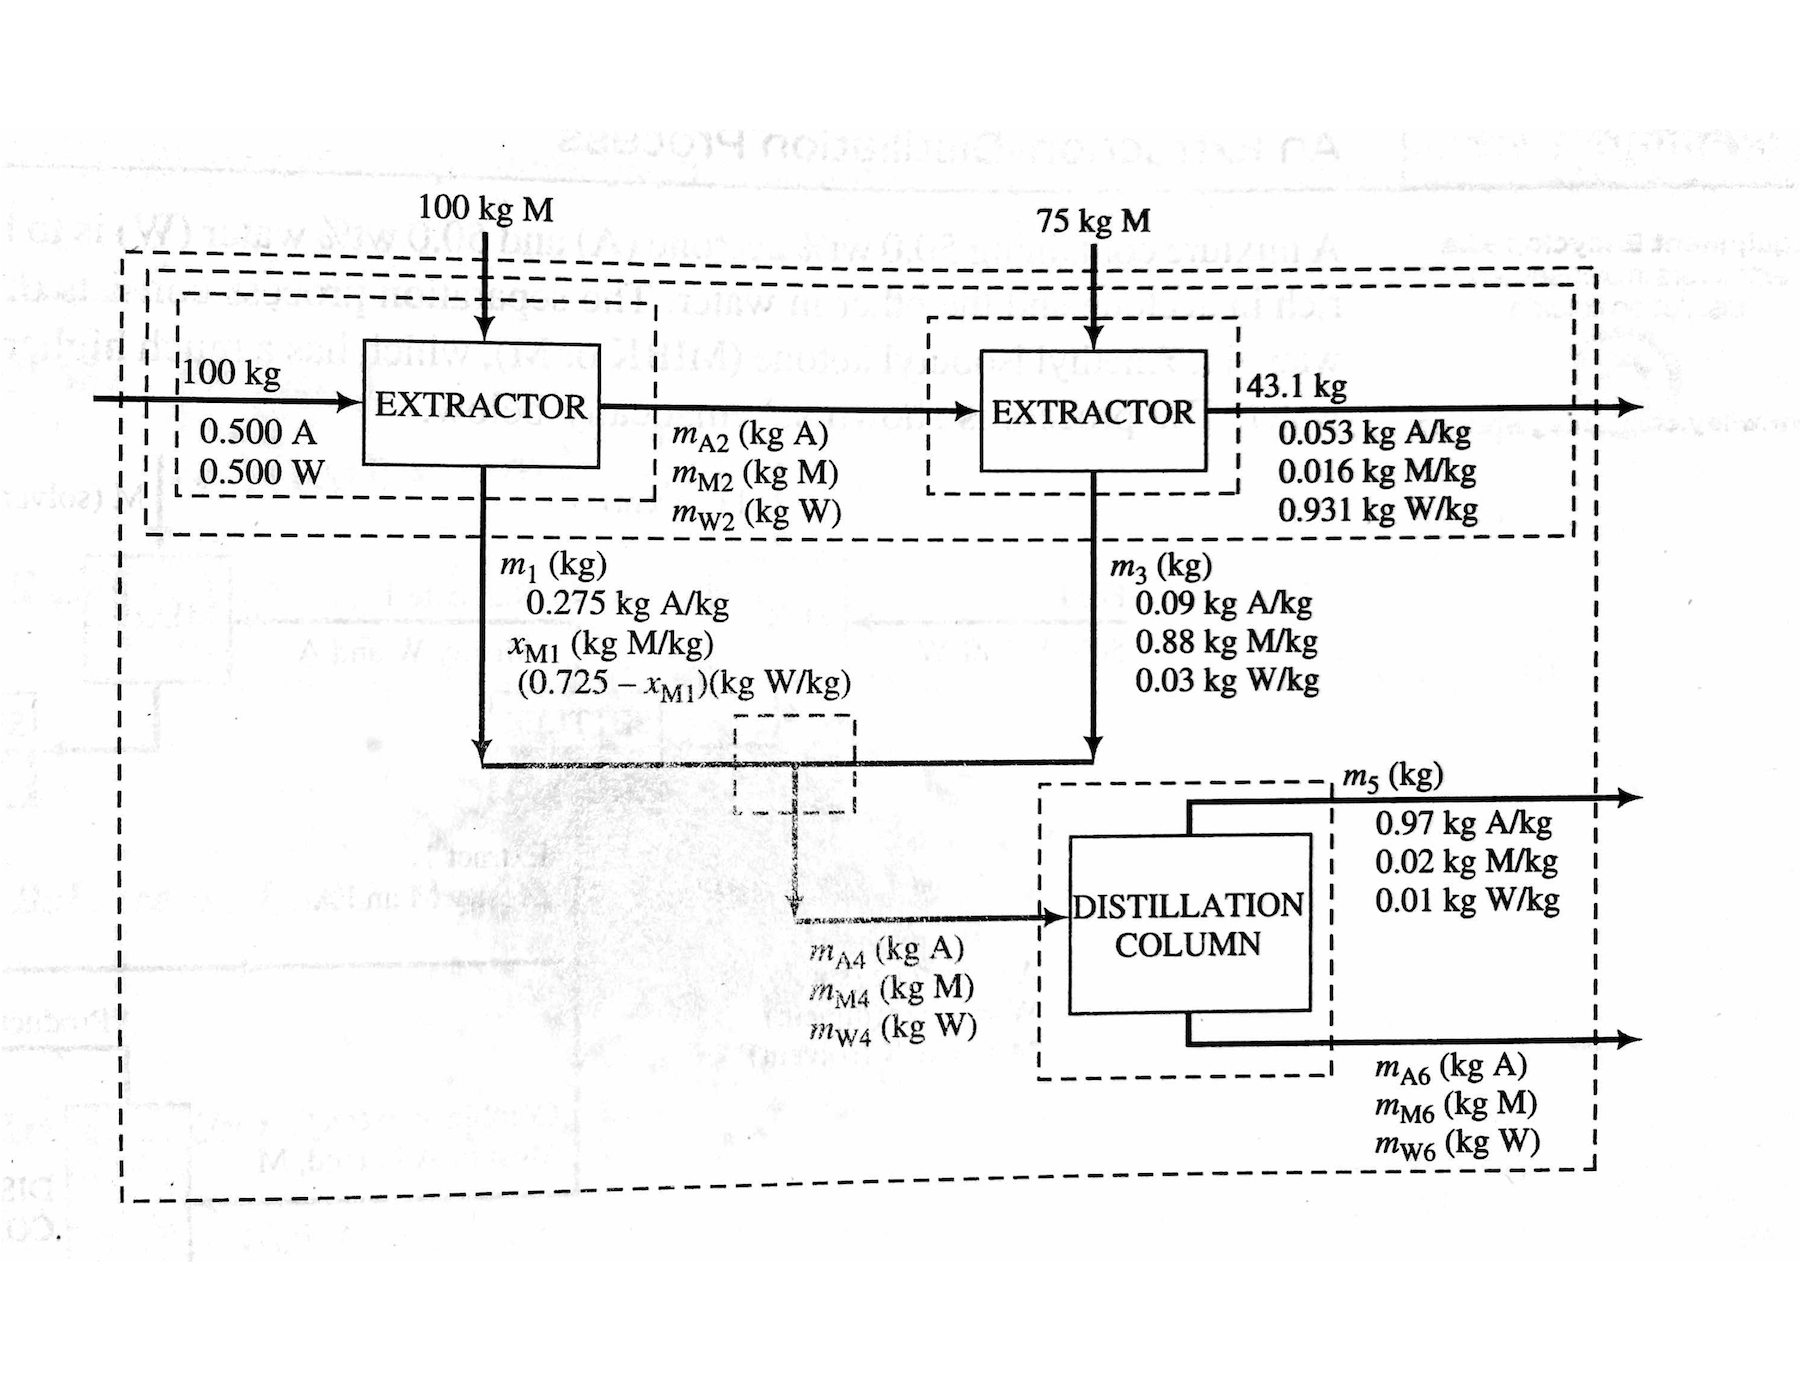
\includegraphics[width=0.8\textwidth]{./figs/Soln442.png}

\begin{itemize}
\item Balance extractor pair
\begin{itemize}
\item Three unknowns
\item Total mass + A balance: \(\dot{m}_1 = 145, \dot{m}_{2} = 86.8\)
\item M balance: \(x_{M1} = 0.675 \)
\end{itemize}
\item Balance extractors individually
\item Balance mixing point
\begin{itemize}
\item \( \dot{m}_{A4} = 86.8, \dot{m}_{M4}= 174, \dot{m}_{W4}= 9.9\)
\end{itemize}
\item Balance column: 4 unknowns, 3 balances $\to$ under-determined
\end{itemize}

\subsection{Recycle and bypass}
\label{sec-5-5}
\begin{itemize}
\item \emph{Recycle} and \emph{bypass} are ways to control the composition in a process
\item \emph{Recycle} a way to recover and re-feed unused reactants
\item Changes effective residence time in the process
\end{itemize}

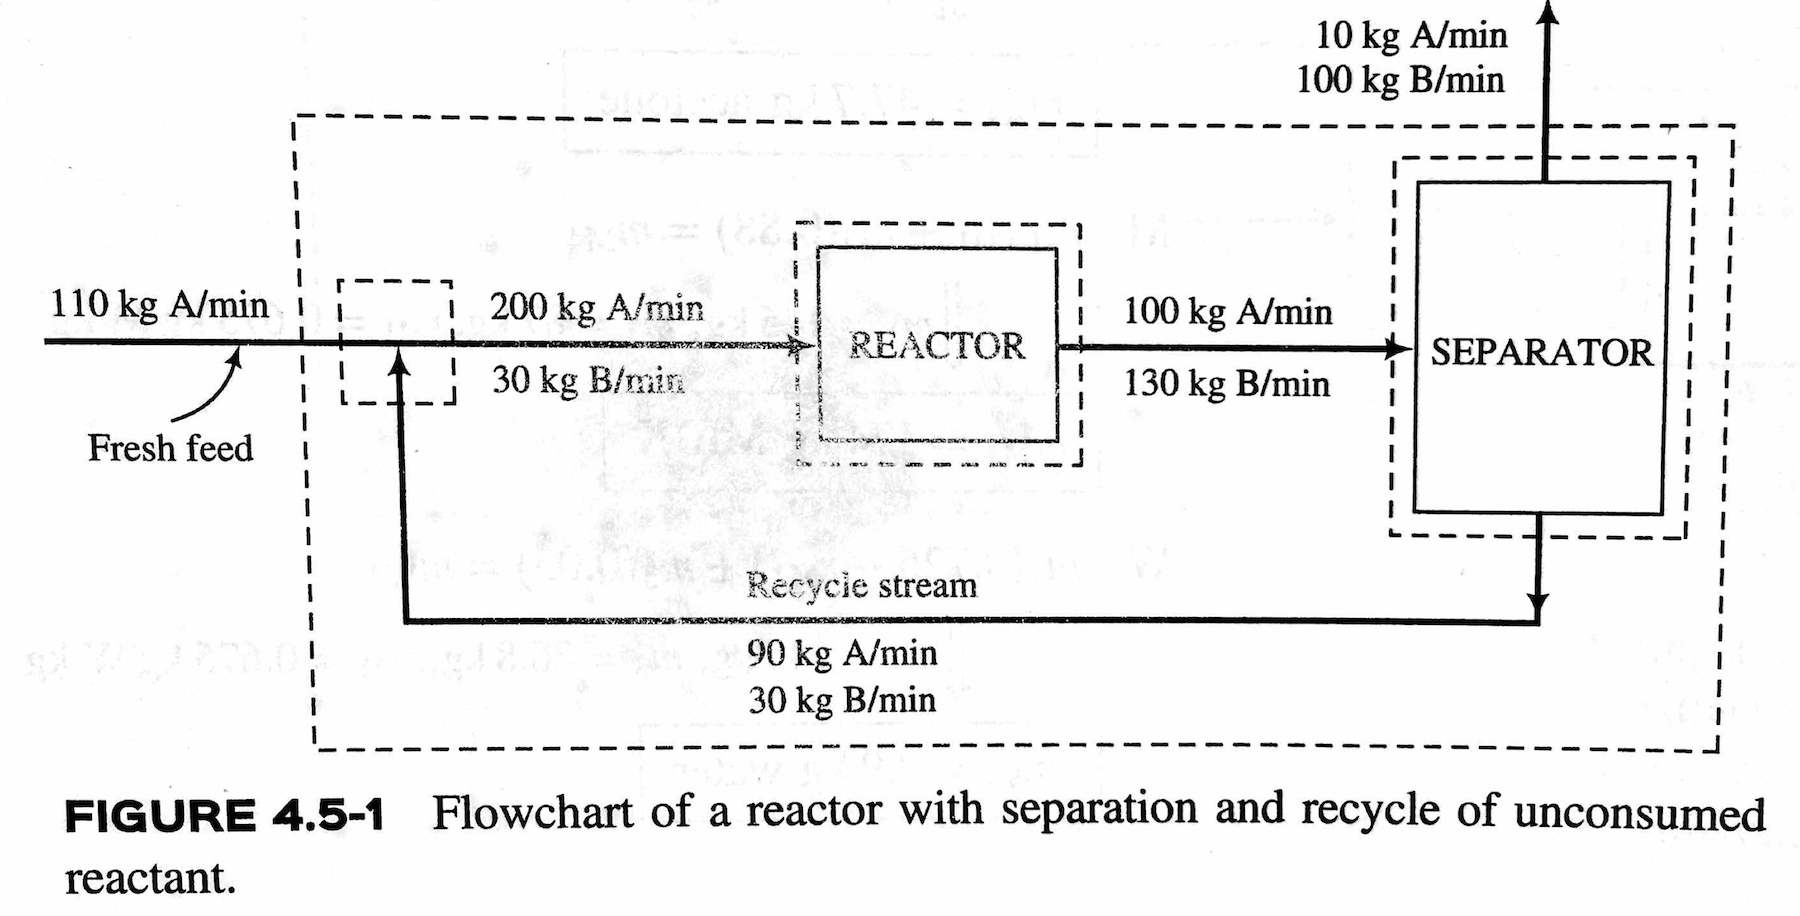
\includegraphics[width=0.8\textwidth]{./figs/Recycle1.png}

\begin{quote}
\textbf{EXAMPLE} Fresh, humid air, 4\% \ce{H2O}, is to be cooled and dehumidified to 1.7\%.  Some of the dehumidified air leaving the air conditioner is recycled into the inlet air.  The blended stream is 2.30\% \ce{H2O}.  Water leaves as pure water.  Find all flow rates.
\end{quote}

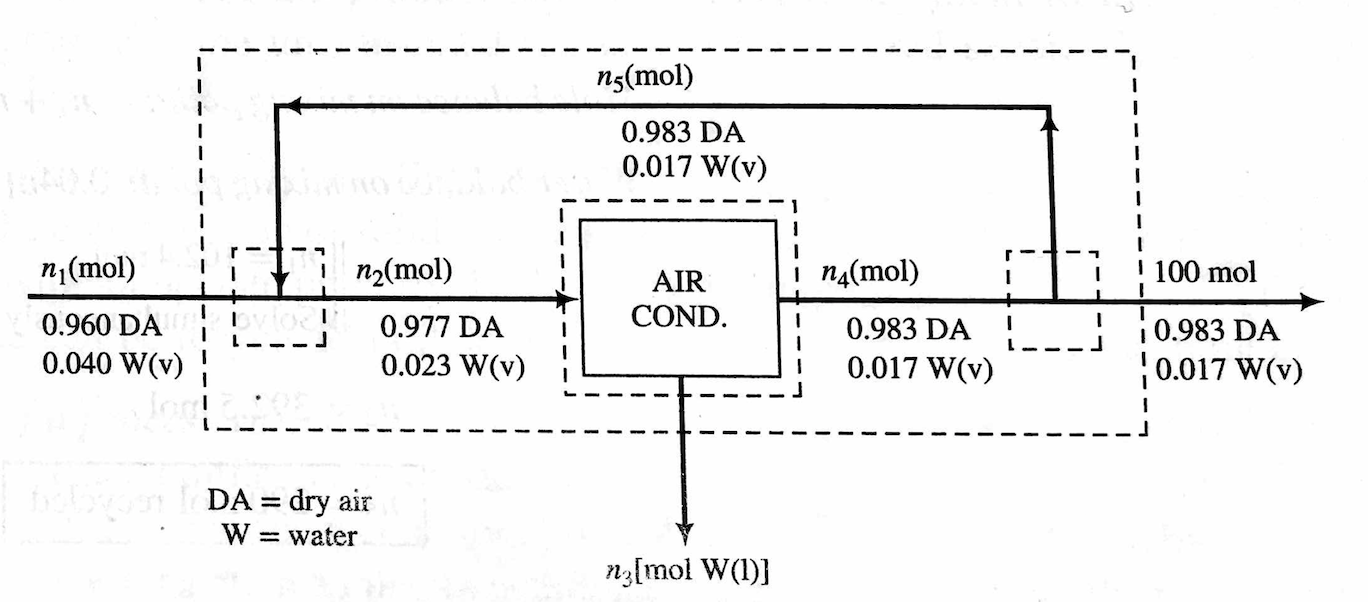
\includegraphics[width=0.8\textwidth]{./figs/Recycle2.png}

\begin{itemize}
\item Mass or moles?
\item Basis? 100 mol/s outlet.
\item Overall balance
\begin{itemize}
\item \(\dot{n}_{1} = 102.4,\quad\dot{n}_{3} = 2.4\)
\end{itemize}
\item Mixing point balance
\begin{itemize}
\item \(\dot{n}_{2} = 392.5,\quad\dot{n}_{5}=290\)
\end{itemize}
\item Split point balance
\begin{itemize}
\item \(\dot{n}_{4} = 100 + \dot{n}_{5} = 390\)
\end{itemize}
\end{itemize}
\newpage

\section{Material balances on reactive systems}
\label{sec-6}
\subsection{Revision idea}
\label{sec-6-1}
\begin{itemize}
\item First introduce balance using single reaction and molecular balance
\item Then introduce extent
\item Then multiple reactions\ldots{}
\end{itemize}
\subsection{Stoichiometry}
\label{sec-6-2}
\begin{itemize}
\item Chemical reaction: a transformation between between chemical species
\begin{itemize}
\item Conserves \emph{mass} and \emph{atom numbers}
\item Isomerization (e.g. \emph{cis}- \emph{trans}) \ce{A <=>B},
\item Condensation (e.g. add \ce{H2O} to double bond) \ce{A+B <=> C}
\item Combustion (e.g. methane) \ce{A + 2B -> C + 2 D}
\end{itemize}
\item Each has a distinct \emph{stoichiometry} that guarantees atom and mass conservation
\item Tells us \emph{ratio} consumption/generation
\end{itemize}

\begin{quote}
\hline
\textbf{EXAMPLE} Balance SCR reaction.  Engine emits 0.02 mol NO/mile.  How many grams \ce{NH3} needed/mile?

\ce{4 NH3 + 4 NO +  O2 -> 4 N2 + 6 H2O}
\hline
\end{quote}


\begin{itemize}
\item Reaction short-hand: species \emph{j} $\to$ \(A_{j}\)
\item Stoichiometric coefficient:
\end{itemize}

\begin{equation*}
\nu_{j}= \left\{
\begin{array}{rl}
< 0 & \text{reactant}\\
> 0 & \text{product}
\end{array}
\end{equation*}
\begin{equation*}
\sum_{j} \nu_{j} A_{j} = 0
\end{equation*}

\begin{itemize}
\item Can scale by arbitrary constant \emph{c}
\end{itemize}
\subsection{Reaction progress}
\label{sec-6-3}
\begin{itemize}
\item Stoichiometry tells us how moles of reactants/products vary along course of reaction
\end{itemize}

\begin{quote}
\textbf{EXAMPLE} \ce{A -> B}.  Total moles conserved:
\begin{eqnarray*}
n_{tot} & = & n_{A0} + n_{B0} = n_{A} + n_{B}\\
n_{B} & = & n_{tot} - n_{A}
\end{eqnarray*}

Plot \(n_{B}\) vs. \(n_{A}\).
\end{quote}

\begin{itemize}
\item Illustrate ``ICE'' procedure for SCR reaction
\item Reaction advancement/extent $\xi$:
\end{itemize}

\begin{equation*}
n_{j} = n_{j0} + \nu_{j} \xi
\end{equation*}

\begin{itemize}
\item we define $\xi$ to be extensive, units of ``moles'' or ``moles/time''
\end{itemize}

\begin{quote}
\hline
\textbf{EXAMPLE} Stoichiometric SCR mixture.  Plot moles of each species as a function of advancement.
\hline
\end{quote}
\begin{minted}[frame=lines,fontsize=\scriptsize,linenos]{python}
import matplotlib.pyplot as plt
import numpy as np

nu = np.array([[-4, -6, -3, 5, 6]])
n0 = np.array([[4, 6, 3, 0, 0]])

xi = np.array([np.linspace(0,1)])

n = np.transpose(n0) + np.dot(np.transpose(nu),xi)

for i in range(5):
    plt.plot(xi[0],n[i])

plt.savefig('./figs/advancement1.png')
\end{minted}

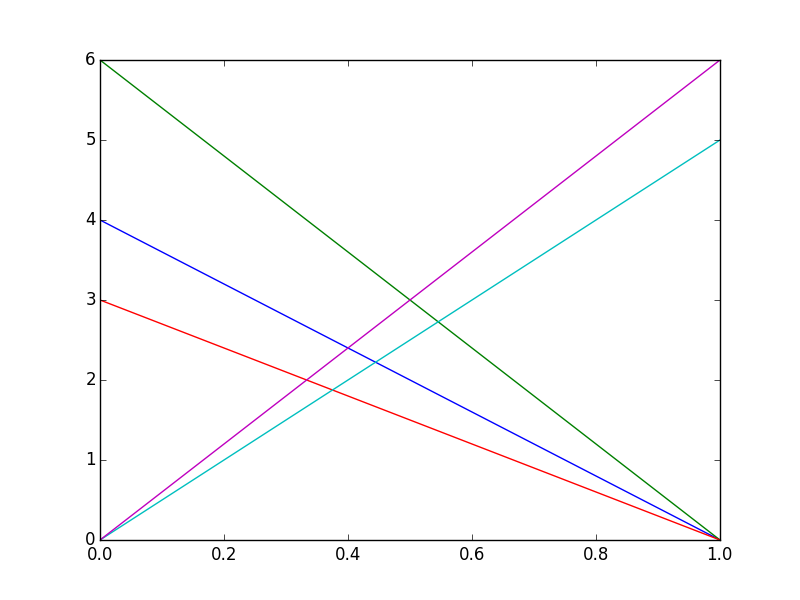
\includegraphics[width=0.8\textwidth]{./figs/advancement1.png}


\begin{itemize}
\item Must have \(n_{j} \ge 0\) for all \emph{j}, or \( \xi \le -\frac{n_{j0}}{\nu_{j}}\):
\end{itemize}

\begin{eqnarray*}
\text{Forward: } \xi_{max} & =  & \min_\text{reactants} \left ( -\frac{n_{j0}}{\nu_{j}}\right ) \\
\text{Reverse: } \xi_{min} & = & \max_\text{products}\left (-\frac{n_{j0}}{\nu_{j}} \right )
\end{eqnarray*}

\begin{equation*}
\xi_{min} \le \xi \le \xi_{max}
\end{equation*}

\begin{quote}
\hline
Air oxidation of \ce{NH3}.

\ce{4 NH3 + 5 O2 -> 4 NO + 6 H2O}

0.1 g/s \ce{NH3} and 0.95 g/s air flow into a reactor.  What is limiting reagent?  How much \ce{NH3} at completion?
\hline
\end{quote}

\begin{minted}[frame=lines,fontsize=\scriptsize,linenos]{python}
MWNH3 = 17; MWO2 = 32; MWN2 = 28;
MWair = 0.79 * MWN2 + 0.21 * MWO2

mNH30 = 0.1; mair0 = 0.95
nNH30 = mNH30 / MWNH3
nO20 = (mair0 / MWair) * 0.21

print('ndot NH3 = {0:6.4f}  ndot O2= {1:6.4f} mol/s\n'.format(nNH30,nO20))

nuNH3 = -4.0; nuO2 = -5.0;

xiNH3 = -nNH30/nuNH3; xiO2 = -nO20/nuO2

print('ndot/nu NH3 = {0:7.5f}  ndot/nu O2 = {1:7.5f}\n'.format(xiNH3,xiO2))

print('O2 limiting\n')

xilim = xiO2

nNH3 = nNH30 + nuNH3 * xilim; nO2 = nO20 + nuO2 *xilim

print('ndot NH3 = {0:7.5f}  ndotO2 = {1:7.5f}\n'.format(nNH3,nO2))

fNH3 = 100*(nNH30 - nNH3)/nNH30
print('Fraction NH3 consumed = {0:4.2f}%'.format(fNH3))
\end{minted}

\begin{verbatim}
ndot NH3 = 0.0059  ndot O2= 0.0069 mol/s

ndot/nu NH3 = 0.00147  ndot/nu O2 = 0.00138

O2 limiting

ndot NH3 = 0.00035  ndotO2 = 0.00000

Fraction NH3 consumed = 94.08%
\end{verbatim}

\begin{itemize}
\item \emph{conversion} often used to measure consumption of a species:
\end{itemize}

\[X_{j} = \frac{n_{j0}-n_{j}}{n_{j0}} = -\frac{\nu_{j}\xi}{n_{j0}} \]

\begin{itemize}
\item conventional to define ``the'' conversion in terms of limiting reagent:
\end{itemize}

\[X = 1 - \frac{n_{\text{lim}}}{n_{\text{lim},0}} = -\frac{\nu_{j}\xi}{n_{j0}} \]

\[ \xi = -X \frac{n_{\text{lim},0}}{\nu_{\text{lim}}} \]

\begin{itemize}
\item \emph{X} is unitless and (for forward reaction) \( 0 \le X \le 1\)
\item all \(n_{j}\) can be written in terms of \emph{X}:
\end{itemize}

\[n_{j} = n_{j0} - X n_{\text{lim},0} * \frac{\nu_{j}}{\nu_{\text{lim}}}\]

\begin{quote}
\hline
\textbf{EXAMPLE} \ce{NH3} oxidation goes to 50\% completion.  What is composition of exit stream?
\hline
\end{quote}

\begin{minted}[frame=lines,fontsize=\scriptsize,linenos]{python}
import numpy as np
import matplotlib.pyplot as plt

species = ('NH3', 'N2', 'O2', 'NO', 'H2O')
nu = np.array([[-4, 0, -6, 5, 6]])

MWNH3 = 17; MWO2 = 32; MWN2 = 28;
MWair = 0.79 * MWN2 + 0.21 * MWO2

mNH30 = 0.1; mair0 = 0.95
nNH30 = mNH30 / MWNH3
nO20 = (mair0 / MWair) * 0.21
nN20 = (mair0 / MWair) * 0.79

n0 = np.array([[nNH30, nN20, nO20, 0, 0]])

X = 0.5

n = n0 - (nu/nu[0,2]) * n0[0,2] * X

print(species)
print(n,' mol/s')

X = np.array([np.linspace(0,1)])

n = np.transpose(n0) - np.dot(n0[0,2]*np.transpose(nu/nu[0,2]),X)

ntot= 0

for i in range(5):
    plt.plot(X[0],n[i],label=species[i])
    ntot =ntot + n[i]
legend = plt.legend()

plt.plot(X[0],ntot)
plt.xlabel('Conversion')
plt.ylabel('flow rate (mol/s)')

plt.savefig('./figs/conversion1.png')
\end{minted}

\begin{verbatim}
('NH3', 'N2', 'O2', 'NO', 'H2O')
[[ 0.00357653  0.02602288  0.00345874  0.00288228  0.00345874]]  mol/s
\end{verbatim}

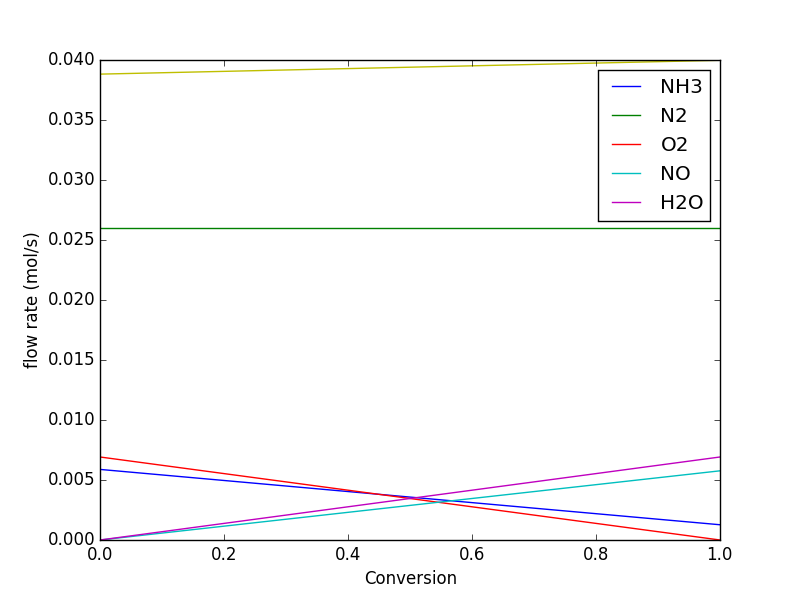
\includegraphics[width=0.8\textwidth]{./figs/conversion1.png}

\subsection{Multiple reactions}
\label{sec-6-4}
\begin{itemize}
\item \ce{NH3} oxidation and SCR together, for example, are parallel reactions
\item competition between the two
\item each species has a stoichiometric coefficient in each parallel reaction
\end{itemize}

\begin{center}
\ce{4 NO + 4 NH3 + O2 -> 4 N2 + 6 H2O} \\
\ce{4 NH3 + 5 O2 -> 4 NO + 6 H2O}\\
\vspace{1em}
\ce{-4 NO  -4 NH3  -1 O2 + 4 N2 + 6 H2O\ = 0} \\
\ce{ 4 NO  -4 NH3  -5 O2 + 0 N2 + 6 H2O}\ = 0\\
\end{center}

\begin{itemize}
\item reaction expression:
\end{itemize}

\begin{equation}
\left (
\begin{array}{rrrrr}
-4 & -4 & -1 & 4 & 6 \\
4 & -4 & -5 & 0 & 6
\end{array}
\right )
\left (
\begin{array}{rr}
A_{1} \\
A_{2} \\
A_{3} \\
A_{4} \\
A_{5}
\end{array}
\right ) = 0
\end{equation}

\begin{itemize}
\item In general \( \sum_{j} \nu_{ij} A_{j} = 0\)

\item each parallel reaction has its own advancement \(\xi_{i}\) (\emph{i} for reactions, \emph{j} for species)
\end{itemize}

\[ n_{j} = n_{j0} + \sum_{i} \nu_{ij} \xi_{i} \]

\begin{itemize}
\item \emph{yield} defined as amount (molar) of desired product over maximum possible amount of desired product

\item \emph{selectivity} (often) defined as amount of desired product over amount of
undesired.  Be careful with this one.
\end{itemize}

\begin{quote}
\hline
\textbf{Selectivity and yield}  Ethane cracking. Feed contains 85.0\% (mol/mol) ethane, balance inerts. 50.1\% of ethane is converted, and ethylene yield is 47.1\%.  Molar composition of gases and selectivity to ethylene?
\begin{center}
\ce{C2H6 -> C2H4 + H2}

\ce{C2H6 + H2 -> 2 CH4}
\end{center}
\hline
\end{quote}

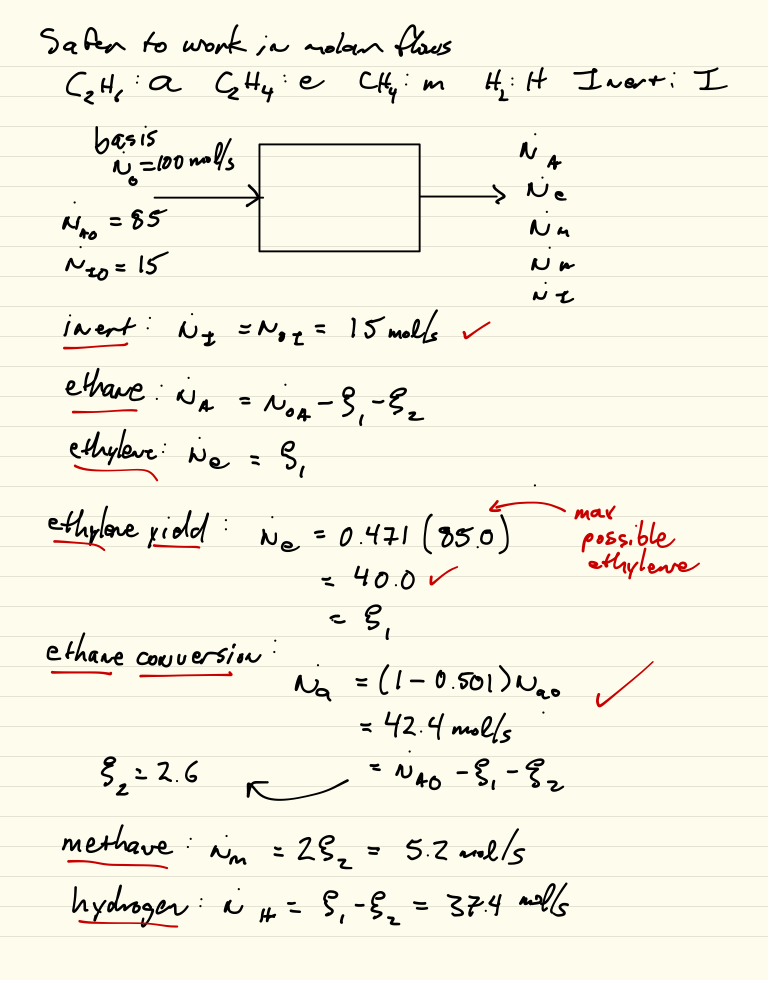
\includegraphics[width=0.8\textwidth]{./figs/Multirxn1.png}

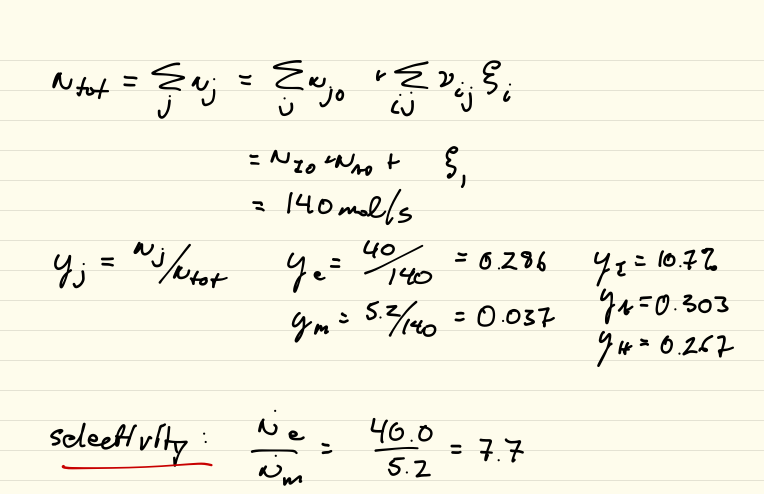
\includegraphics[width=0.8\textwidth]{./figs/Multirxn2.png}

\begin{itemize}
\item DOF analysis: 5 flow rates + 2 reactions - 5 species - 2 constraints = 0 DOFs
\item Example of a balance on a reactive system
\end{itemize}

\subsection{Reactive balances}
\label{sec-6-5}
\begin{itemize}
\item General balance expression:
\end{itemize}
\begin{framed}
output = input + generation - consumption - accumulation
\end{framed}

\begin{itemize}
\item can write balances on \emph{molecular species}:
\end{itemize}

\[ \dot{n}_{A} = \dot{n}_{A0} - \dot{n}_{e} - \frac{1}{2}\dot{n}_{m} \]

\begin{itemize}
\item for more than one reaction, this gets messy

\item extent of reaction
\begin{itemize}
\item each \emph{independent} extent becomes an additional unknown (linearly independent extents)
\item each species balance becomes an equation
\item species balances must include \emph{generation} and \emph{consumption}
\end{itemize}
\end{itemize}

\[\dot{n}_{A} = \dot{n}_{A0} + \sum_{i}\nu_{iA}\xi_{i}\]

\begin{itemize}
\item atomic species
\begin{itemize}
\item one equation for each reactive \emph{atomic species}
\item No generation or consumption;  \emph{input} = \emph{output}
\end{itemize}
\end{itemize}

C balance: \(2 \dot{n_{A0}} = 2 \dot{n_{A}} 2 \dot{n_{e}} + \dot{n_{m}}\)

H balance: \(4 \dot{n}_{A0} = 6\dot{n}_{A} + 4\dot{n}_{e} + 4\dot{n}_{m} + 2\dot{n}_{H} \)

\begin{itemize}
\item one equation for each non-reactive species
\end{itemize}

\begin{quote}
\hline
\textbf{Reactive balances}  Methane is burned in air to make CO and \ce{CO2}:
\begin{center}
\ce{CH4 + 3/2 O2 -> CO + 2 H2O}

\ce{CH4 + 2 O2 -> CO2 + 2 H2O}
\end{center}
Feed contains 7.8\%(mol/mol) \ce{CH4} and balance air (19.4\% \ce{O2}, 72.8\% \ce{N2}).  Methane conversion is 90.0\% and exit contains 8 mol \ce{CO2}/\ce{CO}.  Calculate composition of exit stream.
\hline
\end{quote}

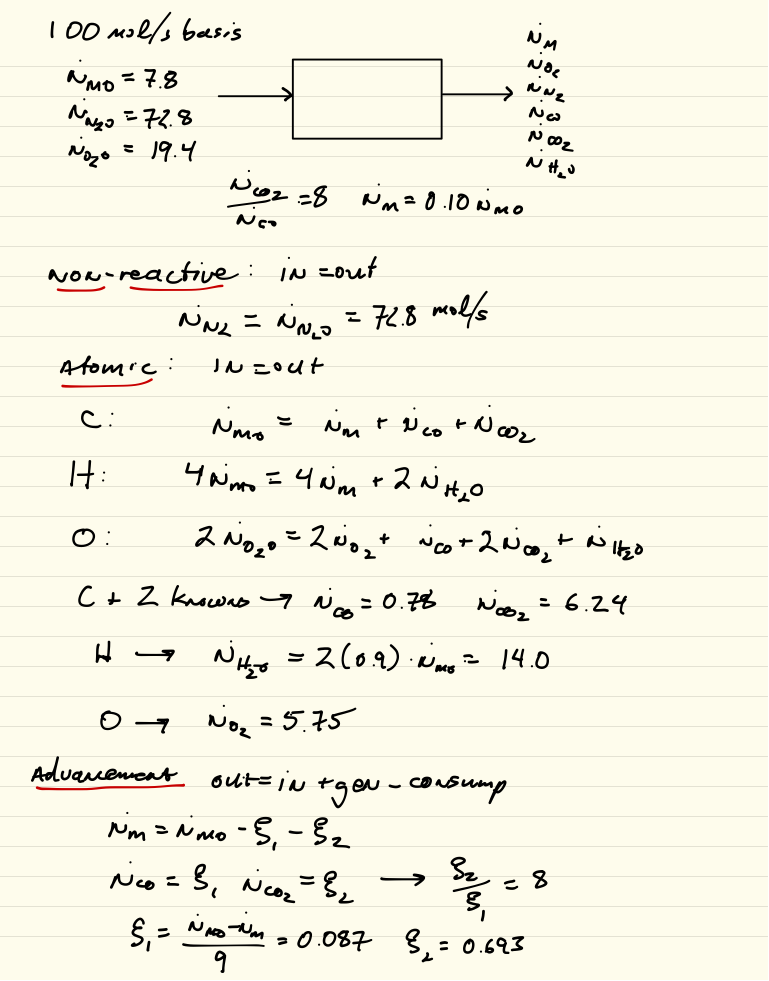
\includegraphics[width=0.8\textwidth]{./figs/Reactive.png}

\subsection{Reactive balances on multi-unit processes}
\label{sec-6-6}
\begin{itemize}
\item Can do extent or atomic balances on any part of a process
\end{itemize}

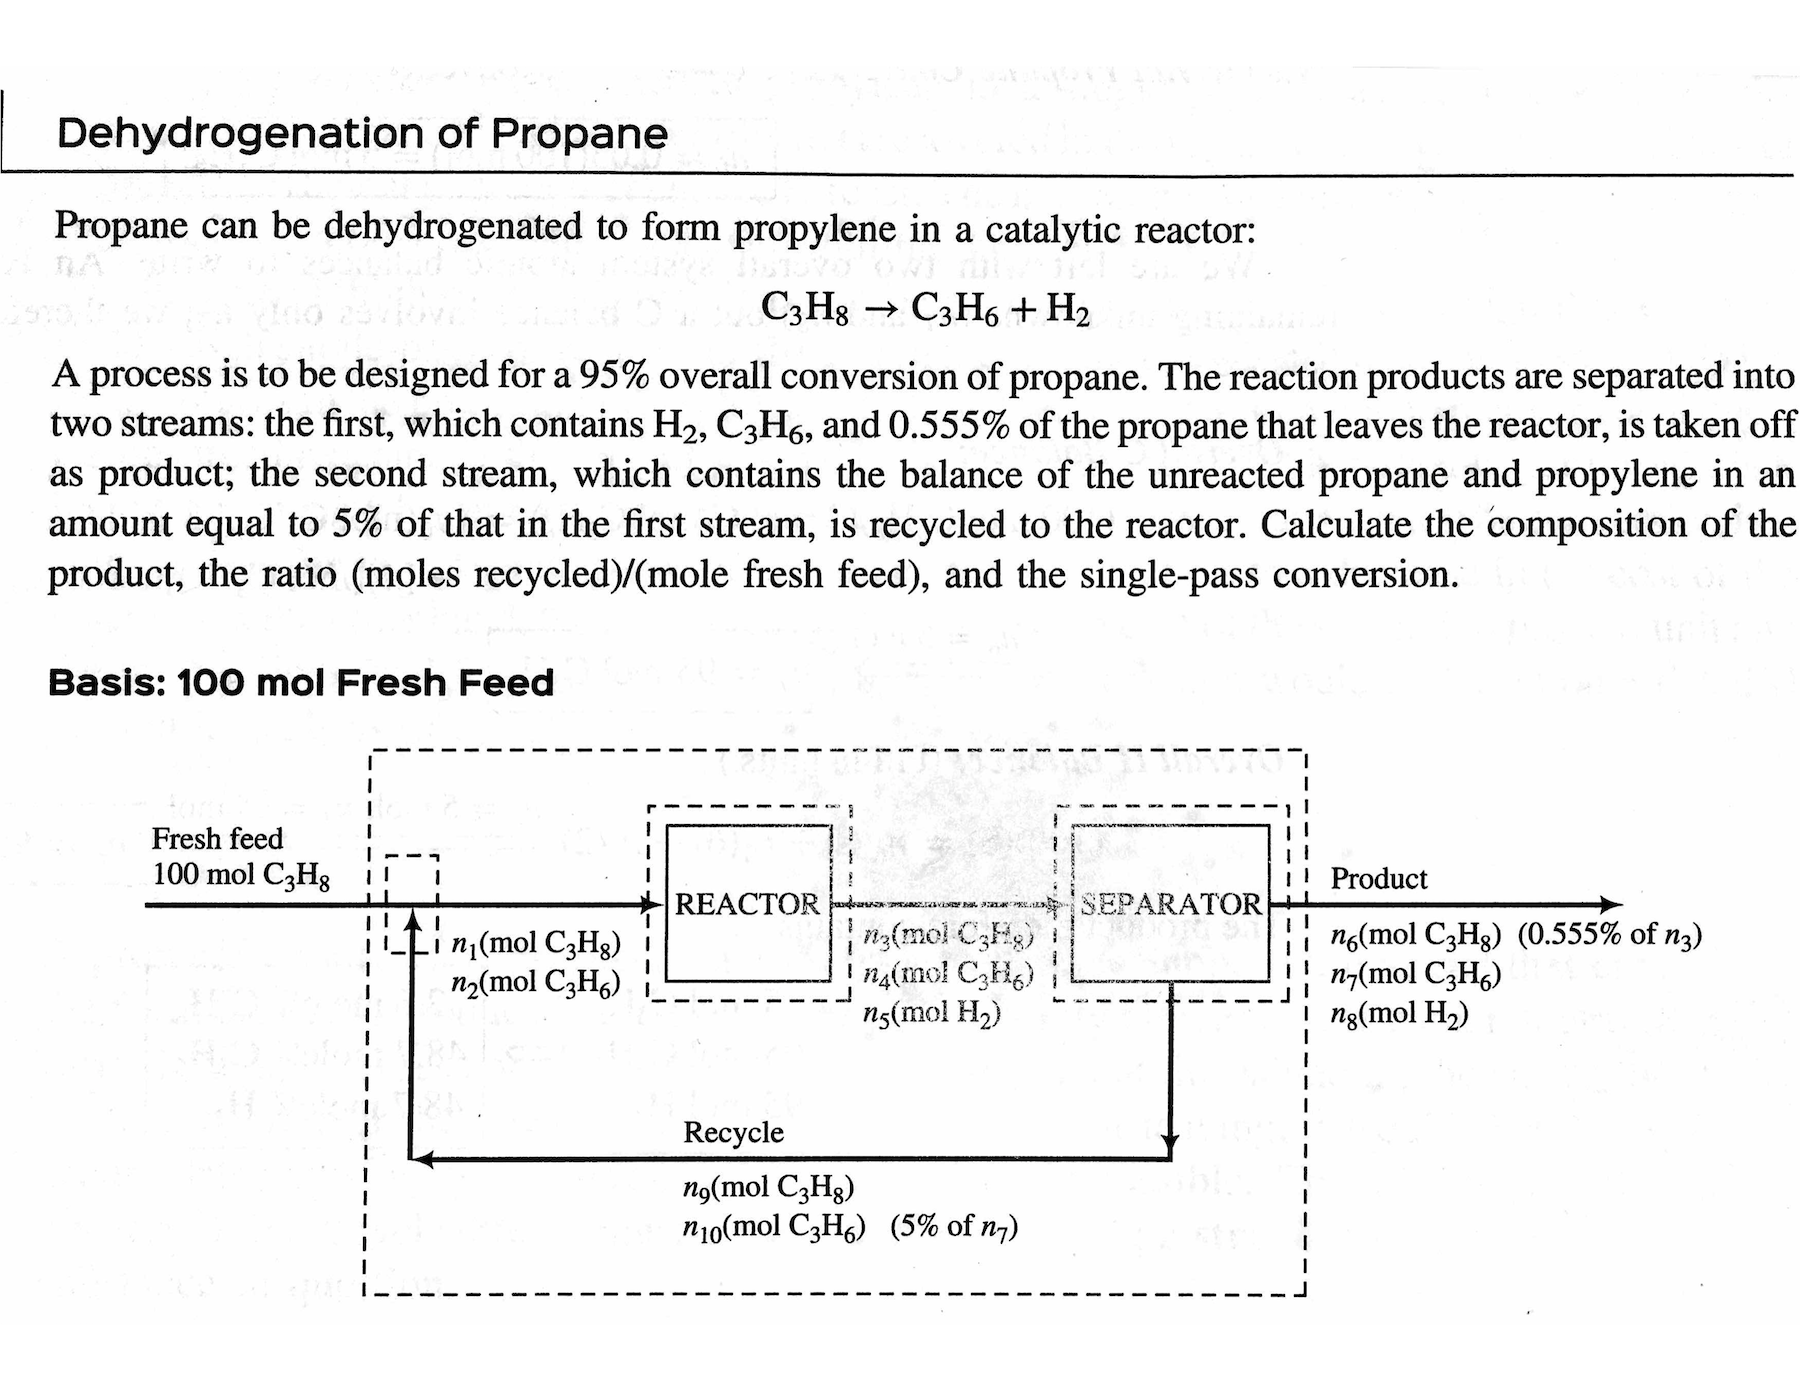
\includegraphics[width=0.8\textwidth]{./figs/Example472.png}

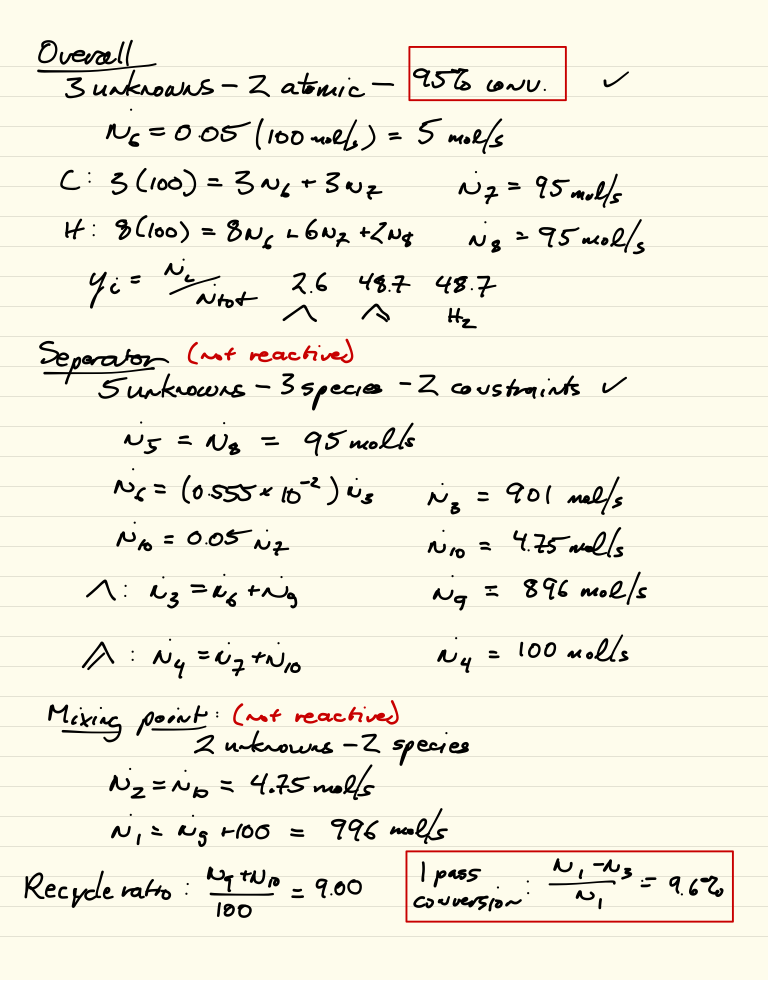
\includegraphics[width=0.8\textwidth]{./figs/ReactiveRecycle.png}

\begin{itemize}
\item Compare single-pass and overall conversion
\item Separation and recycle allows reactor to run at lower conversion at cost of separation unit and larger flows through reactor
\end{itemize}

\subsection{Purge}
\label{sec-6-7}
\begin{itemize}
\item Recycle example above works because system is continuously fed pure reactant
\item If system fed unreactive species, unless it is removed at same rate it enters, it will build up and eventually kill the process
\item Purge stream used to bleed off that species
\end{itemize}

\begin{quote}
\textbf{Purge Example}  \ce{CO2} to methanol.  Single pass 60.0\% \ce{H2} conversion.
\end{quote}
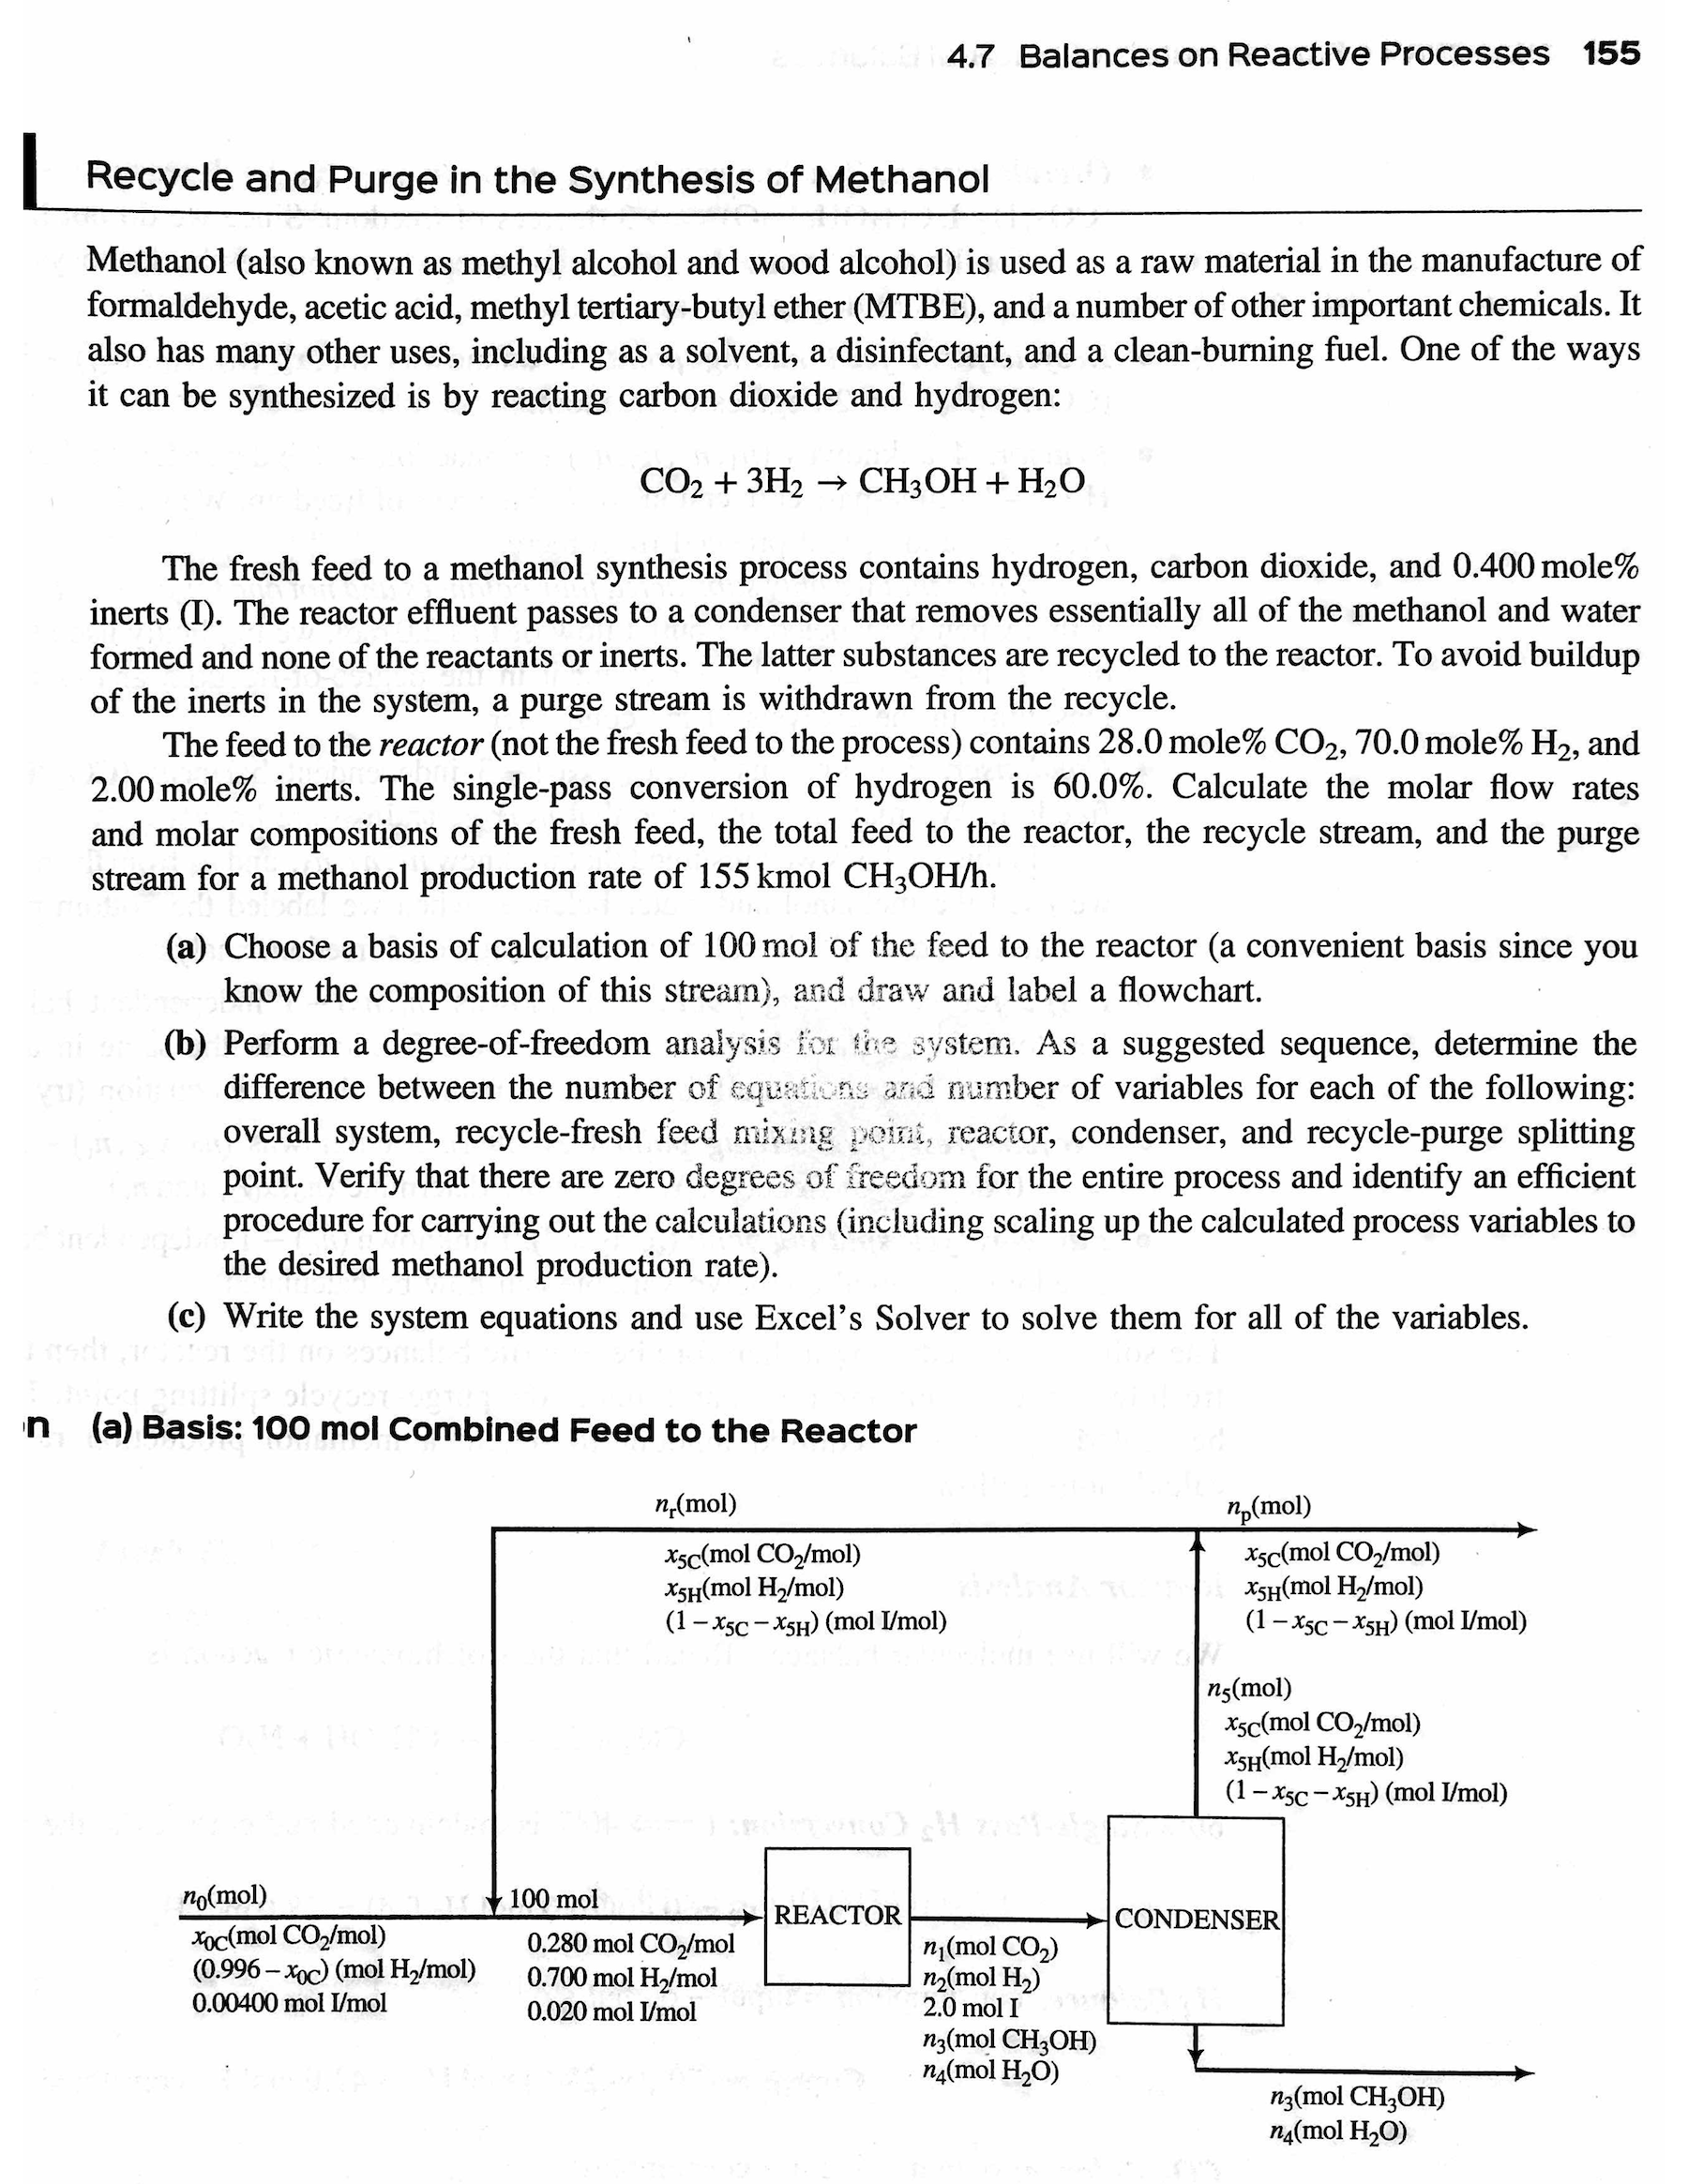
\includegraphics[width=.9\linewidth]{./figs/Purge.png}
\begin{itemize}
\item Reactor balance, 4 DOFs - 3 balances - 1 conversion:
\end{itemize}

\begin{center}
\begin{tabular}{rrrr}
\hline
\ce{CO2} & \ce{H2} & \ce{CH3OH} & \ce{H2O}\\
14.0 & 28.0 & 14.0 & 14.0\\
\hline
\end{tabular}
\end{center}

\begin{itemize}
\item Condenser balance, simple split, BUT, inert concentration goes up!!!!
\end{itemize}
\begin{center}
\begin{tabular}{rrr}
\hline
\ce{CO2} & \ce{H2} & Inert\\
14.0 & 28.0 & 2\\
\hline
\end{tabular}
\end{center}

\begin{itemize}
\item mixing point, non-reactive, 4 DOFs - 3 balances - 1 total
\end{itemize}

\begin{center}
\begin{tabular}{rr}
\hline
n\(_0\) & n\(_r\)\\
61.4 & 38.6\\
\hline
\end{tabular}
\end{center}

\begin{itemize}
\item purge split \(n_{5} = n_{r} + n_{p}\)
\end{itemize}

\begin{center}
\begin{tabular}{r}
\hline
n\(_p\)\\
5.4\\
\hline
\end{tabular}
\end{center}

\subsection{Combustion in air}
\label{sec-6-8}
\newpage

\section{Properties of single-phase systems}
\label{sec-7}
\begin{itemize}
\item Can't design a reactor around masses and moles; have to know sizes, volumes
\item \(\rho = \rho(T,P,x_{i}) \), example of what is called an equation of state
\item Material balances often require we know the physical properties (e.g, densities, thermal expansion coefficient, \ldots{}) of pure substance and of mixtures
\item Where to get this information?
\begin{itemize}
\item Look it up (Perry's handbook, literature)
\item Measure it (laboratory)
\item Estimate from physical property models
\item Compute from molecular models
\end{itemize}
\end{itemize}

\subsection{Liquid and solid densities}
\label{sec-7-1}
\begin{itemize}
\item Liquids and solids generally incompressible and small coefficients of thermal expansion
\item Pure densities from measurement or estimate
\item Mixture densities depend\ldots{}
\item Ideal solution (MeOH and \ce{H2O}) has additive molar volumes:
\end{itemize}
\[ v \text{ (l/mol)} = \sum_{i} x_{i} v_{i} \]
\begin{itemize}
\item or equivalently additive inverse densities (\(\omega_{i}\) are mass fractions):
\end{itemize}
\[ \frac{1}{\bar{\rho}} = \sum_{i}^{n} \frac{\omega_{i}}{\rho_{i}} \]
\begin{itemize}
\item Many solutions \textbf{not} ideal, e.g., ethanol/methyl formate positive deviation; methanol/methyl formate negative deviation
\item Sometimes other empirical relations are observed
\end{itemize}
\[ \bar{\rho} = \sum_{i}^{n} x_{i}\rho_{i}\]
\begin{itemize}
\item See \href{http://library.nd.edu/engineering/}{Perry's Handbook} for data
\end{itemize}

\subsection{Ideal gas}
\label{sec-7-2}

es
\begin{itemize}
\item Gas volumes are much more sensitive to temperature and pressure
\item Relationship captured in an ``equation of state''
\item Ideal gas equation of state very familiar
\end{itemize}

\[ P V = n R T \text{ or } P v = R T \text{ or } v = \frac{RT}{P} \]

\begin{itemize}
\item \emph{R} = gas constant is a fundamental physical constant of nature, closely related to concept of temperature
\end{itemize}

\begin{center}
\begin{tabular}{llll}
R & 8.314472 J / (K mol) & 0.082057 atm l / (K mol) & 1.3806504e-23 J / K\\
\end{tabular}
\end{center}
\begin{itemize}
\item \(v\) replaced by \(\dot{v}\) in flow context
\end{itemize}

\begin{quote}
\hline
\textbf{Ideal gas Flow} Butane at \SI{360}{\celsius} and 3.0 atm absolute pressure flows into a reactor at \SI{1100}{\kilogram\per\hour}.  Volumetric flow rate?
\hline
\end{quote}
\begin{minted}[frame=lines,fontsize=\scriptsize,linenos]{python}
R = 0.082057 # l atm/mol K
MW = (4*12.00 + 10 * 1.008)/1000 # kg/mol

T = 360 + 273.15 # K
P = 3.00 # atm
mdot = 1100 # kg/hr

vdot = (mdot/MW) * (R * T / P)
print('{0:6.2f} l/hr'.format(vdot))
\end{minted}

\begin{verbatim}
327994.88 l/hr
\end{verbatim}


\begin{quote}
\hline
\textbf{Ideal gas ratios} \SI{10}{ft\cubed} of air at 70 F and 1.00 atm is heated to 610 F and compressed to 2.50 atm.  Final volume?
\hline
\end{quote}
\begin{minted}[frame=lines,fontsize=\scriptsize,linenos]{python}
V0 = 10.
T0 = 70 + 459.67 # R
T = 610 + 459.67
P0 = 1. # atm
P = 2.50 # atm

V = V0*(P0/P)*(T/T0)
print('{0:6.2f} ft3'.format(V))
\end{minted}

\begin{verbatim}
8.08 ft3
\end{verbatim}

\begin{itemize}
\item \(v\) is only a function of $T$ and $P$, suggests ``standard'' volume at ``standard'' conditions, typically 273 K and 1 atm for SI/cgs, 32 F and 1 atm for English.
\end{itemize}

\[ v_{s} = 22.415~\text{L/mol} = 0.022415~\text{m}^{3}\text{/mol} = 359.05 \text{ ft}^{3}\text{/lb-mol}\]

\begin{quote}
\hline
\textbf{Standard gas} The flow rate of methane at 285 F and 1.30 atm absolute is reported to be \(3.95\times 10^5\) SCFH.  Molar flow rate?  Volumetric flow rate?
\hline
\end{quote}
\begin{minted}[frame=lines,fontsize=\scriptsize,linenos]{python}
VSCFH = 3.95e5 # std ft3/hr
PS = 1.0 #
P = 1.30 #
TS = 459.67 + 32 # R
T = TS + 285.

Vs = 359.05 # std ft3/lb-mol

ndot = VSCFH /Vs  # lb-mol/hr

V = VSCFH * ( PS/P) * (T/TS)

print('{0:6.2e} mol/hr   {1:6.2e} ft^3/hr'.format(ndot,V))
\end{minted}

\begin{verbatim}
1.10e+03 mol/hr   4.80e+05 ft^3/hr
\end{verbatim}

\subsection{Ideal gas mixture}
\label{sec-7-3}
\begin{itemize}
\item ideal mixture $\to$ volumes are additive:
\end{itemize}

\[ V(N,T,P) = V_{1}(N_{1},T,P) + V_{2}(N_{2},T,P) \]

\begin{itemize}
\item Called ``Amagat's Law,'' applies $\approx$ both ideal and non-ideal gases

\item individual components ideal gas $\to$ mixture is ideal gas:
\end{itemize}
\begin{eqnarray*}
V(N,T,P) & =  & \frac{N_{1} R T}{P} + \frac{N_{2} R T}{P} \\
         & =  & \frac{(N_{1}+ N_{2}) R T}{P} \\
         & =  & \frac{N R T}{P}
\end{eqnarray*}

\begin{itemize}
\item ``Partial pressures'' additive:
\end{itemize}
\begin{eqnarray*}
 P & = & \frac{N_{1} R T}{V} + \frac{N_{2} R T}{V}\\
   & = & P_{1} + P_{2}
\end{eqnarray*}

\begin{itemize}
\item Partial pressure proportional to mole fraction:
\end{itemize}

\[ \frac{P_{1}}{P} = \frac{N_{1} RT/V}{N RT/V} = y_{1}\]

\begin{itemize}
\item Volume fraction proportional to mole fraction:
\end{itemize}

\[ \frac{V_{1}}{V} = \frac{N_{1}}{N} = y_{1} \]

\begin{itemize}
\item Use mole fraction and volume fraction and partial pressure interchangeably for ideal gas mixture
\end{itemize}

\begin{quote}
\hline
\textbf{Partial Pressures}  Acetone and nitrogen mixed in an evaporator and flowed through a compressor.  Liquid acetone enters system at a flow rate of \SI{400}{\liter\per\minute} and exits at a partial pressure (gauge) of 501 mm Hg at \SI{325}{\celsius}.  Total pressure of exit is 6.2 atm (gauge).  What is flow rate and composition of exit?  Atmospheric pressure is 763 mm Hg.
\hline
\end{quote}

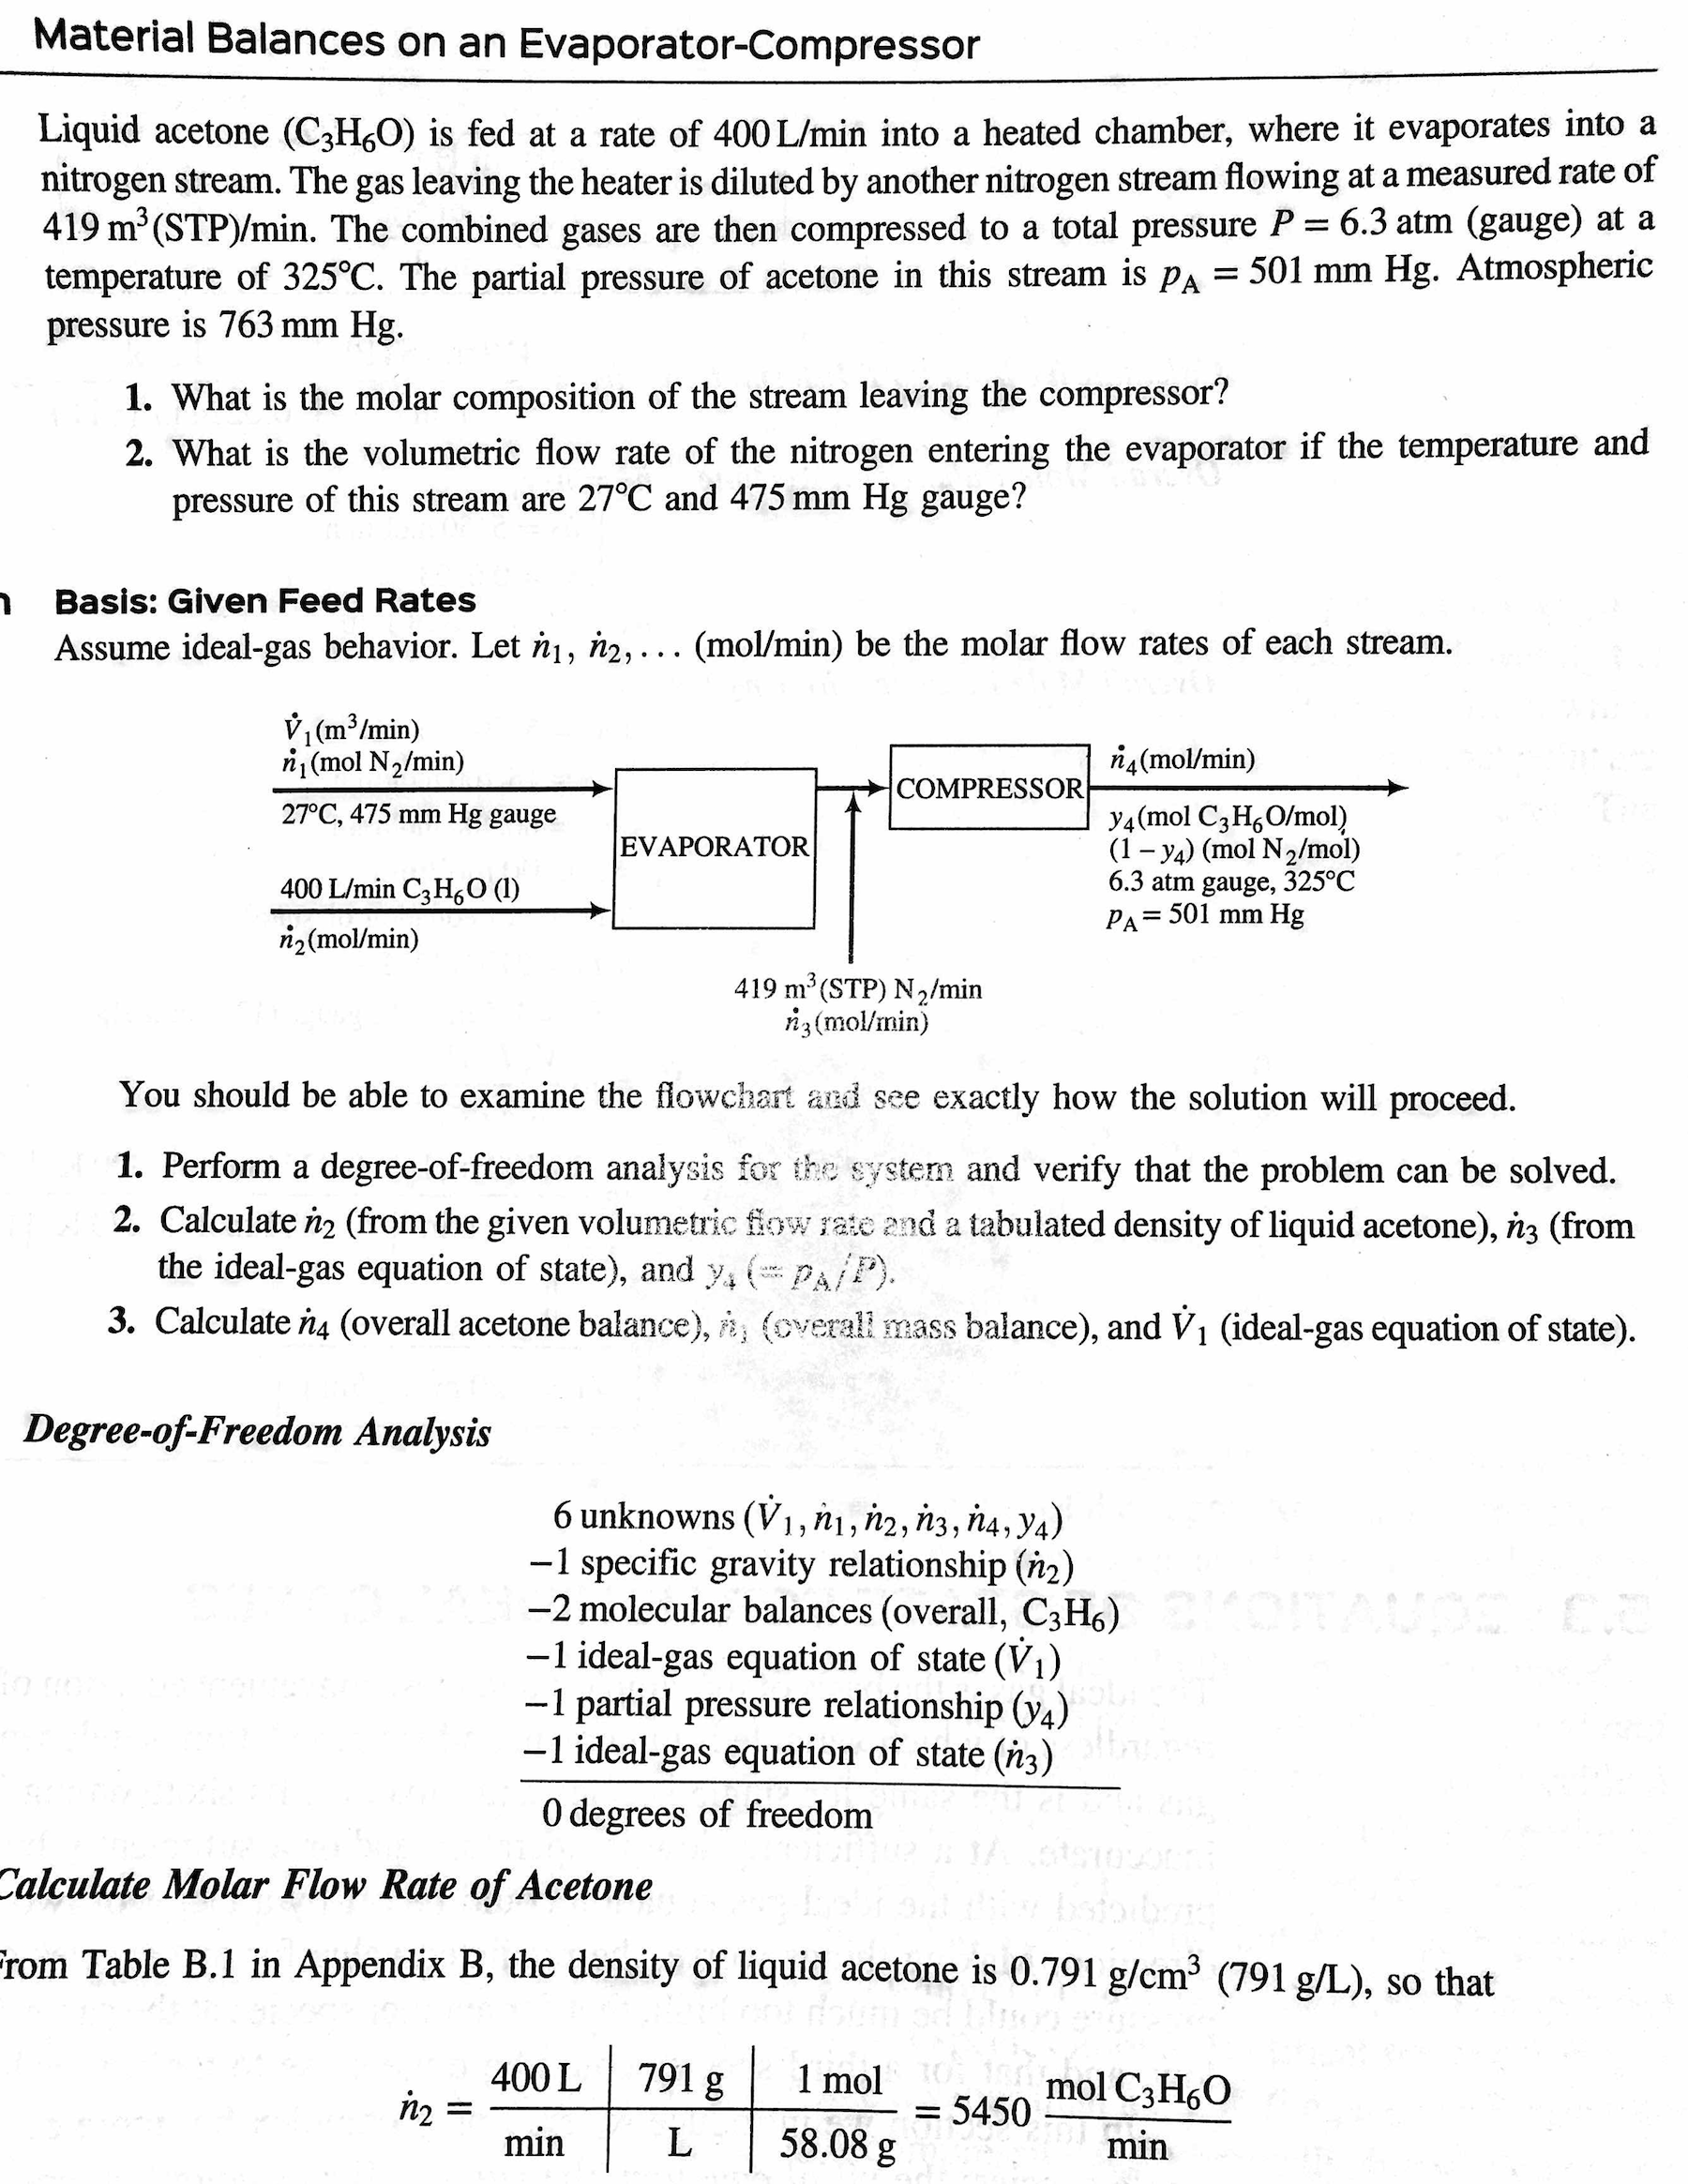
\includegraphics[width=0.95\textwidth]{./figs/PartialPressure.png}

\begin{minted}[frame=lines,fontsize=\scriptsize,linenos]{python}
rho_acetone = 0.791 # g/cm3
vdot_acetone = 400. # l/min
MW_acetone = 58.08 # g/mol

ndot_acetone = vdot_acetone * 1000. * rho_acetone / MW_acetone

print('acetone = {0:6.0f} mol/min'.format(ndot_acetone))

P_atm = 763.
P_exit = 6.2 * 760. + P_atm  # mm Hg
P_acetone = 501. + P_atm # mm Hg
P_N2 = P_exit - P_acetone
y_N2 = P_N2/P_exit; y_acetone = P_acetone/P_exit

print('acetone = {0:5.3f}  N2 = {1:5.3f} mol/mol'.format(y_acetone,y_N2))

n_exit = ndot_acetone * (1 + y_N2/y_acetone) # mol/min

T_exit = 325 + 273.15  # K

R = 62.36 # L mm Hg/mol K

V_exit = n_exit * R * T_exit /P_exit

print('exit {0:6.1f} mol/min  {1:6.1f} l/min'.format(n_exit,V_exit))
\end{minted}

\begin{verbatim}
acetone =   5448 mol/min
acetone = 0.231  N2 = 0.769 mol/mol
exit 23596.5 mol/min  160760.4 l/min
\end{verbatim}

\subsection{Real equations of state}
\label{sec-7-4}
\subsubsection{Ideal gas}
\label{sec-7-4-1}
\begin{itemize}
\item No condensation
\end{itemize}

\begin{minted}[frame=lines,fontsize=\scriptsize,linenos]{python}
import numpy as np
import matplotlib.pyplot as plt

import numpy as np
import matplotlib.pyplot as plt

R = 0.0821 # l atm/mol K
v = np.logspace(-0.2,1)

for T in np.arange(100.,1000,100):
    P = R * T *(1/v)
    plt.plot(v,P,label=T)

legend = plt.legend()

plt.xlabel('Volume (L/mol)')
plt.ylabel('Pressure (atm)')

plt.savefig('./figs/idealgas.png')
\end{minted}

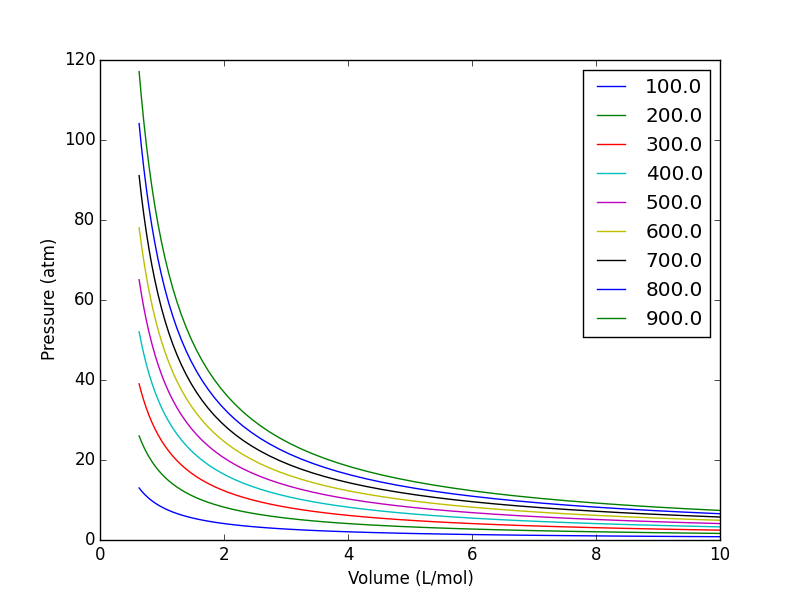
\includegraphics[width=.9\linewidth]{./figs/idealgas.png}

\subsubsection{van der Waals model}
\label{sec-7-4-2}
\begin{itemize}
\item molecules have volume: \(v\) $\to$ \(v - b\)
\item molecules attract: \(P\) $\to$ \( P - a/v^{2} \)
\end{itemize}

\[ P_{\text{vdW}} = \frac{RT}{v-b} - \frac{a}{v^{2}} \]

\begin{itemize}
\item ``cubic'' equation of state:
\end{itemize}
\[ v^{3} - \left (b + \frac{RT}{P}\right ) v^{2}+\frac{a}{P}v - \frac{ab}{P} \]

\begin{itemize}
\item \emph{b} has units of volume/mole

\item \emph{a} has units of pressure * (volume/mol)\(^{2}\) = energy * volume/mol
\end{itemize}

\begin{center}
\begin{tabular}{lrr}
\hline
 & a ((L/mol)2 bar & b (L/mol)\\
\hline
\ce{H2} & 0.2476 & 0.02661\\
\ce{N2} & 1.370 & 0.0387\\
\ce{CH4} & 2.283 & 0.04278\\
\ce{CO2} & 3.640 & 0.04267\\
\hline
\end{tabular}
\end{center}

\begin{minted}[frame=lines,fontsize=\scriptsize,linenos]{python}
import numpy as np
import matplotlib.pyplot as plt

R = 0.0821 # l atm/mol K

a = 3.640; b = 0.04267;

vc = 3 * b; Tc = (8./9.)*a /(R * vc); Pc = (R * Tc)/(vc-b) - a/(vc*vc);

vr = np.logspace(-0.5,1.)

plt.figure(1)
for Tr in np.arange(0.87,1.3,0.13):
    Pr = 8 * Tr/(3 * vr -1) - 3 *(1/vr) *(1/vr)
    plt.plot(vr*vc,Pr*Pc,label=Tr*Tc)

plt.title('CO2 van der Waals isotherms')
plt.ylim([.1*Pc,4*Pc])
plt.xlim([.3*vc,6*vc])
plt.xlabel('Volume (l/mol)')
plt.ylabel('Pressure (atm)')
legend=plt.legend()

plt.savefig('./figs/vdWgas.png')

plt.figure(2)
for Tr in np.arange(0.87,1.3,0.13):
    Pr = 8 * Tr/(3 * vr -1) - 3 *(1/vr) *(1/vr)
    plt.loglog(vr*vc,Pr*Pc,label=Tr*Tc,basex=10)

legend = plt.legend()

plt.ylim([.1*Pc,100*Pc])
plt.xlim([.3*vc,10*vc])
plt.xlabel('Log volume (l/mol)')
plt.ylabel('Log pressure (atm)')
plt.title('CO2 van der Waals isotherms')

plt.savefig('./figs/logvdWgas.png')
\end{minted}

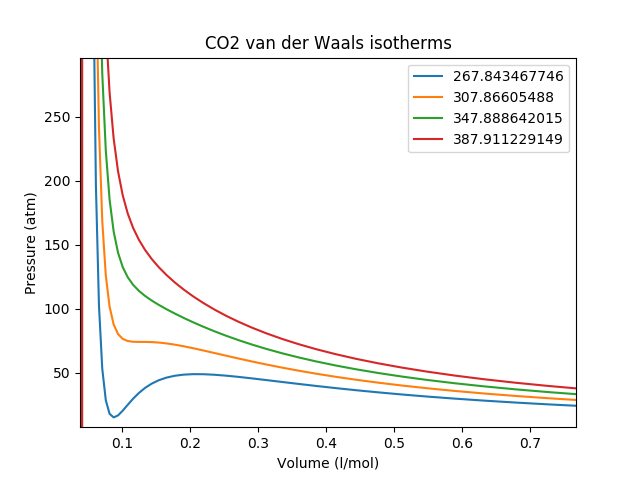
\includegraphics[width=.9\linewidth]{./figs/vdWgas.png}

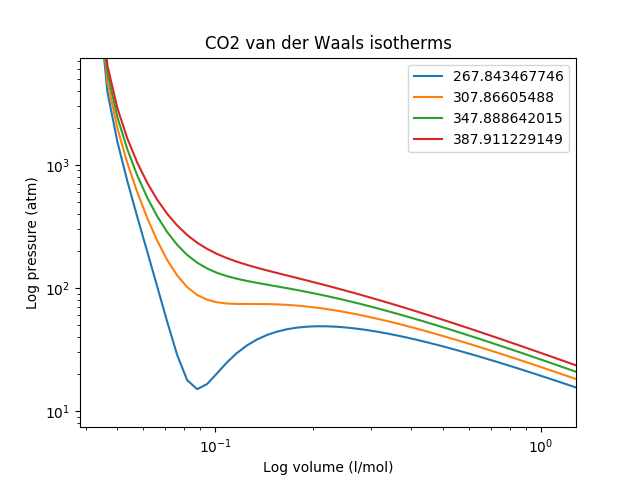
\includegraphics[width=.9\linewidth]{./figs/logvdWgas.png}

\begin{itemize}
\item At higher temperature, pressure and volume vary approximately inversely (gas)
\item At lower temperature, follow isotherm, reach region where compressing causes $P$ to go \emph{down}, unphysical,
\begin{itemize}
\item form two phases, dense (liquid) and dilute (vapor)
\item middle intersection point unphysical
\item One pressure and temperature at which two phases coexist (same chemical potential)
\item Called ``saturation pressure,'' \(P_{sat}(T)\)
\item Given volumes, easy to solve for \(P_{sat}\), other way not so easy (\(\mu_{v} = \mu_{l}\))
\end{itemize}

\item Transition point between the two regions, called the ``critical point''
\item \(T > T_{c}\), \(P>P_{c}\) called ``supercritical''
\item At critical point, density of liquid and vapor are the same
\item As move below the critical point, the densities/volumes move apart

\item Critical constants related to \emph{a} and \emph{b}:
\end{itemize}

\[b = v_{c}/3\quad\quad a = \frac{9}{8}R T_{c} v_{c}\]

\begin{itemize}
\item common to refer to the ``reduced'' temperature, pressure, volume, unitless, scaled to the critical values.  As we see below, many species behave the same in reduced variables
\end{itemize}

\[ T_{r} = T/T_{c}\quad P_{r} = P/P_{c}\quad v_{r}=v/v_{c}\]

\subsubsection{Other cubic equations of state}
\label{sec-7-4-3}
\begin{itemize}
\item vdW model qualitatively and theoretically important, practically not so accurate
\item more elaborate equations necessary to model real fluids more reliably
\item \emph{all} are approximations to reality
\item Soave-Redlich-Kwong (SRK) one common example (Peng-Robinson another)
\end{itemize}

\[P_{\text{SRK}} = \frac{RT}{v-b} - \frac{\alpha(T) a}{v(v+b)} \]

\begin{itemize}
\item still cubic in \emph{v}, so same qualitative form, but more parameters to fit
\end{itemize}

\begin{eqnarray*}
a & = & 0.42747 \frac{(R T_{c})^{2}}{P_{c}} \\
b & = & 0.08664 \frac{R T_{c}}{P_{c}} \\
m & = & 0.48508 + 1.55171 \omega - 0.1561 \omega^{2}\\
\alpha & = & \[1+m (1-\sqrt{T_{r}})\]^2
\end{eqnarray*}

\begin{itemize}
\item $\omega$ is so-called Pitzer ``acentric'' factor, compiled along with critical constants
\end{itemize}

\[\omega = -\log \left ( \frac{P_{sat}}{P_{c}} \right ) \Big|_{T_{r}=0.7} -1 \]

\begin{center}
\begin{tabular}{lrrr}
\hline
 & Pitzer factor & Tc (K) & Pc (atm)\\
\hline
\ce{N2} & 0.037 & 126.20 & 33.5\\
\ce{CH4} & 0.011 & 190.7 & 45.8\\
\ce{CO2} & 0.225 & 304.2 & 72.9\\
\hline
\end{tabular}
\end{center}

\begin{minted}[frame=lines,fontsize=\scriptsize,linenos]{python}
import numpy as np
import matplotlib.pyplot as plt

Tc =304.2; Pc = 72.9; omega = 0.225;
R = 0.0821 # l atm/mol K

a = 0.42747 * (R * Tc)**2 / Pc

b = 0.08664 * (R * Tc) /Pc

m = 0.48508 + (1.55171 - 0.1561 * omega )* omega

v = np.logspace(-1.5,0.)

plt.figure(1)
for T in np.arange(268,390,40):
    alpha = 1 + m * (1 - (T / Tc)**0.5)
    Psrk = R * T /(v-b) - alpha * a / (v* (v+b))
    Pig = R * T /v
    plt.plot(v,Psrk,label=T)
    plt.plot(v,Pig,label=T,ls='--')

plt.title('CO2 SRK isotherms')
plt.ylim([0,300])
plt.xlim([0.02,0.8])
plt.xlabel('Volume (l/mol)')
plt.ylabel('Pressure (atm)')
legend=plt.legend()

plt.savefig('./figs/SRKgas.png')

# plt.figure(2)
# for T in np.arange(268,390,40):
#     alpha = 1 + m * (1 - (T / Tc)**0.5)
#     Psrk = R * T /(v-b) - alpha * a / (v* (v+b))
#     plt.loglog(v,Psrk,label=T,basex=10)

# legend = plt.legend()

# plt.ylim([1e1,1e4])
# plt.xlim([0.01,1.1])
# plt.xlabel('Log volume (l/mol)')
# plt.ylabel('Log pressure (atm)')
# plt.title('CO2 SRK vs. Ideal Gas isotherms')

# plt.savefig('./figs/logSRKgas.png')
\end{minted}

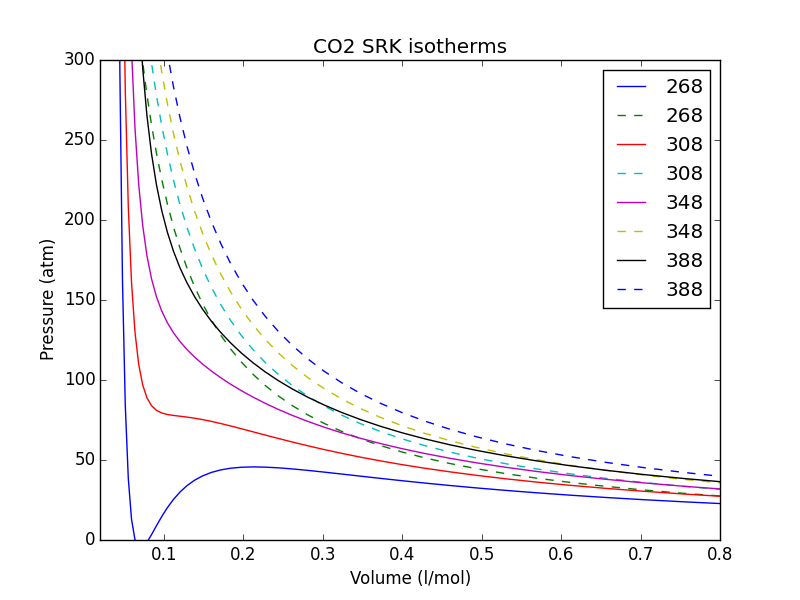
\includegraphics[width=.9\linewidth]{./figs/SRKgas.png}


\begin{itemize}
\item errors largest at low \emph{v}, low \emph{T}
\item given \emph{T} and \emph{v}, easy to find \emph{P}
\item given \emph{T} and \emph{P}, harder to find \emph{v}; solve numerically
\end{itemize}

\subsubsection{Virial expansion}
\label{sec-7-4-4}

\[ P= \frac{RT}{v} \left ( 1 + \frac{B_{2}(T)}{v} + \frac{B_{3}(T)}{v^{2}} + \cdots \right ) \]
\subsubsection{Law of corresponding states}
\label{sec-7-4-5}
\begin{itemize}
\item Observed empirically that \(PvT\) properties of many fluids behave similarly when expressed in terms of reduced variables
\item Reflects common competition between size/entropy and interaction/energy
\item Define unitless \emph{compressibility}:
\end{itemize}
\[ Z = \frac{P(v,T) v}{RT} \]

\begin{itemize}
\item \(Z_{ig} = 1 \)
\item \( Z_{c} = 0.27 \) for many common fluids
\item Plot of \emph{Z} vs. \(P_{r}\) for various \(T_{r}\)
\begin{itemize}
\item Negative deviations at low \emph{P}, attractions reduce pressure relative to ideal gas
\item Positive deviations at high \emph{P}, repulsive regime due to short-range repulsion
\item Deviations increase with decreasing \(T_{r}\)
\end{itemize}
\end{itemize}

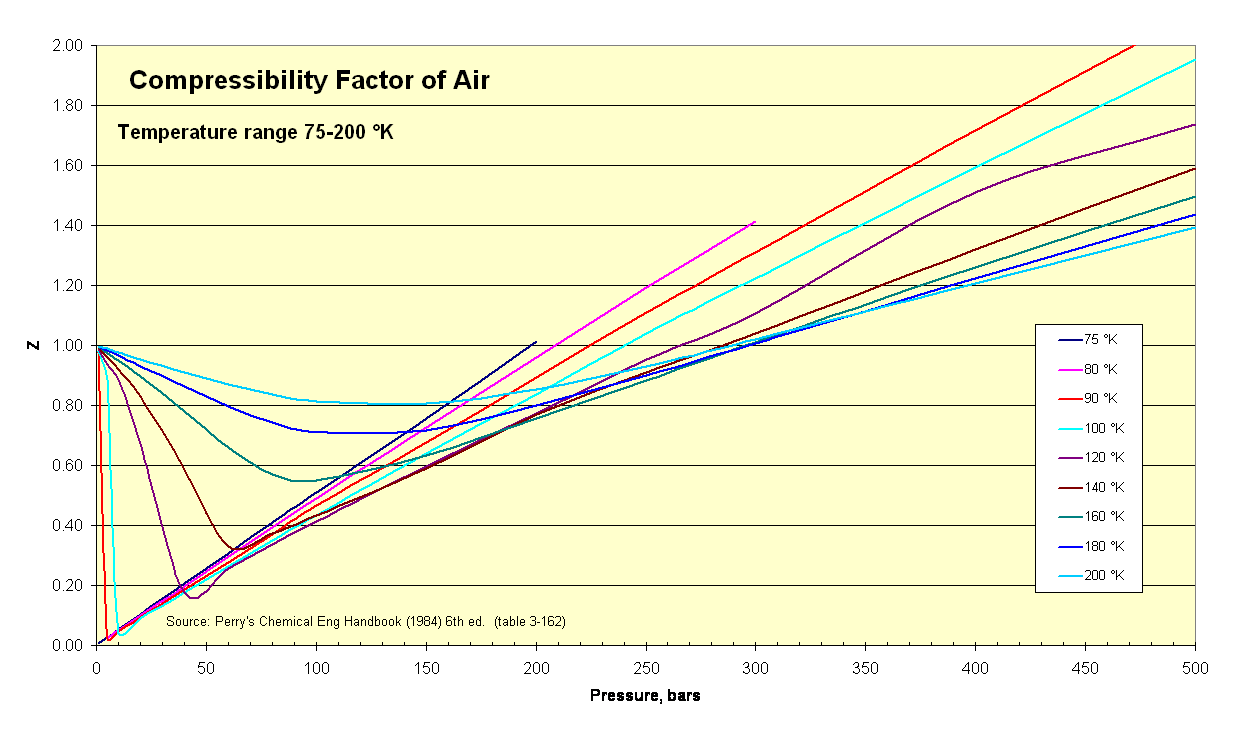
\includegraphics[width=.9\linewidth]{./figs/AirCompressibility.png}

\begin{itemize}
\item Algorithm: given two of \(PvT\) and corresponding critical constants, convert to reduced values, read unknown value off of compressibility chart, and back-convert to real value.
\item Rather arcane, not-computer-friendly way of getting \emph{PvT} information
\end{itemize}

\subsection{Real gas mixtures}
\label{sec-7-5}
\begin{itemize}
\item Even messier problem
\item Mixing rules to combine parameters from individual components
\end{itemize}
\newpage

\section{Two-phase systems}
\label{sec-8}
Very often interested in systems in which two distinct phases are present, e.g. \emph{l}-/g/.  Common in separations problems, including my favorite, extracting tasty coffee from coffee beans, and second favorite, \ce{CO2} from flue gas.

\subsection{One-component phase diagrams}
\label{sec-8-1}
\begin{itemize}
\item Pure substances can exist in multiple ``phases.''  \emph{s}, \emph{l}, \emph{v} familiar, but can have e.g. multiple solid phases, example C
\item Stable phase at any given condition is a function of \emph{T} and \emph{P}
\item Captured in a ``phase diagram,'' which shows which phase is stable at a give condition
\item Have already talked about properties of single phases
\item Often interested in \emph{phase transitions}, boundaries between two phases
\item Give example from vdW isotherm; for given \emph{T}, only one \emph{P} at which both phases
\item Mention heat flow
\item In two-phase region, temperature sets one and only one saturation pressure
\item Mention \emph{latent heat}
\item Change the temperature, change the saturation pressure

\item \ce{CO2} phase diagram representative:
\end{itemize}

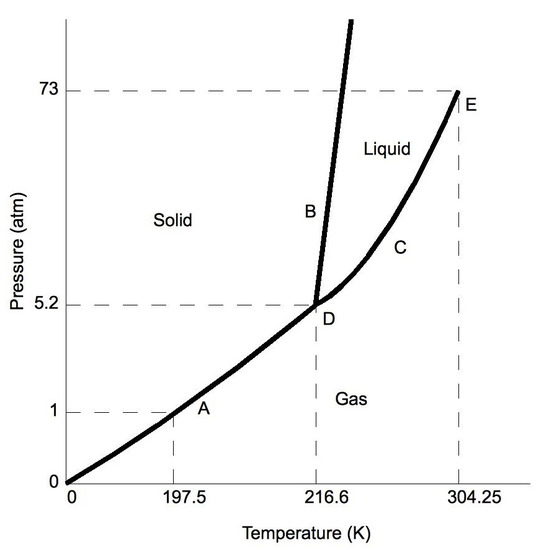
\includegraphics[width=0.8\textwidth]{./figs/CO2-Phase-Diagram.jpg}

\begin{itemize}
\item Key features:
\begin{itemize}
\item boiling point
\item ``normal'' boiling point
\item critical point and supercritical region
\item melting/freezing point
\item sublimation point
\item ``triple'' point
\end{itemize}

\item \ce{H2O} diagram somewhat anomalous:
\end{itemize}

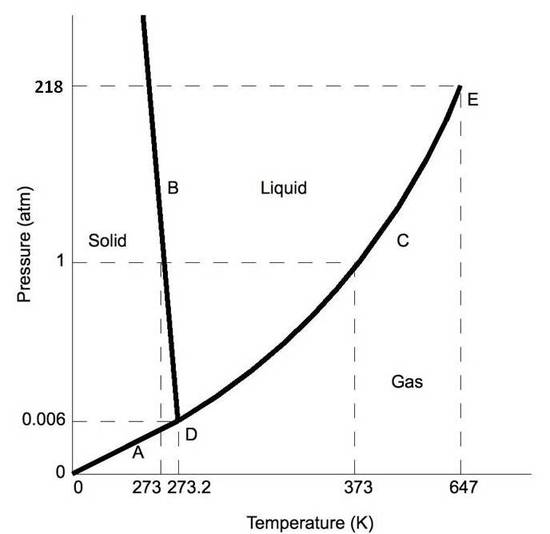
\includegraphics[width=0.8\textwidth]{./figs/H2O-Phase-Diagram.jpg}

\begin{itemize}
\item Will find tabulations of boiling/freezing points, critical points, triple points in Perry's Handbook, CRC, \url{http://webbook.nist.gov}
\end{itemize}

\subsubsection{Clapeyron equation}
\label{sec-8-1-1}
\begin{itemize}
\item Thermodynamics gives us a relationship for the slope of a coexistence line:
\end{itemize}
\[ \frac{d P^{*}}{dT} = \frac{\Delta H_{\text{latent}}}{T(v_{b}-v_{a})} \]

\begin{itemize}
\item Applied to liquid $\to$ vapor transition, ignoring liquid volume, and treating vapor as ideal gives the Clausius-Clapeyron equation:
\end{itemize}

\begin{eqnarray*}
\frac{d P^{*}}{dT} & = & \frac{\Delta H_{\text{vap}}}{T(v_{g}-v_{l})} \\
           & \approx & \frac{\Delta H_{\text{vap}}}{T v_{g}} \\
          & \approx & \frac{P \Delta H_{\text{vap}}}{R T^{2}} \\
\frac{d \ln P}{d 1/T} = - \frac{\Delta H_{\text{vap}}}{R}
\end{eqnarray*}

\begin{itemize}
\item Assuming \(\Delta H_{\text{vap}}\) is not a function of \emph{T}, integrates to
\end{itemize}

\[ \ln \frac{P^{*}_{2}}{P^{*}_{1}} = -\frac{\Delta H_{\text{vap}}}{R}\left ( \frac{1}{T_{2}} - \frac{1}{T_{1}} \right ) \]

\begin{itemize}
\item Plot of \(\ln P\) vs. \(1/T\) is approximately linear with slope related to latent enthalpy
\end{itemize}

\begin{quote}
\textbf{Clausius-Clapeyron example} Benzene normal boiling point is 353.2 K at 760 Torr.  Heat of vaporization is \SI{30.8}{\kilo\joule\per\mole}.  What is saturation pressure at 373.2 K?
\end{quote}

\begin{minted}[frame=lines,fontsize=\scriptsize,linenos]{python}
import numpy as np

R = 8.314
T1 = 353.2
T2 = 373.2
deltaH = 30800.

lnP = -(deltaH/R)*(1/T2 - 1/T1) + np.log(760)

P = np.exp(lnP)

print('ln P = {0:6.2f}  P = {1:6.0f} torr'.format(lnP,P))
print('Experiment = 1360 torr')
\end{minted}

\begin{verbatim}
ln P =   7.20  P =   1333 torr
Experiment = 1360 torr
\end{verbatim}

\subsubsection{Antoine equation}
\label{sec-8-1-2}
\begin{itemize}
\item Approximations underlying Clausius-Clapeyron are too severe for engineering work
\item Antoine equation is a modification empirically observed to fit saturation pressure/temperature data better:
\end{itemize}

\[ \log_{10}P^{*} = A - \frac{B}{T+C} \]

\begin{itemize}
\item Values of \emph{A}, \emph{B}, and \emph{C} are tabulated in standard references
\item Pay attention to units!
\item Because this is empirical, only apply within range of fit
\end{itemize}
\subsection{Gibbs phase rule}
\label{sec-8-2}
\begin{itemize}
\item In single-phase region, can specify both \emph{T} and \emph{P}---2 DOFs
\item At phase-boundary, only \emph{T} or \emph{P} is independent---1 DOF
\item Reflects Gibbs phase rule:
\end{itemize}

\[ DOF = c - \Pi - r + 2\]

\begin{itemize}
\item DOF are number of \emph{intensive} variables that can be freely set and still satisfy the composition conditions
\item Applies more generally to mixtures, including ones in which chemical reactions can occur
\end{itemize}

\subsection{Single-component VLE}
\label{sec-8-3}
\begin{itemize}
\item Common situation to have a liquid A (e.g. \ce{H2O}) in equilibrium with a vapor mixture (e.g. moist air)
\item Important in humidification, dehumidification, drying, evaporation, \ldots
\item At equilibrium, vapor is said to be ``saturated''
\item DOF = 2 - 2 + 2 = 2; any two of \(T, P, y_{1}\)
\end{itemize}

\subsubsection{Raoult's Law}
\label{sec-8-3-1}
\begin{itemize}
\item Pretty reliable relationship between variables is that partial pressure of volatile component is equal to saturation pressure:
\end{itemize}

\[ P_{i} = y_{i}P = P_{i}^{*}(T) \]

\begin{quote}
\textbf{Raoult's Law Example}  Saturation pressure of \ce{H2O} is 289 mmHg at \SI{75}{\celsius} (See Appendix of book).  What is equilibrium composition of air at this temperature?  (This would correspond to 100\% relative humidity.  Wet!)
\end{quote}

\begin{minted}[frame=lines,fontsize=\scriptsize,linenos]{python}
psat = 289.
yH2O = psat/760.
yair = 1. - yH2O
yN2 = 0.79*yair
yO2 = 0.21*yair

print('H2O = {0:3.0f}%  N2 = {1:3.0f}%  O2 = {2:3.0f}%'.format(yH2O*100,yN2*100,yO2*100))
\end{minted}

\begin{verbatim}
H2O =  38%  N2 =  49%  O2 =  13%
\end{verbatim}

\begin{itemize}
\item Raoult's Law applies to equilibrium.  Change any constraint, other variables must adjust to restore equilibrium
\item Often two-phase systems are \textbf{not} at equilibrium
\item Uncommon for vapor composition to be greater than equilibrium---vapor would just condense
\item Opposite is possible, if there isn't enough liquid phase to saturate the vapor
\item A ``superheated'' vapor is one that is below its saturation pressure
\end{itemize}

\[ y_{i} P < P_{i}^{*}(T) \]

\begin{itemize}
\item Called superheated because vapor would have to be cooled at constant pressure and composition to reach equilibrium
\item Or compressed at constant \emph{T}; at least one of three variables has to change
\item (Lower) temperature at which a superheated vapor would start to condense at constant \emph{P} is called ``dew point temperature''
\end{itemize}

\[ y_{i} P = P_{i}^{*}(T_{\text{dewpt}}) \]

\begin{itemize}
\item \( T - T_{\text{dewpt}} =\) degrees of superheat
\end{itemize}

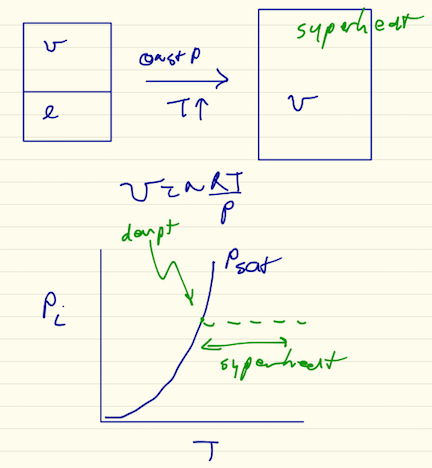
\includegraphics[width=.9\linewidth]{./figs/Superheat.png}

\begin{quote}
\textbf{Superheat example}  A stream of air is at \SI{100}{\celsius}, 5260 mmHg, and contains 10.0\% \ce{H2O}.  (1) Dewpoint?  (2) Degrees of superheat?  (3) Fraction of vapor that condenses and final gas phase composition if cooled to \SI{80}{\celsius} at constant \emph{P}?  (4) Ditto if air is isothermally compressed to 8500 mmHg.
\end{quote}

\begin{minted}[frame=lines,fontsize=\scriptsize,linenos]{python}
import scipy.optimize as opt

T0 = 100.        # C
P0 = 5260.       # mmHg
yH2O0 = 0.10
Psat = 760.      # duh!  Psat = Patm at 100 C!  We all know that.

PH2O = P0 * yH2O0

print('Partial pressure of H2O = {0:4.0f} mmHg'.format(PH2O))

dewpoint = 90.0   # from table
superheat = T0 - dewpoint
print('Dew point = {0:4.0f} degC    Superheat = {1:4.0f} degC'.format(dewpoint,superheat))

# Cool isobarically to 80 C
Psat80 = 355.1  # mmHg
yH2O80 = 355.1/5250

# draw a condenser feed and do mass balance on both streams
n0H2O = 0.1*100; n0air = 0.9*100;

# air balance
ndotv = 100 * 0.9 / (1 - yH2O80)

# H2O balance

ndotH2O = 100* 0.1 - ndotv * yH2O80

deltaH2O = (ndotH2O)/n0H2O

print('80 C composition ={0:6.4f}'.format(yH2O80))

print('Fraction of water condensed ={0:3.0f}%\n'.format(deltaH2O*100))

# Compress isothermally to 8500 mmHg at 100 C
Pcomp = 8500
PH2O = yH2O0 * 8500

print('Partial pressure of H2O = {0:4.0f} mmHg'.format(PH2O))

yH2Ocomp = Psat/Pcomp

# air balance
ndotv = 100 * 0.9 / (1 - yH2Ocomp)

# H2O balance

ndotH2O = 100* 0.1 - ndotv * yH2Ocomp

deltaH2O = (ndotH2O)/n0H2O

print('8500 mmHg composition ={0:6.4f}'.format(yH2Ocomp))

print('Fraction of water condensed ={0:3.0f}%\n'.format(deltaH2O*100))
\end{minted}

\begin{verbatim}
Partial pressure of H2O =  526 mmHg
Dew point =   90 degC    Superheat =   10 degC
80 C composition =0.0676
Fraction of water condensed = 35%

Partial pressure of H2O =  850 mmHg
8500 mmHg composition =0.0894
Fraction of water condensed = 12%

\end{verbatim}

\begin{itemize}
\item If \(P^{*} < P\), liquid \emph{evaporates} from surface
\item If \(P^{*} \ge P\), liquid \emph{boils} throughout
\end{itemize}

\subsubsection{Humidity}
\label{sec-8-3-2}
\begin{itemize}
\item These concepts very often applied to \ce{H2O}, in which we refer to \ce{H2O} vapor as \emph{humidity}
\item Common to define \emph{relative humidity}, fraction of maximum \ce{H2O} in air at given \emph{T}
\end{itemize}

\[ RH(T) = P_{\ce{H2O}}/P^{*}_{\ce{H2O}}(T) \]

\begin{quote}
\hline
\textbf{Relative humidity example} Humid air at \SI{75}{\celsius}, 1.1 bar, and 30\% RH is fed into a process unit at \SI{1000}{\meters\cubed\per\hour}.  Determine molar flow rate of all components.
\hline
\end{quote}
\begin{minted}[frame=lines,fontsize=\scriptsize,linenos]{python}
Psat75 = 289.  # mmHg
RH = 0.30
P = 1.1 * 760 / 1.01325 # torr

PH2O = RH*Psat75

print('PH2O = {0} torr'.format(PH2O))

yH2O = PH2O/P
yN2  = (1-yH2O)*0.79
yO2  = (1-yH2O)*0.21

print('H2O = {0}  N2 = {1}  O2 = {2} mol/mol'.format(yH2O,yN2,yO2))

# MWavg = (18. * yH2O + 28 * yN2 + 32 * yO2)/1000.   # kg/mol

R = 8.314
T = 75 + 273
P = 1.1e5         # Pa
vdot = 1000.      # m3/hr
ndot = P * vdot / ( R * T)

print('H2O = {0}  N2 = {1}  O2 = {2} mol/hr'.format(yH2O*ndot,yN2*ndot,yO2*ndot))
\end{minted}

\begin{verbatim}
PH2O = 86.7 torr
H2O = 0.10508226674641148  N2 = 0.7069850092703349  O2 = 0.18793272398325359 mol/mol
H2O = 3995.147826441919  N2 = 26879.03211994477  O2 = 7145.05917112456 mol/hr
\end{verbatim}

\subsection{Multi-component VLE}
\label{sec-8-4}

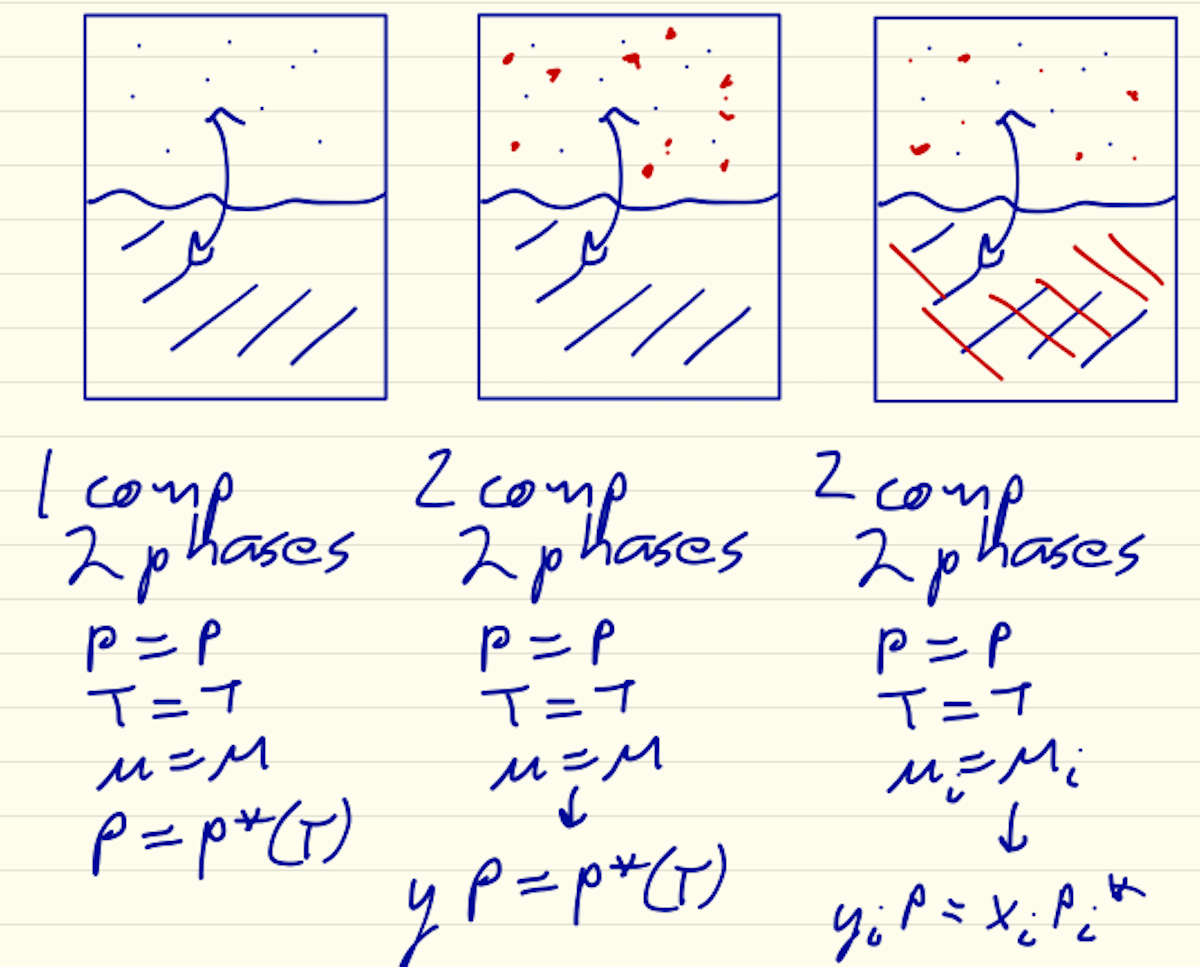
\includegraphics[width=0.8\textwidth]{./figs/VLE.png}

\begin{itemize}
\item Combine two liquids, both of which have finite (but different) Psat at given
\emph{T}, in a closed container
\item Vapor composition will in general be different from liquid.
\item Given a liquid composition (\emph{x}), ``bubble point'' is \emph{P} or \emph{T} at which first bit of vapor appears
\item Given a vapor composition (\emph{y}), ``dew point'' is \emph{P} or \emph{T} at which first bit of condensate appears
\end{itemize}

\subsubsection{Raoult's Law}
\label{sec-8-4-1}
\begin{itemize}
\item One model for VLE, most appropriate for majority material $\to$ 100\%
\item Partial pressure is saturation pressure scaled by fraction of molecules at surface:
\end{itemize}

\[ x_{A} P^{*}_{A}(T) = P_{A} = y_{A} P \]

\begin{itemize}
\item Assumes ideal liquid mixture and ideal gas mixture

\item If liquid only contains condensable components (\(\sum_{i} x_{i} = 1\))
\end{itemize}

\[ P_{\text{bubble}} = \sum x_{i} P_{i}^{*} \]

\begin{itemize}
\item Given \(x_{i}\), \emph{P}, can find \(y_{i}\):
\end{itemize}

\[ y_{i} = x_{i} P_{i}^{*} / P \]

\begin{itemize}
\item If we know the vapor composition \(y_{i}\), can determine the dew point by substitution from
\end{itemize}

\[ \sum_{i} x_{i} = 1  \to P_{\text{dew}} = \left ( \sum_{i}\frac{y_{i}}{P_{i}^{*}} \right )^{-1} \]

\begin{minted}[frame=lines,fontsize=\scriptsize,linenos]{python}
import numpy as np
import matplotlib.pyplot as plt

xB = np.linspace(0,1)
PAs = 10
PBs = 5

PB = xB * PBs
PA = (1-xB) * PAs
P = PA + PB

yB = PB/P

plt.plot(xB,P,yB,P)
# plt.plot(xB,PB,xB,PA,xB,P)
plt.ylabel('Pressure')
plt.xlabel('x_B, y_B')
plt.title('Isothermal compression')
plt.legend(['Bubble (x)','Dew (y)'])

plt.savefig('./figs/PressureVLE.png')
\end{minted}

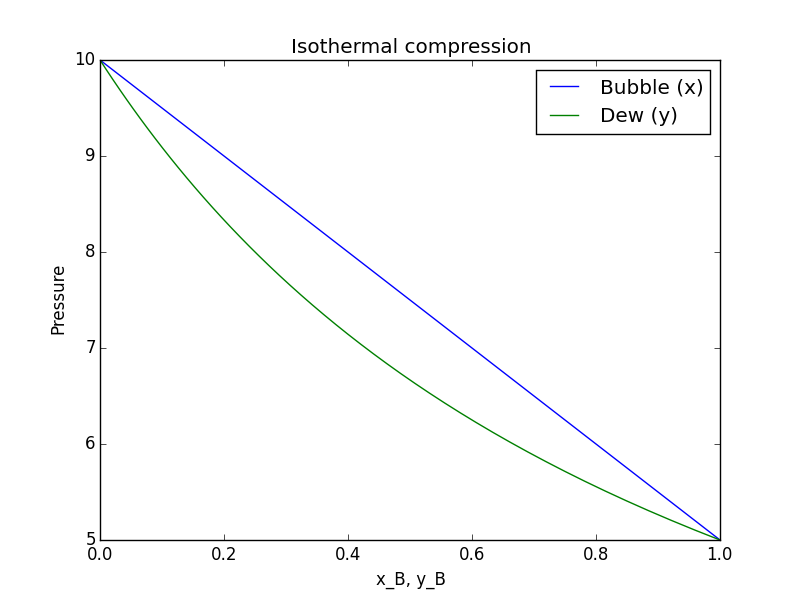
\includegraphics[width=.9\linewidth]{./figs/PressureVLE.png}

\begin{itemize}
\item Go up in pressure starting from 50:50 mix, hit dew line, first drop of liquid forms
\item Called dew pressure
\item Has composition of bubble line
\item Keep going up, vapor gradually condenses, composition follows dew line, liquid follows bubble line
\item Finally at bubble pressure last bit of vapor disappears
\item Call \emph{Px} diagram
\end{itemize}

\begin{quote}
\hline
\textbf{Bubble pressure example} 15\% benzene and 10\% toluene in \ce{N2} at \SI{80}{\celsius}.  At what pressure does vapor condense, and what is its composition?  Answer: condenses when partial pressure matches dew point.
\hline
\end{quote}
\begin{minted}[frame=lines,fontsize=\scriptsize,linenos]{python}
PBs = 756  # torr
PTs = 291  # torr
yB  = 0.15
yT  = 0.10

# eliminate xB
P = 1/((yB/PBs) + (yT/PTs))

xB = yB * P /PBs

print('Dew point pressure = {0:5.0f}  Benzene fraction = {1:5.3f}'.format(P,xB))
\end{minted}

\begin{verbatim}
Dew point pressure =  1845  Benzene fraction = 0.366
\end{verbatim}

\begin{itemize}
\item Can similarly create \emph{Tx} diagram at constant \emph{P}
\item Need model for how saturation pressure varies with \emph{T}
\end{itemize}

\begin{minted}[frame=lines,fontsize=\scriptsize,linenos]{python}
import numpy as np
import matplotlib.pyplot as plt
from scipy.optimize import fsolve

def PAs(T):
    A = 6.89272; B= 1203.531; C=219.888 # benzene Antoine
    logP = A - B/(T+C)
    return 10**logP
#    PA0 = 10
#    H = 800
#    return PA0 * np.exp(-H/T)

def PBs(T):
    A = 6.95805; B= 1346.773; C=219.693 # toluene Antoine
    logP = A - B/(T+C)
    return 10**logP

Pressure = 760.0

def PAsopt(T):
    return PAs(T) - Pressure

def PBsopt(T):
    return PBs(T) - Pressure

TA = fsolve(PAsopt,100)
TB = fsolve(PBsopt,100)

print(TA,TB)

T = np.linspace(TA,TB)

xB = (Pressure - PAs(T))/(PBs(T) - PAs(T))

yB = xB * PBs(T)/Pressure

plt.plot(xB,T,yB,T)
plt.xlim(0,1)
plt.ylabel('Temperature')
plt.xlabel('x_B, y_B')
plt.title('Isobaric heating')
plt.legend(['Bubble (x)','Dew (y)'])

plt.savefig('./figs/TemperatureVLE.png')


print(PAs(90)/760,PBs(90)/760)
\end{minted}

\begin{verbatim}
[ 80.10179978] [ 110.62216089]
1.343213901504202 0.5351810463458321
\end{verbatim}

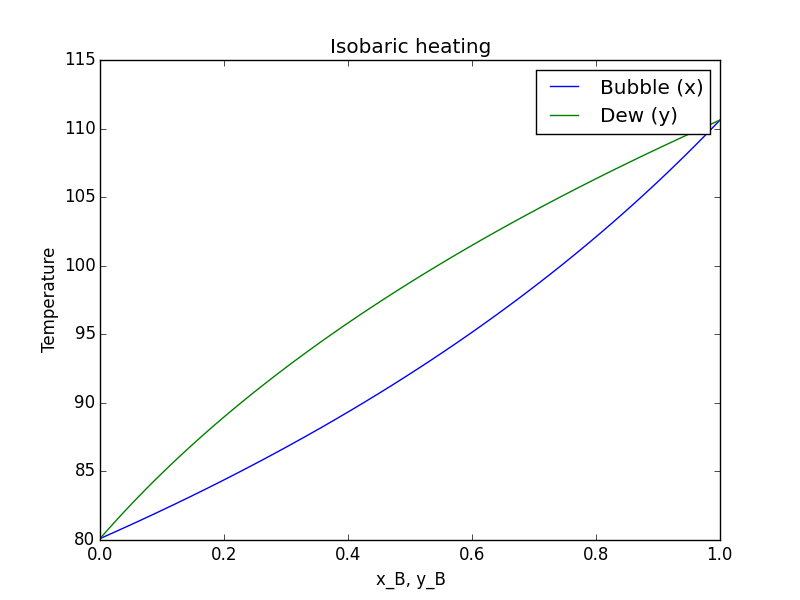
\includegraphics[width=.9\linewidth]{./figs/TemperatureVLE.png}

\subsubsection{Henry's Law}
\label{sec-8-4-2}
\begin{itemize}
\item Model appropriate for a dilute solute
\end{itemize}

\[ x_{A} H_{A}(T) = P_{A} = y_{A} P \]

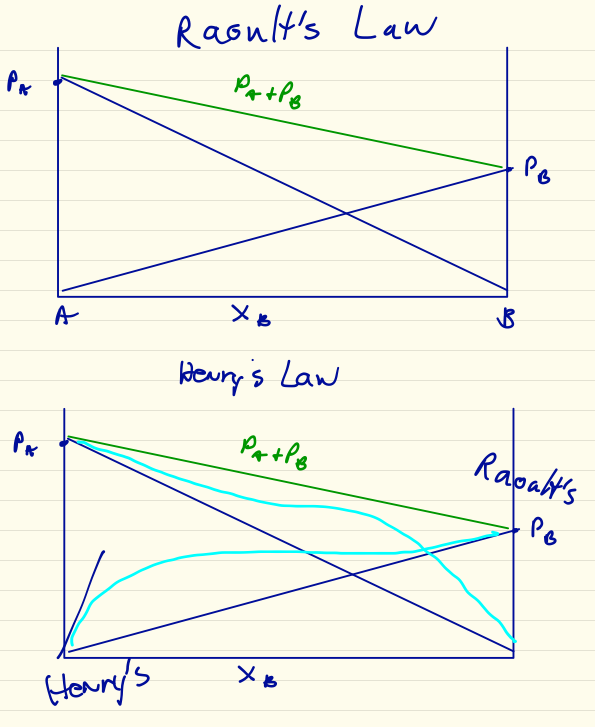
\includegraphics[width=0.8\textwidth]{./figs/Henry.png}

\begin{itemize}
\item Henry's constants are measured and tabulated
\end{itemize}

\subsubsection{Tabulations}
\label{sec-8-4-3}

\begin{quote}
\hline
\textbf{VLE example from tabulation} In this example, partial pressures of \ce{H2O} and \ce{SO2} over a solution of a given composition and temperature are read from a compilation.
\hline
\end{quote}

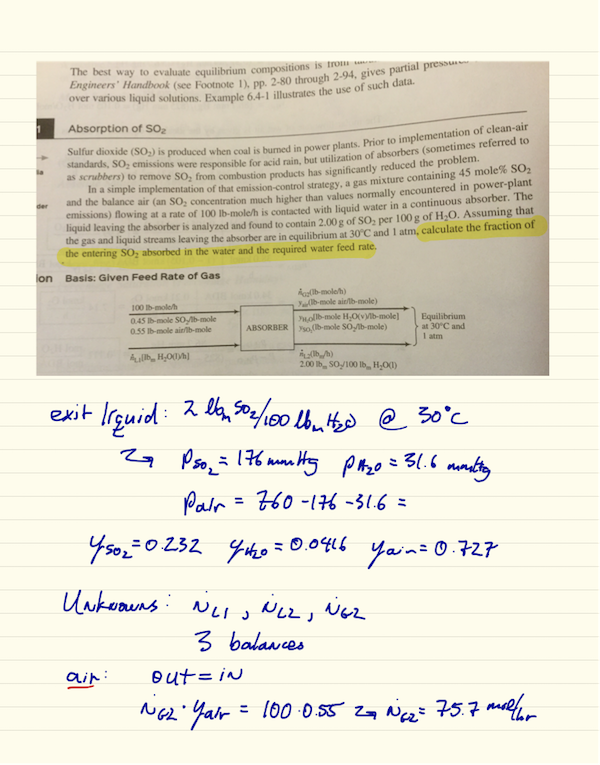
\includegraphics[width=1.0\textwidth]{./figs/VLE1.png}

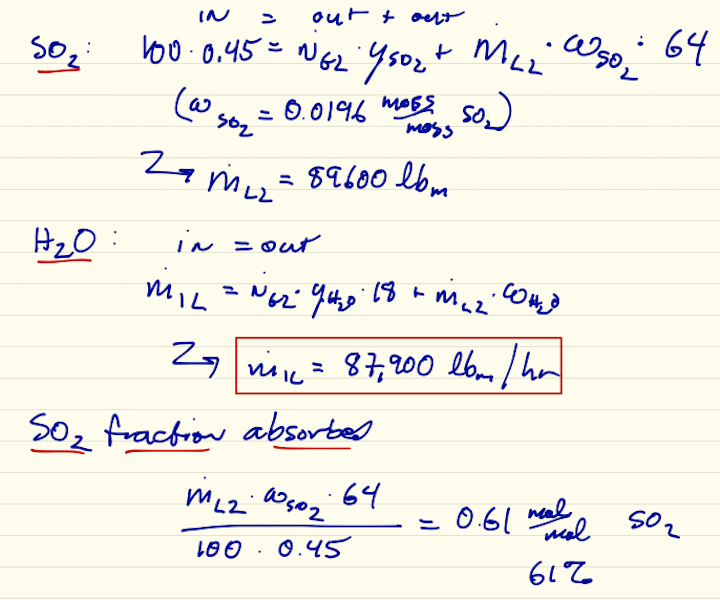
\includegraphics[width=1.0\textwidth]{./figs/VLE2.png}

\subsection{Solid-liquid}
\label{sec-8-5}
\subsubsection{Solubility}
\label{sec-8-5-1}
\begin{itemize}
\item Solids have limited solubility in liquids, called solubility limit.  Strong function of \emph{T} and of what exactly precipitates (anhydrous, hydrate, \ldots{})
\end{itemize}
\subsubsection{Colligative properties}
\label{sec-8-5-2}
\begin{itemize}
\item influence of solute on properties of solvent, depends on number but not type of solute
\item vapor pressure lowering $\to$ boiling point elevation
\item vapor pressure lowering $\to$ melting point lowering
\item combine Raoult's Law and Clausius-Clapeyron equation:
\end{itemize}

\[\Delta T_{b} = \frac{R T_{b}^{2}}{\Delta H^{*}_{vap}}x \]

\[\Delta T_{m} = \frac{R T_{m}^{2}}{\Delta H^{*}_{m}}x \]

\begin{itemize}
\item Can run in both directions, know composition, predict \emph{T} change, know \emph{T} change, compute \emph{x}
\end{itemize}

\begin{quote}
\hline
\textbf{EXAMPLE} 5.000 g solute in 100.0 g \ce{H2O} at 1 atm boils at \SI{100.421}{\celsius}.  Molecular weight of solute?
\hline
\end{quote}

\begin{minted}[frame=lines,fontsize=\scriptsize,linenos]{python}
R = 8.31441
Hb = 40656.   # J/mol
Tb = 273.16 + 100.   # K
dT = 100.421 - 100.

x = dT * Hb / (R * Tb * Tb ) # mol fraction solute

nH2O = 100.0 / 18.011   # mol

nSol = nH2O * x /(1-x)

MW = 5.000/nSol

print('Moles solute = {0:5.3f}   MW = {1:5.3f} g/mol'.format(nSol,MW))
\end{minted}

\begin{verbatim}
Moles solute = 0.083   MW = 60.014 g/mol
\end{verbatim}

\subsection{Liquid-liquid}
\label{sec-8-6}
\begin{itemize}
\item Two liquids that can be mixed in any proportions (ethanol and \ce{H2O}) are called \emph{miscible}
\item Two that do not mix (hexane and \ce{H2O}) are called \emph{immiscible}
\item Two that mix in only some proportions are called \emph{partially miscible}
\item Often expressed in terms of a \emph{partition coefficient} of a solute between two solvents
\item Or on a ternary phase diagram
\item Gibbs phase rule: dof = 3-2 + 2 = 3
\begin{itemize}
\item \emph{T}, \emph{P}, one composition variable fixes all the others
\end{itemize}
\item Basis of liquid-liquid extraction
\begin{itemize}
\item A = \ce{H2O}, B = acetone, C = MIBK
\end{itemize}
\end{itemize}

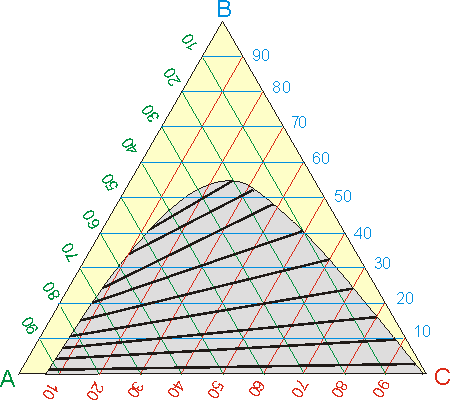
\includegraphics[width=0.6\textwidth]{./figs/Ternary.png}

\subsection{Solid-gas}
\label{sec-8-7}
\begin{itemize}
\item isotherms
\end{itemize}

\newpage
\section{Energy balances}
\label{sec-9}
\subsection{What's energy?}
\label{sec-9-1}
\begin{itemize}
\item kinetic (\(E_{K}\)), translational or rotational energy
\[ E_{K} = \frac{1}{2} m v^{2}\]
\item potential  (\(E_{V}\)), due to position with respect to an external field (gravitational, electric, magnetic)
\[ E_{grav} = m g h \]
\item internal energy (\(U\)), stored in bonds, in motion of molecules relative to one another, \ldots{}
\begin{itemize}
\item \emph{thermal} energy is one subset of internal
\item strong function of chemical composition, of phase, of \emph{T}, usually weak function of \emph{P}
\end{itemize}
\item energy is \emph{additive}, so \( E_{tot} = E_{K} + E_{V} + U \)
\item energy is \emph{conserved}, so for all processes, \(\Delta E_{\text{universe}} = 0\)
\begin{itemize}
\item First Law of Thermodynamics!
\end{itemize}
\end{itemize}

\subsection{Closed system (little different from thermo definition)}
\label{sec-9-2}
\begin{itemize}
\item distinguish \emph{system} from \emph{surroundings}
\item no \emph{material} crosses boundary
\item \emph{energy} can be transferred as heat (\emph{q}) - positive when added to a system
\item \emph{energy} can be transferred by doing work (\emph{w}) - positive when done on a system
\item basic balance for a closed system:
\end{itemize}

\[ \Delta E_{sys} + \Delta E_{sur} = 0\]

\[ \Delta U + \Delta E_{K} + \Delta E_{V} - q - w = 0 \]

\begin{itemize}
\item If system is not accelerating, \(\Delta E_{K} = 0 \)
\item If system is not rising or falling, \(\Delta E_{V} = 0 \)
\item \emph{adiabatic} process has \( q = 0 \)
\item If no mechanical interactions with surroundings (shaft, piston, magnetic rotor) \( w = 0 \)
\end{itemize}

\begin{framed}
\noindent \textbf{EXAMPLE} Gas in a cylinder.  (a) Add 2~kcal of heat and temperature rises from 25 to \SI{100}{\celsius} while piston is fixed.  (b) Piston is released, does 100 J of work, temperature of gas is constant.

(a) \(\Delta E_{K} = \Delta E_{V} = w = 0\).  \(q = 2 * 1000 * 4.184 = 8368~\text{J}\).  \(\Delta U = 8368~\text{J}\).

(b) \(\Delta E_{K} = \Delta E_{V} = 0\).  \(\Delta U = 0 \) if gas is ideal.  \(w = -100~\text{J} \) \to \(q = 100~\text{J} \).
\end{framed}

\subsection{Open system, steady state}
\label{sec-9-3}
\begin{itemize}
\item In open system at steady-state, energy balance changes to a power balance:
\end{itemize}

\[ \Delta\dot{U} + \Delta\dot{E}_{K} + \Delta \dot{E}_{V} - \dot{q} - \dot{w} = 0 \]

\begin{itemize}
\item Each delta is a sum over all the output less all the input streams.  Let's take these pieces apart.
\end{itemize}



\subsubsection{Flow and shaft work}
\label{sec-9-3-1}
When material flows through a system, work is done \emph{on} the system as material is pushed in and done \emph{by} the system as material is pushed back out.  Helpful to define some terms.

\begin{itemize}
\item \emph{shaft work} (\(\dot{W}_{s}\))is work done by a moving part on a system (like a turbine or rotor)
\item \emph{flow work} (\(\dot{W}_{f}\)) is difference between work done by fluid moving in and out of system
\end{itemize}

\[ \dot{W}_{f} = P_{\text{in}}\dot{V}_{\text{in}}-P_{\text{out}}\dot{V}_{\text{out}} \]

\begin{itemize}
\item If fluid is incompressible and there are frictional losses, what must be true about \( \dot{V}\)?  What is true about \( P_{in} - P_{out}\)?

\item Conventional to define a new thermodynamic function, \emph{enthalpy}, to include the flow work:
\end{itemize}

\[ H = U + PV \]

\begin{itemize}
\item energy balance becomes
\end{itemize}

\[ \Delta\dot{H} + \Delta\dot{E}_{K} + \Delta{E}_{P} = \dot{q} + \dot{W}_{s} \]

\subsubsection{Specific properties}
\label{sec-9-3-2}
\begin{itemize}
\item \emph{specific} property is (extensive) property per unit mass or per unit moles. Book uses both, so watch!

\item specific volume \(\hat{V} = 1/\rho \)  l/g

\item related to flow rate via mass flow rate
\end{itemize}
\[ \dot{V} = \dot{m}\hat{V} \]

\begin{itemize}
\item \emph{U} and \emph{H} are properties of the chemical species but not time, tabulated on a per mole or per mass basis
\item If on a per mole basis, related to molar flow rate
\end{itemize}
\[\dot{U} = \hat{U}\dot{n}\quad \dot{H} = \hat{H}\dot{n}  \]

\begin{framed}
\noindent \textbf{EXAMPLE} Specific internal energy and volume of He at 300 K and 1 atm are 3800 J/mol and 24.63 L/mol, respectively.  What are specific enthalpy and enthalpy rate when flowed at 250 kmol/h?
\end{framed}

\begin{minted}[frame=lines,fontsize=\scriptsize,linenos]{python}
Uhat = 3800 # J/mol

P = 1         # atm
Vhat = 24.63  # L/mol

Ratm = 0.0821  # L atm /mol K
RJ = 8.314     # J/mol K

Hhat = Uhat + P * Vhat * (RJ/Ratm)

Vdot = 250000  # mol/h

Hdot = Hhat * Vdot

print('Hhat = {0:6.1f} J/mol    Hdot = {1:6.3e} J/h'.format(Hhat,Hdot))
\end{minted}

\begin{verbatim}
Hhat = 6294.2 J/mol    Hdot = 1.574e+09 J/h
\end{verbatim}

\subsubsection{Kinetic energy}
\label{sec-9-3-3}
\begin{itemize}
\item related to mass flow rates, where \emph{u} is linear velocity
\end{itemize}

\[ \dot{E}_{K} = \frac{1}{2}\dot{m} u^{2}\]


\subsubsection{Potential energy}
\label{sec-9-3-4}

\begin{itemize}
\item If we consider only gravitational PE, then related to height \emph{z} relative to some reference
\end{itemize}

\[ \dot{E}_{V} = \dot{m} g z \]

\begin{framed}
\noindent \textbf{EXAMPLE}  500 kg/hr steam drive a turbine.  Steam enters at 44 atm, \SI{450}{\celsius}, and \SI{60}{\meter\per\second}, leaves at a point 5 m lower, at 1 atm and at \SI{360}{\meter\per\second}.  Shaft work delivered is 70 kW and heat loss is \(10^{4}\) kcal/hr.  Change in enthalpy of steam?
\end{framed}

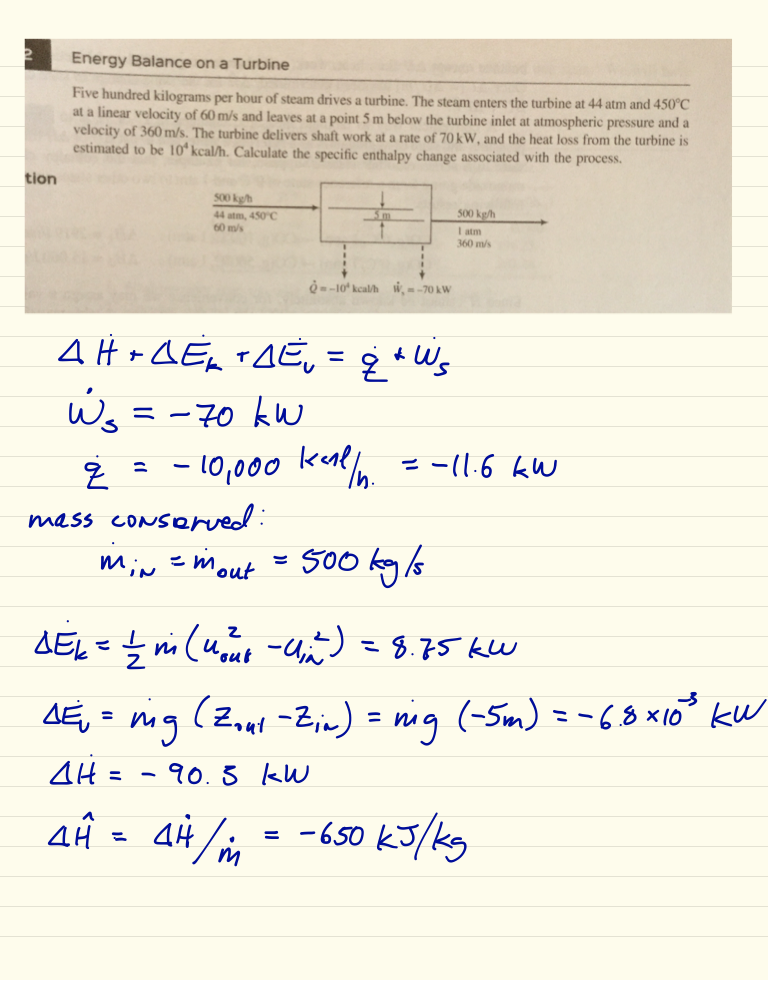
\includegraphics[width=.9\linewidth]{./figs/Turbine1.png}

\subsection{Thermodynamic data}
\label{sec-9-4}
\begin{itemize}
\item Internal energy and enthalpy are \emph{state functions}: they depend only on the intensive properties (\emph{T}, \emph{P}), composition, and state of a material
\item Because they are \emph{energies}, they have no absolute value.  Rather, can only measure/know \emph{changes} in these properties between two states
\item \emph{Measured} by contriving an experiment in which all energy changes other then \(\Delta{U}\) or \(\Delta{H}\) are known.
\item Generally tabulated relative to some (stated or unstated) \emph{reference state}, which is defined to have a value of zero
\item Tabulated in \emph{Perry's}, on line, see Table B.8
\item Or NIST, \url{http://webbook.nist.gov/chemistry/fluid/}

\item Because \ce{H2O} is so important to power generation and other chemical engineering processes, thermodynamic properties of water are tabulated  in \emph{steam tables}
\item Table B.5: saturated steam (on phase equilibrium line), in increments of \emph{T}
\item Table B.6: saturated steam (on phase equilibrium line), in increments of \emph{P}
\item Table B.7: superheated steam (beyond phase equilibrium)
\end{itemize}

\begin{framed}
\noindent \textbf{EXAMPLE} Pressure, specific internal energy, and enthalpy of saturated steam at \SI{133.5}{\celsius}?
\\
\noindent (Table B.6): 3.0 bar, 2543.0 kJ/kg, 2724.7 kJ/kg
\end{framed}


\begin{framed}
\noindent \textbf{EXAMPLE} Specific volume, internal energy, and enthalpy of steam at \SI{400}{\celsius} and 10 bar, relative to triple point.
\\
\noindent At 10 bar, saturation temperature is \SI{179.9}{\celsius} (dew point, Table B.6).  Thus, this must be superheated steam.

(Table B.7): 0.307 m3/kg, 2958 kJ/kg, 3264 kJ/kg
\end{framed}

\begin{itemize}
\item Note that energies are stronger function of \emph{T} than \emph{P}.
\end{itemize}

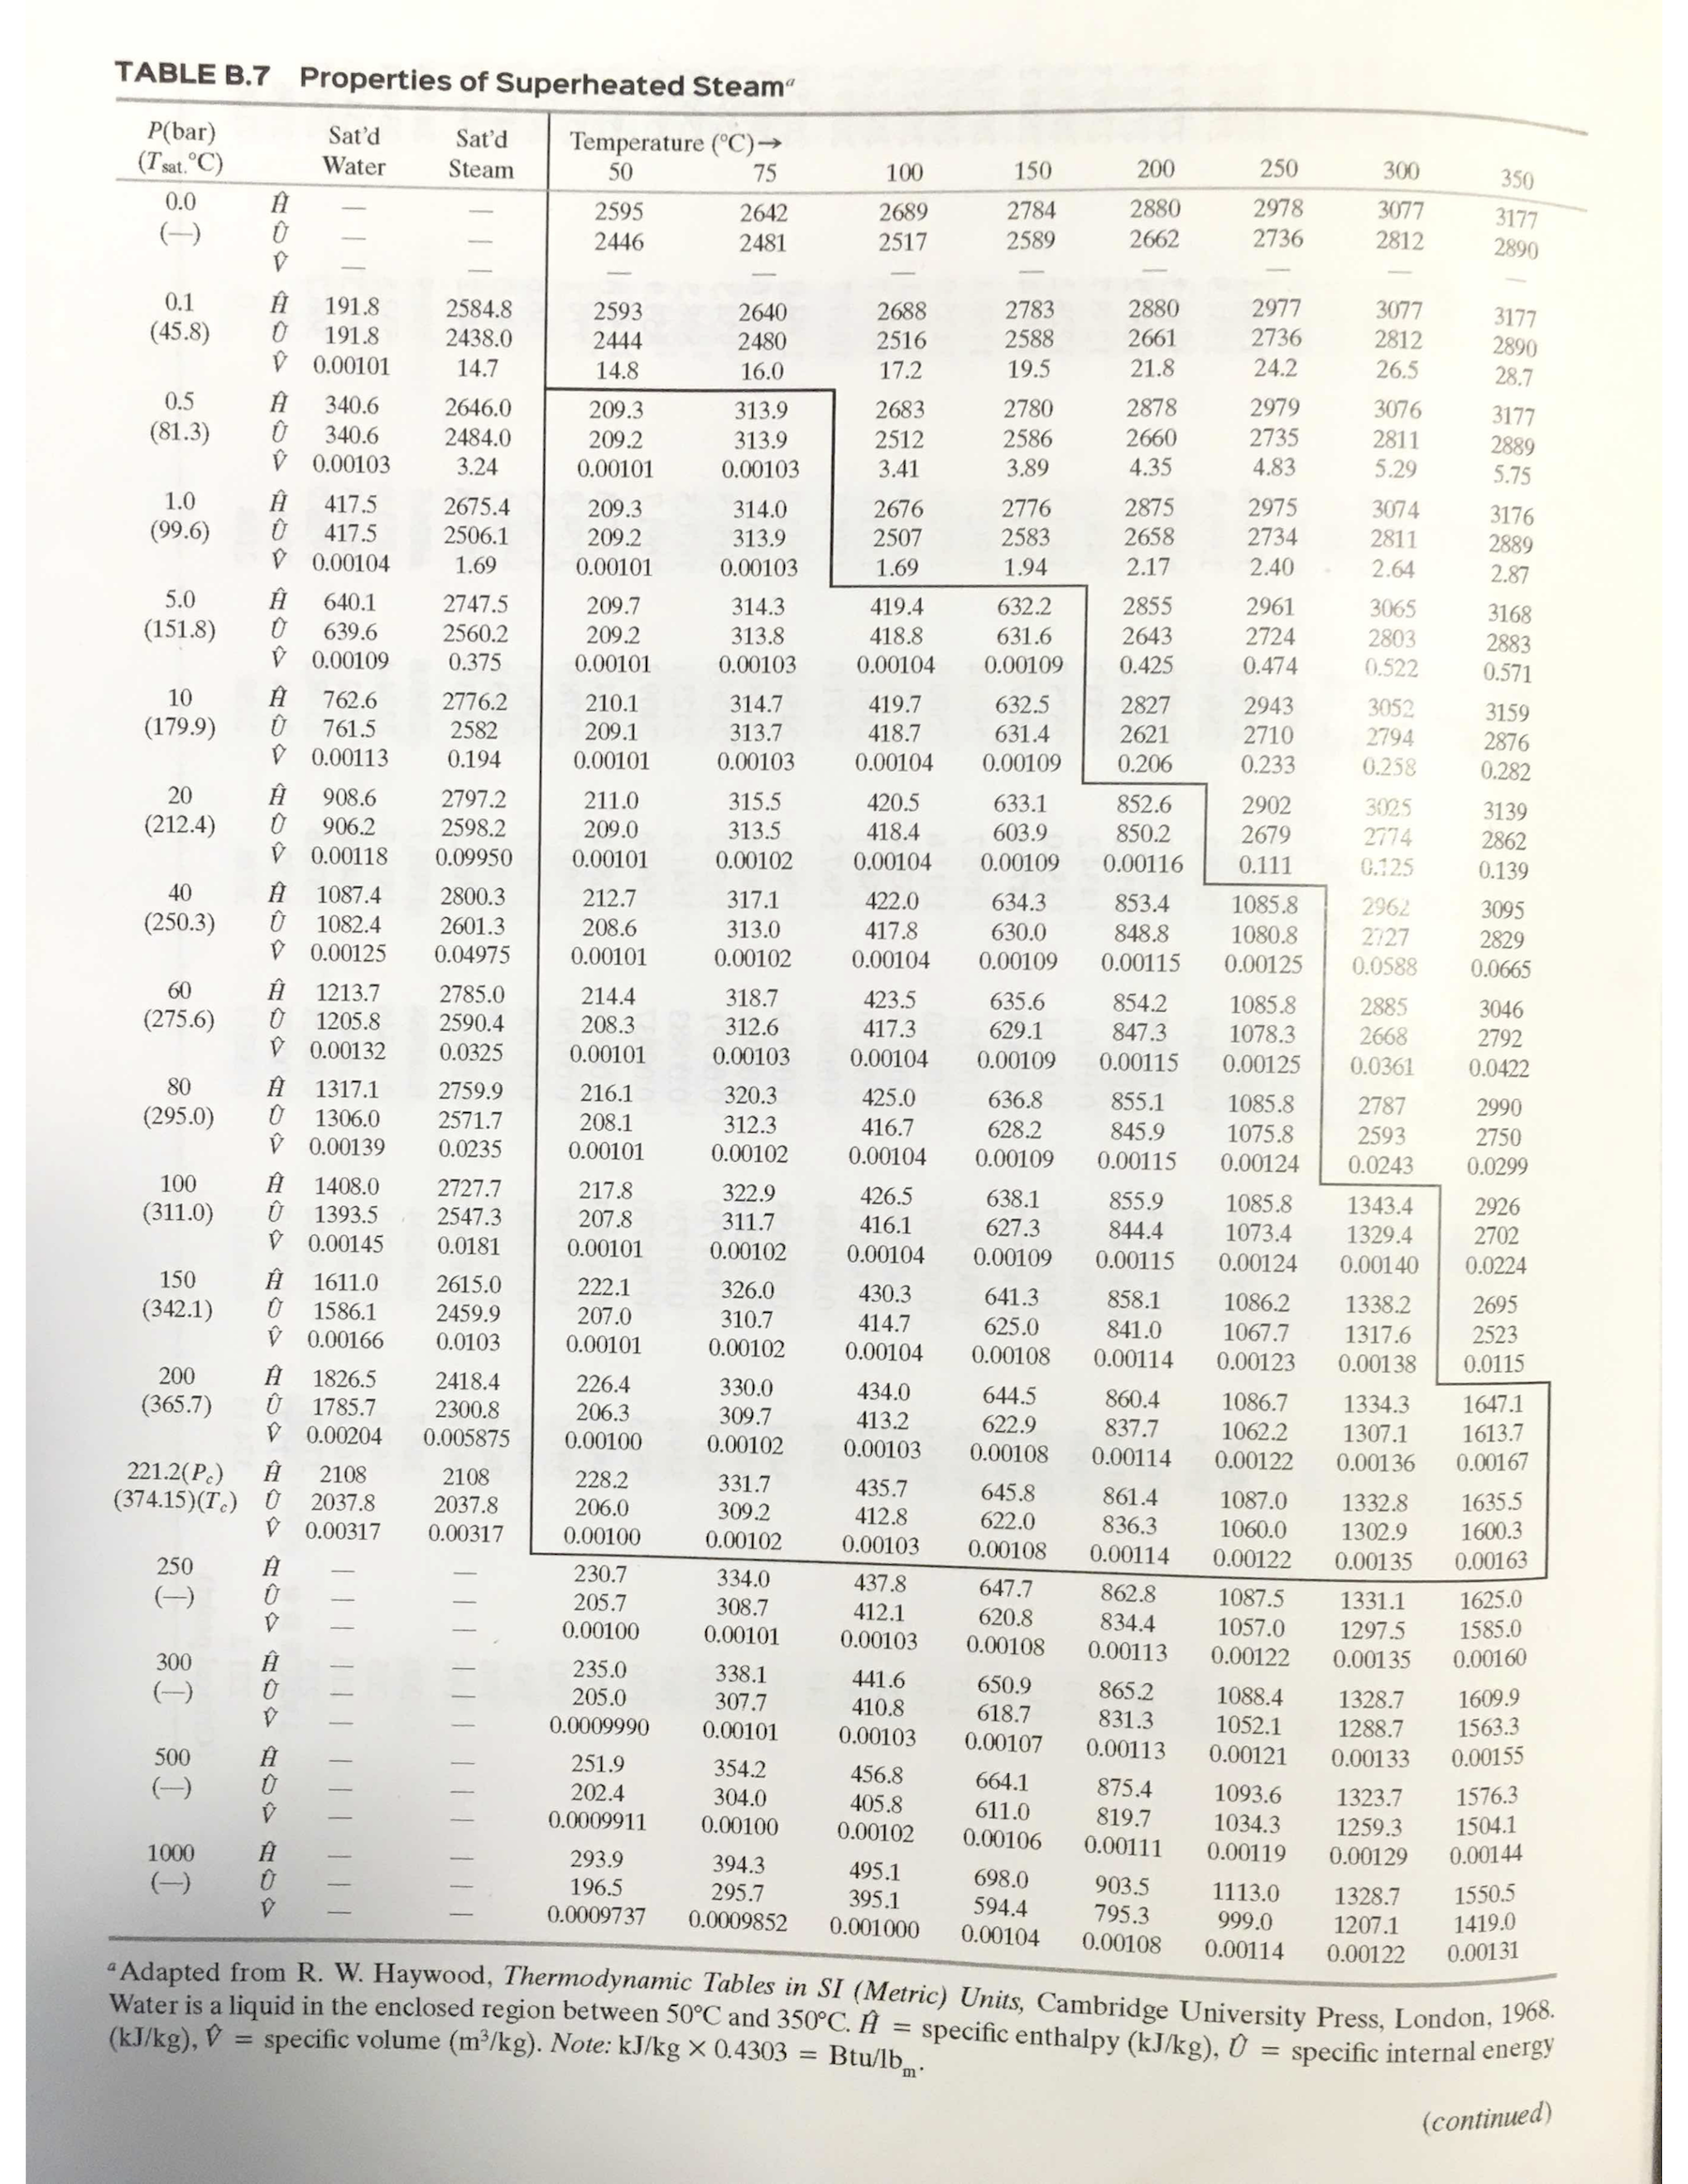
\includegraphics[width=.9\linewidth]{./figs/TableB7.png}

\begin{framed}
\noindent \textbf{EXAMPLE} Steam at 10 bar absolute and \SI{190}{\celsius} superheat enters turbine at \(\dot{m}= 2000\) kg/hr.  Turbine is adiabatic, and effluent is saturated steam at 1 bar.  Work output of turbine?
\\
\noindent Found above that kinetic and potential energy changes are small, so neglect here.

\[ \dot{W}_{s} = \Delta\dot{H} = \dot{m}\Delta\hat{H} \]

\end{framed}

\begin{minted}[frame=lines,fontsize=\scriptsize,linenos]{python}
Pin = 10.  # bar
Tdew = 180. # celsius
Tin = 190. + Tdew

H350= 3159.  # kJ/kg
H400= 3264.  # kJ/kg

Hin = H350 + 20. * (H400 - H350)/(400. - 350.)

print('Interpolated Hin = {0:5.1f} kJ/kg'.format(Hin))

Hout = 2675.
mdot = 2000. # kg/hr

Work = mdot * (Hout - Hin)/3600    # kW

print('Shaft work = {0:5.1f} kW'.format(Work))
\end{minted}

\begin{verbatim}
Interpolated Hin = 3201.0 kJ/kg
Shaft work = -292.2 kW
\end{verbatim}

\subsection{Combined mass and energy balances}
\label{sec-9-5}

\begin{itemize}
\item Example 7.6-1
\end{itemize}
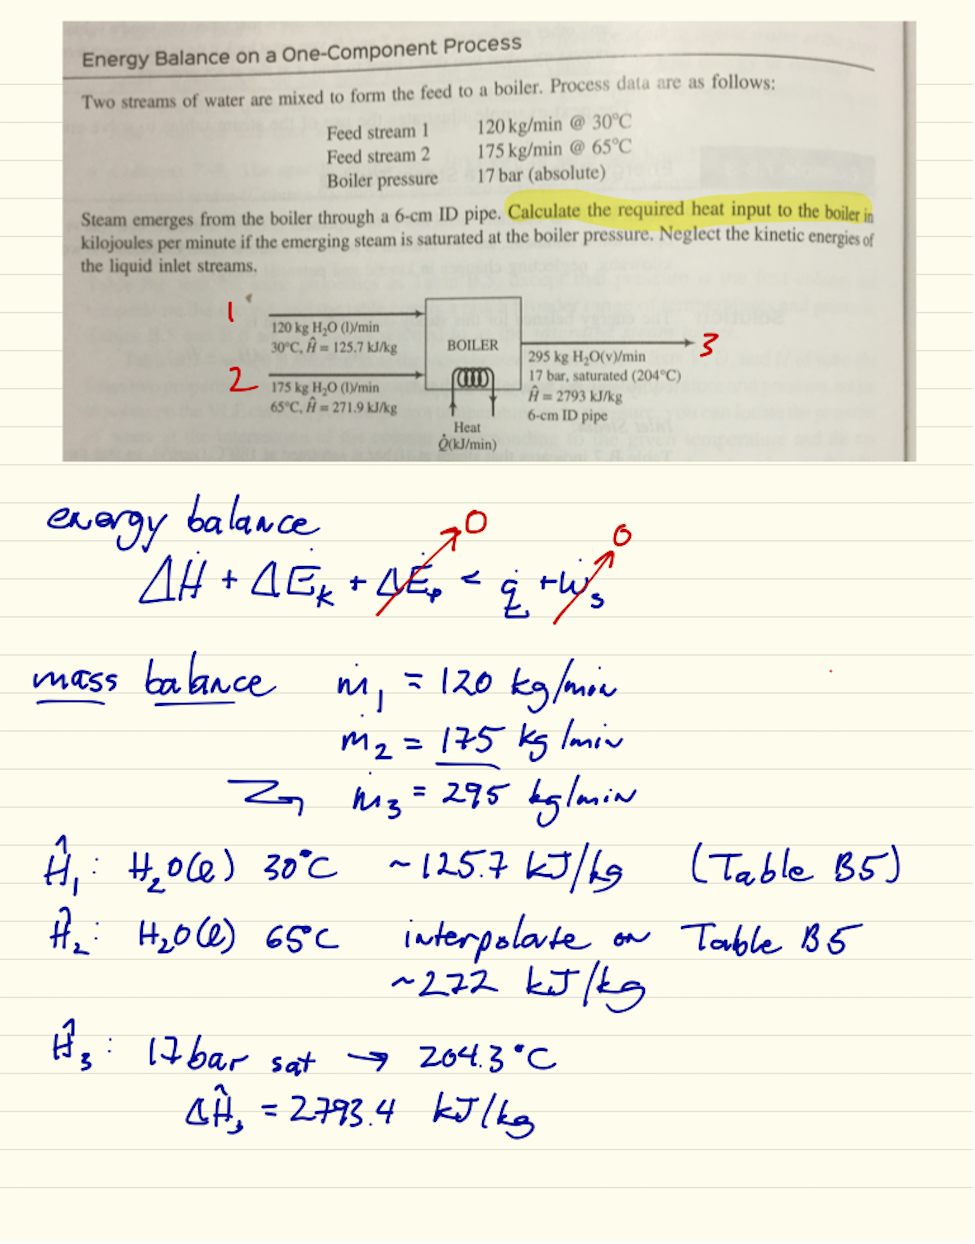
\includegraphics[width=.9\linewidth]{./figs/Example761a.png}

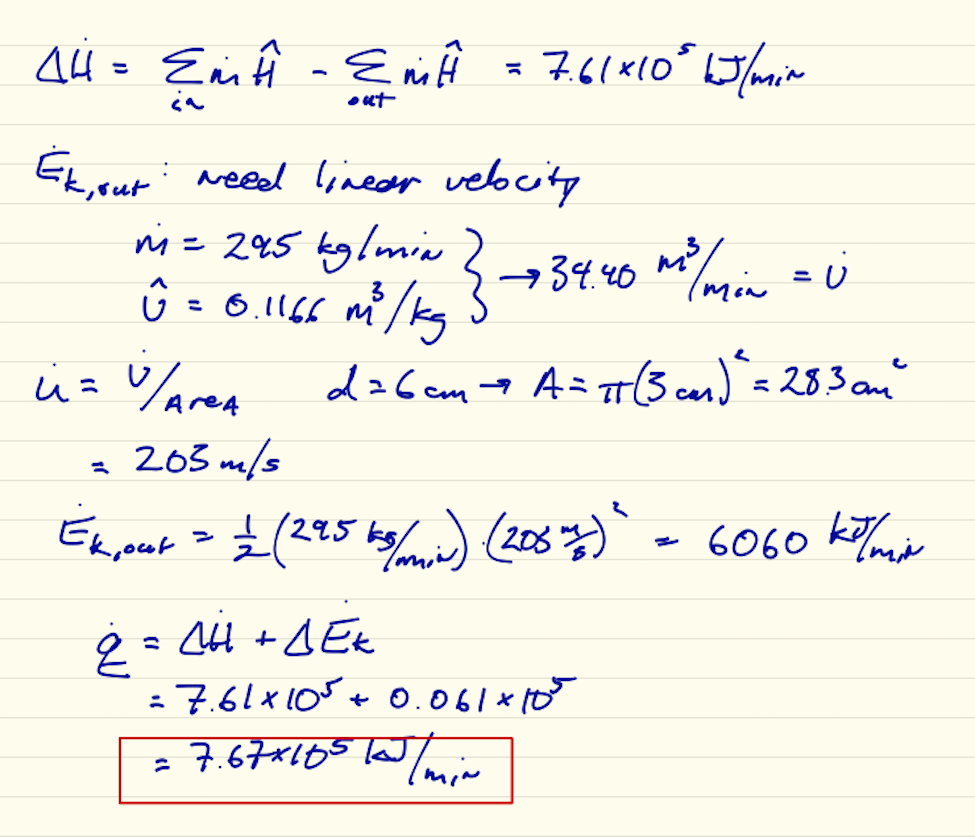
\includegraphics[width=.9\linewidth]{./figs/Example761b.png}

\begin{itemize}
\item Example 7.6-3
\end{itemize}
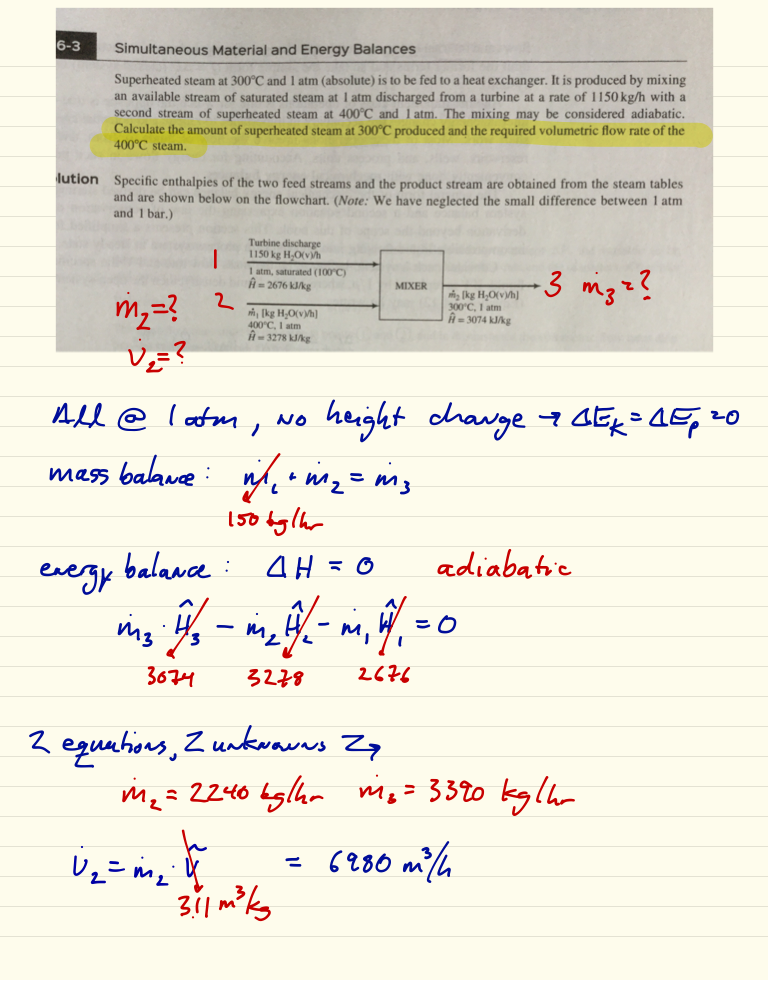
\includegraphics[width=.9\linewidth]{./figs/Example763.png}

\subsection{Mechanical balances}
\label{sec-9-6}
\begin{itemize}
\item Examples to this point emphasize changes involving either change in \emph{T} or chemical composition.  Such processes are often dominated by \(\Delta H\); work, kinetic, and potential terms are generally small
\item Opposite extreme is isothermal, no chemical reaction, e.g. when pumping/moving fluids around

\item General energy balance
\end{itemize}

\[ \Delta\dot{U} + \Delta\dot{E}_{K} + \Delta \dot{E}_{V} - \dot{q} - \dot{W}_{s} -\dot{W}_{f} = 0 \]

\begin{itemize}
\item If we have a single, incompressible fluid (\( \rho = \dot{m}/\dot{V} \) is constant), can simplify energy balance:
\end{itemize}

\[ \frac{1}{2}\dot{m} \Delta u^{2} + \dot{m}g\Delta z + \left( \Delta\dot{U} - \dot{q}\right) - \dot{W}_{s} + \dot{V}\Delta P = 0\]

\begin{itemize}
\item Third term always has a positive friction component:
\end{itemize}

\[ \frac{1}{2}\dot{m} \Delta u^{2} + \dot{m}g\Delta z + \dot{m}\hat{F} - \dot{W}_{s} + \frac{\dot{m}}{\rho}\Delta P = 0\]

\begin{itemize}
\item Neglecting friction and shaft work gives \emph{Bernoulli equation}:
\end{itemize}

\begin{framed}
\[ \frac{1}{2} \Delta u^{2} + g\Delta z  + \frac{1}{\rho}\Delta P = 0\]
\end{framed}

\begin{framed}
\noindent \textbf{Example 7.7-1} Pressure required to push \SI{20}{\liter\per\minute} water 50 m uphill from a 0.5 cm pipe into a 1 cm pipe.
\end{framed}

\includegraphics[width=.9\linewidth]{./figs/Example771.png}

\begin{itemize}
\item Siphon
\end{itemize}

\begin{framed}
\noindent \textbf{Example 7.7-2} Estimate time to siphon 5 gallons out of a gas tank through a 1/4 in i.d. plastic tube.  Assume top tank is large, so its surface doesn't move, and hose end is 2.5 ft below upper fluid level.
\end{framed}

\includegraphics[width=.9\linewidth]{./figs/Example772.png}

\begin{itemize}
\item Water turbine
\end{itemize}

\includegraphics[width=.9\linewidth]{./figs/Example773.png}

\newpage
\section{Energy balances on non-reactive systems}
\label{sec-10}
\subsection{State function}
\label{sec-10-1}
\begin{itemize}
\item Can use any path we want to compute the energy/enthalpy difference between any two well defined points
\item \( A(T_{2},P_{2}) = A(T_{1},P_{1}) + (A(T_{1},P_{2}) -A(T_{1},P_{1})) +  (A(T_{2},P_{2}) -A(T_{1},P_{2})) \)
\begin{itemize}
\item single component, single phase
\item single component, two phase
\item two component, two phase, only one condensible
\item two component, single phase
\item two component, two phase
\end{itemize}
\end{itemize}
\subsection{Isothermal pressure dependence}
\label{sec-10-2}
\begin{itemize}
\item Ideal gas energy/enthalpy \emph{only} a function of \emph{T}
\item Real gas has weak dependence, use tabulation or EOS
\item The volumes of solids and liquids are roughly independent of \emph{P}
\begin{itemize}
\item \(U(T,P_{2}) - U(T,P_{1}) \approx 0\)
\item \(H(T,P_{2}) - H(T,P_{1}) \approx \hat{V}\Delta P\)
\end{itemize}
\end{itemize}

\begin{framed}
\noindent Is it safe to ignore pressure effect in \ce{C2H6} (g, 25C, 1 atm) \ce{-> C2H6} (g, 25C, 30 atm)?  Consider reduced /T/, /P/.
\end{framed}

\begin{minted}[frame=lines,fontsize=\scriptsize,linenos]{python}
Tc = 305.4 # K
Pc = 48.2  # atm

T = 25 + 273 # K
P = 30       # atm

Tr = T/Tc
Pr = P/Pc

print('Tr = {0:5.2f}  Pr = {1:5.2f}'.format(Tr,Pr))
\end{minted}

\begin{verbatim}
Tr =  0.98  Pr =  0.62
\end{verbatim}

\begin{itemize}
\item Generalized compressibility chart
\end{itemize}

\includegraphics[width=.9\linewidth]{./figs/compress.png}

\subsection{Isochoric temperature dependence}
\label{sec-10-3}
\begin{itemize}
\item Energy stronger function of temperature
\item Dependence defined as \emph{heat capacity}, heat flow is \emph{sensible heat}
\item Constant volume heat capacity often tabulated as a polynomial
\end{itemize}

\[ C_{v}(T) = \left ( \frac{\partial\hat{U}}{\partial T} \right )_{v} \]

\[ \hat{U}(T_{2}) - \hat{U}(T_{1}) = \int_{T_{1}}^{T_{2}}C_{v}(T) dT \]

\begin{framed}
\noindent \textbf{Heat capacity example.}  Heat necessary to warm 200 kg \ce{N2O} from 20 to \SI{150}{\celsius} in constant volume vessel?

\[ C_{v} = a + b T, \quad a = 0.855 \text{kJ/kg C}, \quad b = 9.42\times 10^{-4} \text{kJ/kg C}^{2}\]

Integrate!  \(q = \Delta U = 24200\) kJ
\end{framed}

\begin{itemize}
\item Heat flow at constant \emph{pressure} similarly related to enthalpy:
\end{itemize}

\[ C_{p}(T) = \left ( \frac{\partial\hat{H}}{\partial T} \right )_{p} \]

\[ \hat{H}(T_{2}) - \hat{H}(T_{1}) = \int_{T_{1}}^{T_{2}}C_{p}(T) dT \]

\begin{itemize}
\item For liquids and solids, \(C_{p} \approx C_{v}\)
\item For ideal gas, \(C_{p} = C_{v} + R\)
\item For real gas, need an equation, tabulation, or computer program to evaluate
\end{itemize}

\subsection{No data?}
\label{sec-10-4}
\begin{itemize}
\item Correlations, e.g. ``Kopp's rule''
\item For mixtures, assume additive
\end{itemize}

\[ C_{p}(T) \approx \sum_{i} y_{i} C_{p,i}(T) \]

\begin{itemize}
\item Or if dilute, treat as pure
\end{itemize}

\includegraphics[width=.9\linewidth]{./figs/gasheat.png}

\subsection{Phase change}
\label{sec-10-5}
\begin{itemize}
\item phase change involves change in enthalpy at constant \emph{T} and \emph{P}
\item termed ``latent'' heat of transition
\begin{itemize}
\item melting/fusion
\item vaporization/condensation
\end{itemize}
\item tend to be large relative to heat capacity
\item like heat capacity, strong function of \emph{T}, weak function of \emph{P}
\begin{itemize}
\item recall steam tables
\end{itemize}
\end{itemize}

\includegraphics[width=.9\linewidth]{./figs/Latent.png}

\begin{itemize}
\item Recall latent heats can be gotten rigorously from the Clapeyron equation and approximately from Clausius-Clapeyron
\item Trouton's rule an example of a \emph{correlation}.  Note positive correlation between boiling point and enthalpy
\end{itemize}
\[
\Delta H_{v}(\text{kJ/mol}) \approx \left \{ \begin{array}{lcr}
0.088 T_{b} & \text{(K)}& \text{(non-polar liquids)} \\
0.109 T_{b} & \text{(K)}& \text{(water and small alcohols)}
\end{array} \right
\]
\begin{itemize}
\item many other correlations can be found
\item how might you make such a correlation???
\end{itemize}

\subsection{Phase change + mass balance}
\label{sec-10-6}
\includegraphics[width=.9\linewidth]{./figs/MassEnergy1.png}

\begin{minted}[frame=lines,fontsize=\scriptsize,linenos]{python}
import numpy as np
import matplotlib.pyplot as plt
from scipy.optimize import fsolve

def PBs(T):
    A = 6.89272; B= 1203.531; C=219.888 # benzene Antoine, C and mmHg
    logP = A - B/(T+C)
    return 10**logP

def PTs(T):
    A = 6.95805; B= 1346.773; C=219.693 # toluene Antoine, C and mmHg
    logP = A - B/(T+C)
    return 10**logP

T = 50.

xB = 0.4; xT=1-xB

P = xB*PBs(T) + xT*PTs(T)

yB = xB*PBs(T)/P; yT = xT*PTs(T)/P

print('Raoult's Law Pressure = {0:6.1f} mmHg'.format(P))
print('Vapor yB,yT)
\end{minted}

\begin{verbatim}
Pressure =  163.8 mmHg
0.6625107083992408 0.33748929160075913
\end{verbatim}

\includegraphics[width=.9\linewidth]{./figs/MassEnergy2.png}

\subsection{Psychrometric charts}
\label{sec-10-7}
\begin{itemize}
\item Alternative way of representing VLE data
\item Recall phase rule: an air-water vapor mixture has \(2-1+2 = 3\) DOFs, commonly \emph{T}, \emph{P}, \emph{y}
\item Hard to measure \emph{y}, easier to measure ``wet bulb temperature,'' \(T_{wb}\)
\begin{itemize}
\item Temperature of a thermometer with its bulb swathed in wet gauze.  \emph{T} differences measures distance of air from saturation.
\item At dew point, \(T_{wb} = T\)
\item At less than saturation, \(T_{wb} < T\)
\end{itemize}
\item Psychrometric chart summarizes these relationships and other properties of air-water vapor at fixed total \emph{P}
\end{itemize}

\includegraphics[width=.9\linewidth]{./figs/PsychrometricChart.png}

\begin{itemize}
\item Choose \emph{T} and \(T_{wb}\)
\begin{itemize}
\item Find RH
\item Find density
\item Find mixture composition/absolute humidity (all the way to the right)
\item Find dew point (all the way to the left)
\item Find enthalpy of saturated air
\item Find enthalpy at point: follow enthalpy at saturation line; accurate calculations include a small deviation term that we won't worry about
\end{itemize}
\item Paths left and right correspond to cooling and heating air at fixed composition
\end{itemize}

\begin{framed}
\noindent \textbf{Example: air conditioning.} Air at \SI{25}{\celsius}, 80\% RH, and 1 atm is isobarically cooled to \SI{10}{\celsius}.  Calculate the fraction of \ce{H2O} vapor that condenses and the heat removal rate to deliver \SI{1}{\meter\cubed\per\minute} of humid air.
\end{framed}

\includegraphics[width=.9\linewidth]{./figs/AC1.png}

\includegraphics[width=.9\linewidth]{./figs/AC2.png}

\subsection{Non-ideal mixtures}
\label{sec-10-8}
\begin{itemize}
\item Enthalpies additive in ideal mixture
\item Real mixture, \(\hat{H}_{soln} \neq \sum \hat{H}_{i}\)
\item Differential interactions, \ce{H2SO4 + H2O}, or \ce{NaOH + H2O}
\item Can be tabulated as \emph{integral heat of solution}
\begin{itemize}
\item enthalpy to dissolve 1 mole solute in \emph{r} moles solvent (draw picture)
\end{itemize}
\end{itemize}

\begin{table}[htb]
\caption{integral heat of solution of HCl(g) in \ce{H2O} (l)}
\centering
\begin{tabular}{rr}
\hline
\ce{H2O} (mol) & \(\Delta\hat{H}(r)_{soln}\)(298 K)\\
\hline
1 & -26.22\\
10 & -69.49\\
100 & -73.85\\
1000 & -74.68\\
10000 & -74.99\\
100,000 & -75.10\\
$\infty$ & -75.14\\
\hline
\end{tabular}
\end{table}

\begin{itemize}
\item Table reports \(\hat{H}_{soln}\) relative to pure components
\item Alternative reference possible, e.g. \(\hat{H} = \hat{H}(r) - \hat{H}(\infty)\) references infinite dilution
\end{itemize}

\begin{framed}
\noindent \textbf{EXAMPLE solution.}  Adsorb HCl (g) in \ce{H2O} (l).  HCl(g) at \SI{100}{\celsius} and \ce{H2O} at \SI{25}{\celsius} fed to produce \SI{1000}{\kilogram\per\hour} 20.0\%(w/w) HCl at \SI{40}{\celsius}.
\end{framed}

\includegraphics[width=.9\linewidth]{./figs/Mixture1.png}

\includegraphics[width=.9\linewidth]{./figs/Mixture2.png}

\begin{itemize}
\item Enthalpy-concentration chart, normalized to total amount of solution rather than amount of solute

\includegraphics[width=.9\linewidth]{./figs/Formation.png}
\end{itemize}

\includegraphics[width=.9\linewidth]{./figs/TieLine.png}

\subsection{Two-phase, non-ideal mixtures}
\label{sec-10-9}
\begin{itemize}
\item Two two-component phases in equilibrium have \(2-2+2=2\) DOF, e.g. \emph{P} and \emph{T} or some \emph{x}
\begin{itemize}
\item Determines all other properties, e.g. enthalpies
\item Summarized in enthalpy chart like that above, but now lines for liquid and vapor, connected by ``tie lines''
\end{itemize}
\end{itemize}

\includegraphics[width=.9\linewidth]{./figs/EnthalpyComposition.png}

\begin{framed}
\noindent \textbf{EXAMPLE:} Two-phase \ce{H2O}/\ce{NH3} system at 160 F. What are compositions of two phases?  Enthalpies?  Total enthalpy if 95\% of mass is liquid?
\end{framed}

\begin{itemize}
\item Given total composition of system, ``lever rule'' tells us relative fractions of two phases (short segment $\to$ lots of that fraction)
\end{itemize}

\[ \frac{l}{v} = \frac{x_{v} - x_{T}}{x_{T}-x_{l}} \]

\begin{framed}
\noindent \textbf{EXAMPLE: Flash} Aqueous \ce{NH3} stream "flashed" to lower pressure. Very simple unit op to lower \textit{T} and enrich liquid/vapor phases.
\end{framed}

\includegraphics[width=.9\linewidth]{./figs/Flash.png}


\section{Energy balances on reactive systems}
\label{sec-11}
\subsection{Heats of reaction}
\label{sec-11-1}
\begin{itemize}
\item Rearrangements of bonds $\to$ change in enthalpy
\item ``heat of reaction'' defined for specific reaction stoichiometry and (generally) for pure species in specified states
\end{itemize}

\[\ce{CaC2(s) + 2 H2O (l) -> Ca(OH)2 (s) + C2H2 (g)}   \quad \Delta H_{r}(\SI{25}{\celsius},\SI{1}{\atmosphere}) = \SI{-125.4}{\kilo\joule\per\mole}\]

\begin{itemize}
\item Define \emph{endo} and \emph{exothermic}
\item \(\Delta H_{r}\) function of state and conditions
\begin{itemize}
\item Weak function of \emph{P}, strong function of \emph{T} and state
\end{itemize}
\end{itemize}

\[\ce{CH4(g) + 2 O2 (g) -> CO2(g) + 2 H2O (l)} \quad \Delta H_{r} = \SI{-890}{\kilo\joule\per\mole} \]

\[\ce{CH4(g) + 2 O2 (g) -> CO2(g) + 2 H2O (g)} \quad \Delta H_{r} = \SI{-802.3}{\kilo\joule\per\mole} \]

\begin{itemize}
\item \emph{Standard} heat of reaction defined as everything in their most stable states at \SI{25}{\celsius} and 1 atm

\item Enthalpy algebra
\end{itemize}

\[ \sum_{j} \nu_{j}A_{j}=0  \quad \Delta H_{r}(T_{0},P_{0}) \]

\[ n_{j} = n_{j0} + \nu_{j}\xi \]

\begin{itemize}
\item For specific amount of reaction
\end{itemize}

\[ \Delta H = \Delta H_{r} \frac{n_{j}-n_{j0}}{\nu_{j}} = \Delta H_{r} \xi \]

\begin{itemize}
\item Flow context, same idea
\end{itemize}

\[ \dot{n}_{j} = \dot{n}_{j0} + \nu_{j}\xi \]

\[ \Delta \dot{H} = \Delta H_{r} \frac{\dot{n}_{j}-\dot{n}_{j0}}{\nu_{j}} = \Delta H_{r} \xi \]

\begin{framed}
\noindent \textbf{EXAMPLE: Enthalpy of reaction}.  Butane combustion:

\[ \ce{C4H10 (g) + 13/2 O2(g) -> 4 CO2(g) + 5 H2O (l)}\quad \Delta H_{r} =\SI{-2878}{\kilo\joule\per\mole} \]
\end{framed}

\includegraphics[width=.9\linewidth]{./figs/RxnEnthalpy.png}

\begin{itemize}
\item Example of \emph{Hess's Law} - reaction enthalpies are additive
\end{itemize}
\subsection{Formation and combustion reactions}
\label{sec-11-2}
\begin{itemize}
\item In the context of chemical energies, everyone has agreed on a reference state convention
\item Define a ``formation reaction'' to be the (hypothetical) formation of a compound from the constituent elements at \SI{25}{\celsius} and 1 atm
\item Enthalpy of this reaction defined to the  ``heat of formation,'' \(\Delta \hat{H}_{f}\)
\end{itemize}

\[\ce{N2(g) + 2 H2(g) + 3/2 O2 (g) -> NH4NO3 (s)}\quad\Delta \hat{H}^{\circ}_{f}= \SI{-365.14}{\kilo\joule\per\mole}\]

\begin{itemize}
\item By this convention, the enthalpy of formation of the elements is zero
\item Heats of formation measured indirectly, widely tabulated (Table B.1)
\item Easy to show
\end{itemize}

\[ \Delta H^{\circ}_{r} = \sum_{j} \nu_{j} \Delta \hat{H}_{f,j}^{\circ} \]

\begin{itemize}
\item Various methods exist to estimate \(\Delta H_{f}\)
\begin{itemize}
\item bond additivity, quantum mechanics
\end{itemize}

\item Similar concept applies to combustion reaction, defined as enthalpy of complete combustion with all species at standard conditions
\end{itemize}

\[ \ce{C2H5OH (l) + 3 O2(g) -> 2 CO2(g) + 3H2O(l)}\quad \Delta\hat{H}^{\circ}_{c} = \SI{-1366.9}{\kilo\joule\per\mole} \]

\begin{itemize}
\item Similarly tabulated, follows similar additive rule to find enthalpy of any reaction (note sign change):
\end{itemize}

\[ \Delta H^{\circ}_{r} = -\sum_{j} \nu_{j} \Delta \hat{H}_{c,j}^{\circ} \]

\subsection{Energy balances}
\label{sec-11-3}
\begin{itemize}
\item ``Heat of reaction'' method
\begin{itemize}
\item Choose a convenient reference state for each reactant and product, typically ones for with the heat of reaction is known
\item Construct path reactant state $\to$ standard reactants $\to$ standard products $\to$ product state
\item Easy for single reaction
\end{itemize}
\end{itemize}

\[ \Delta \dot{H} = \xi\Delta\hat{H}^{\circ}_{r} + \sum_{out}\dot{n}_{out}\hat{H}_{out}-\sum_{in}\dot{n}_{in}\hat{H}_{in} \]

\begin{itemize}
\item Requires solving for multiple advancements for parallel reactions
\end{itemize}

\[ \Delta \dot{H} = \sum_{i}\xi_{i}\Delta\hat{H}^{\circ}_{r} + \sum_{out}\dot{n}_{out}\hat{H}_{out}-\sum_{in}\dot{n}_{in}\hat{H}_{in} \]

\includegraphics[width=.9\linewidth]{./figs/RxnEnthalpy1.png}

\begin{itemize}
\item ``Heat of formation'' method
\begin{itemize}
\item Choose elements in their standard states as reference
\end{itemize}
\end{itemize}

\[ \Delta \dot{H} = \sum_{out}\dot{n}_{out}\hat{H}_{out}-\sum_{in}\dot{n}_{in}\hat{H}_{in} \]

\includegraphics[width=.9\linewidth]{./figs/RxnEnthalpy2.png}

\begin{itemize}
\item ``Heat of formation'' method nice for multiple reactions
\end{itemize}

\subsection{Adiabatic reactors}
\label{sec-11-4}

\begin{itemize}
\item Sometimes faced with unknown final \emph{T}
\end{itemize}

\includegraphics[width=.9\linewidth]{./figs/Adiabatic.png}

\begin{itemize}
\item Or combined mass and energy
\end{itemize}

\includegraphics[width=.9\linewidth]{./figs/MassEnergy2-1.png}

\subsection{Other applications}
\label{sec-11-5}
\begin{itemize}
\item Heats of solution
\item Combustion
\end{itemize}

\section{Transient processes}
\label{sec-12}
\begin{itemize}
\item General balance around any system or element of a system
\end{itemize}

\begin{framed}
output = input + (generation - consumption) - accumulation
\end{framed}

\begin{itemize}
\item In general can vary with time.  Each term has units amount/time
\end{itemize}

\[ \dot{F}_{out}(t) = \dot{F}_{in}(t) + r_{F}(t) - \frac{dF}{dt} \]

\begin{itemize}
\item For total mass, simplifies because mass cannot be created or destroyed
\end{itemize}

\[ \dot{m}_{out}(t) = \dot{m}_{in}(t) - \frac{dm}{dt} \]

\begin{itemize}
\item Differential equation.  Needs a boundary condition to be solvable.
\end{itemize}

\begin{framed}
\noindent \textbf{Balance on a filling tank}
\end{framed}

\begin{itemize}
\item For chemical reaction, rate related to chemical reaction rate.
\end{itemize}
% Emacs 25.0.50.1 (Org mode 8.2.10)
\end{document}